%
% latex-sample.tex
%
% This LaTeX source file provides a template for a typical research paper.
%

%
% Use the standard article template.
%
\documentclass[12pt]{article}

% The geometry package allows for easy page formatting.
\usepackage{geometry}

% Load up special logo commands.
\usepackage{doc}

% Package for formatting URLs.
\usepackage{hyperref}

% Packages and definitions for graphics files.
\usepackage{graphicx}
\usepackage{epstopdf}
\usepackage{setspace}
\usepackage{framed}
% To generate dummy text
\usepackage{lipsum}
\usepackage{mwe}

% To adjust title location
\usepackage{titling}

\usepackage{amsmath}
\usepackage{amssymb}
\usepackage[utf8]{inputenc}
\usepackage{url}
\usepackage{listings}
\usepackage{caption}
\usepackage{subcaption}
\usepackage{booktabs}
\usepackage[T1]{fontenc}
\usepackage[ruled]{algorithm2e}
\usepackage{csvsimple}

%\doublespacing
\onehalfspacing
%\setlength{\droptitle}{5em}   % This is your set screw

\makeatletter    
\def\@maketitle{
	\centering
	
%	{\Huge \bfseries \sffamily \@title }\\[4ex] 
	{\LARGE \@title }\\ [60mm]
	
\includegraphics[width = 40mm]{boun} \\[5mm]
	{\large \@author}\\[5mm] 
	\@date\\

}
\makeatother

% set up graphics path
\graphicspath{{./img/}}

\newcommand{\myitem}{\refstepcounter{enumi}\item[$*$\theenumi.]}

%\DeclareGraphicsRule{.tif}{png}{.png}{`convert #1 `dirname #1`/`basename #1 .tif`.png}

%
% Set the title, author, and date.
%

%\tit1{Cmpe 492  Final Project \\[10mm] Midterm Report }
%\tit2{A Matchmaking \& Ranking System\\ via \\ Bayesian Inference}
\title{Cmpe 492  Final Project \\[1mm] Final Report \\[60mm] Player Rating Estimation\\ via \\[3mm] Bayesian Inference}
	 

\author{Mustafa Onur Eken\\ advised by A. Taylan Cemgil}
\date{2016}

%
% The document proper.
%

\geometry{
	a4paper,
	total={170mm,257mm},
	left=30mm,
	top=25mm,
	right=30mm,
	bottom=30mm,
}
\begin{document}
% Add the title section.
\maketitle
\thispagestyle{empty}
\newpage
% Add an abstract.
%\abstract{}

% Add various lists on new pages.
\pagebreak
\tableofcontents

\pagebreak




%\listoffigures
%\pagebreak
%\listoftables
% Start the paper on a new page.
%\pagebreak

%
% Body text.
%
\section{Introduction \& Motivation}

Player rating systems are essential nearly to any game in situated in different contexts (video games, sports etc). This need arises from the fact that an \textit{unbalanced} match is not enjoyable to any of it's competitors. In an \textit{unbalanced}  match, there is a high variation among the skills of the competitors, therefore a remarkable challenge is not achieved and inadequate amount of fun is generated.

Assuming the fact that the skill levels of the players in a match is the dominant factor affecting the result of that match, if we could figure out skill levels of players of a particular game then we could arrange \textit{balanced} matches that are entertaining for both highly and poorly skilled players. In additions to this, estimating skills of players with respected to a particular model enables us to predict results of future matches. Intuitively a more complex model would possess less of bias and would yield more accurate predictions.

 All in all, rating systems attempt to measure goodness of players, for instance, in most national football leagues, wins worth 3 points, draws worth 1 point and losses worth 0 point. At the end of the season, we obtain an estimate of skills/goodness of competing teams in that league according to this underlying model. Some can argue that it ignores many details therefore it is too simple and inaccurate. Another disadvantage of this model is that it does not specify rules to compute probabilities for possible outcomes of a future match. 
 
 To attack this problem, many context-free rating systems are proposed but Elo, Glicko, TrueSkill are the most prominent ones \cite{minka2006trueskill}. In this project we assume a particular model (resembling to the one proposed by TrueSkill algorithm) governing winning/losing probabilities in reality. Afterwards, we attempt to estimate skills of players by training on their past data, i.e. match results. Our model necessitates that we perform Bayesian inference to figure out skills of players, therefore we implemented three different methods to achieve inference in this project. We run the algorithms both on synthetic and real data and interpret the results.
 
In the next section, we tell briefly about the significant works in this field as well as the state of the art methods. After that, in section 3, we explain the model we assumed in depth and overview different practices to perform Bayesian inference. We explain the algorithms (MCMC, Expectation Propagation ) we have used in this project in detail in the following subsections. In section 4, we visualize the results we have obtained with various tables and plots and interpret them in section 5. We conclude by discussing how this project can be extended in section 6 and we include the full source code in the last section.

%In this project we are going to study and implement a generalized and improved version of Elo rating system, developed by Microsoft Research , \textit{TrueSkill}. It is generalized because matches are not constrained as to be one versus one and unlike Elo, \textit{TrueSkill }learns more from the stalemates. In addition, it converges on players' ratings faster.


\section{State of the Art}

\subsection{Elo}
Arpad Elo constructed a rating system for the board game Chess in 1959. According to his modeling \cite{elo1978chess}, rating of a player is a unit-less positive number. The probabilities for different outcomes of a match is a function of skills, $s_i$, of competing players. Players exhibit a \textit{performance} according to their skills. Performance $p_i \sim \mathcal{N}(p_i;s_i,\beta^2)$, in a sense, is a noisy version of a player's skill. The probability that player 1 wins is calculated as follows, where $\phi$ is the cumulative density function of zero-mean, unit-variance Gaussian:
$$P(p_1 > p_2 | s_1, s_2) = \phi (\frac{s_1 - s_2}{\sqrt{2} \beta}) $$
When the actual game outcome of the game is observed skills are updated so that their sum remains the same. Let the actual outcome $y = 1$ if player 1 wins, $y=-1$ if player 2 wins and $y=0$ if it's a stalemate. Elo update is calculated as follows: $s_1 \leftarrow s_1 + \delta y$ and $s_1 \leftarrow s_2 + \delta y$
$$\delta = \alpha \beta \sqrt{\pi} \left( \frac{y+1}{2} - \phi \left(\frac{s_1 - s_2}{\sqrt{2} \beta}\right) \right)$$
Here $\alpha$ is between 0 and 1 and represents the significance of new observations compared to past. This rating system is still in use on many platforms although it has a few drawbacks.
\begin{itemize}
	\setlength\itemsep{-1mm}
	\item Competitions has to be one player versus one player. \textit{Elo} does not cover the case when multiple players compete in a game and the outcome is a permutation of the players to signify ranks.
	\item A new player's skill is provisional until he plays a decent number of matches.
\end{itemize}

\subsection{Glicko \& TrueSkill}
\textit{Glicko} \cite{glickman1999parameter} and \textit{TrueSkill} \cite{minka2006trueskilll} attempts to tackle these problems and generalize underlying idea proposed in \textit{Elo} rating system. \textit{Glicko} suggests modeling of a player's skill as a belief distribution (in particular a Gaussian distribution) rather than representing it with a single number. \textit{TrueSkill} extends this idea to adapt it to matches with multiple teams and players.

Let $k$ teams compete in a match. Team assignments $A_j$ are non-overlapping, in other words, $A_j \cap A_i = \emptyset$ if $i \neq j$. The outcome $r = (r_1, ... , r_k) \in \{1, ..., k\}$. Probability of the outcome is modeled as a function of skills of players and team assignments $P(r | s, A)$. Through Bayes' rule we get the following posterior distribution for skills of players.
$$p(s | r, A) = \frac{P(r|s,A) p(s)}{P(r | A)}$$
Skill is represented as a random variable $s_i \sim \mathcal{N}(s_i;\mu_i,\sigma^2_i)$ where $\mu_i$ is the point estimate of it and $\sigma_i$ is the uncertainty associated with it. Similarly, as in the \textit{Elo} rating system, it is assumed that players generate a performance based on their skills $p_i \sim \mathcal{N}(p_i;s_i,\beta^2)$. Furthermore, teams performances are computed by $t_j = \sum_{i \in A_j} p_i$. This model can be represented with a factor graph compactly. See Figure \ref{factor_graph} for an example factor graph representation.

\begin{figure}[!ht]
	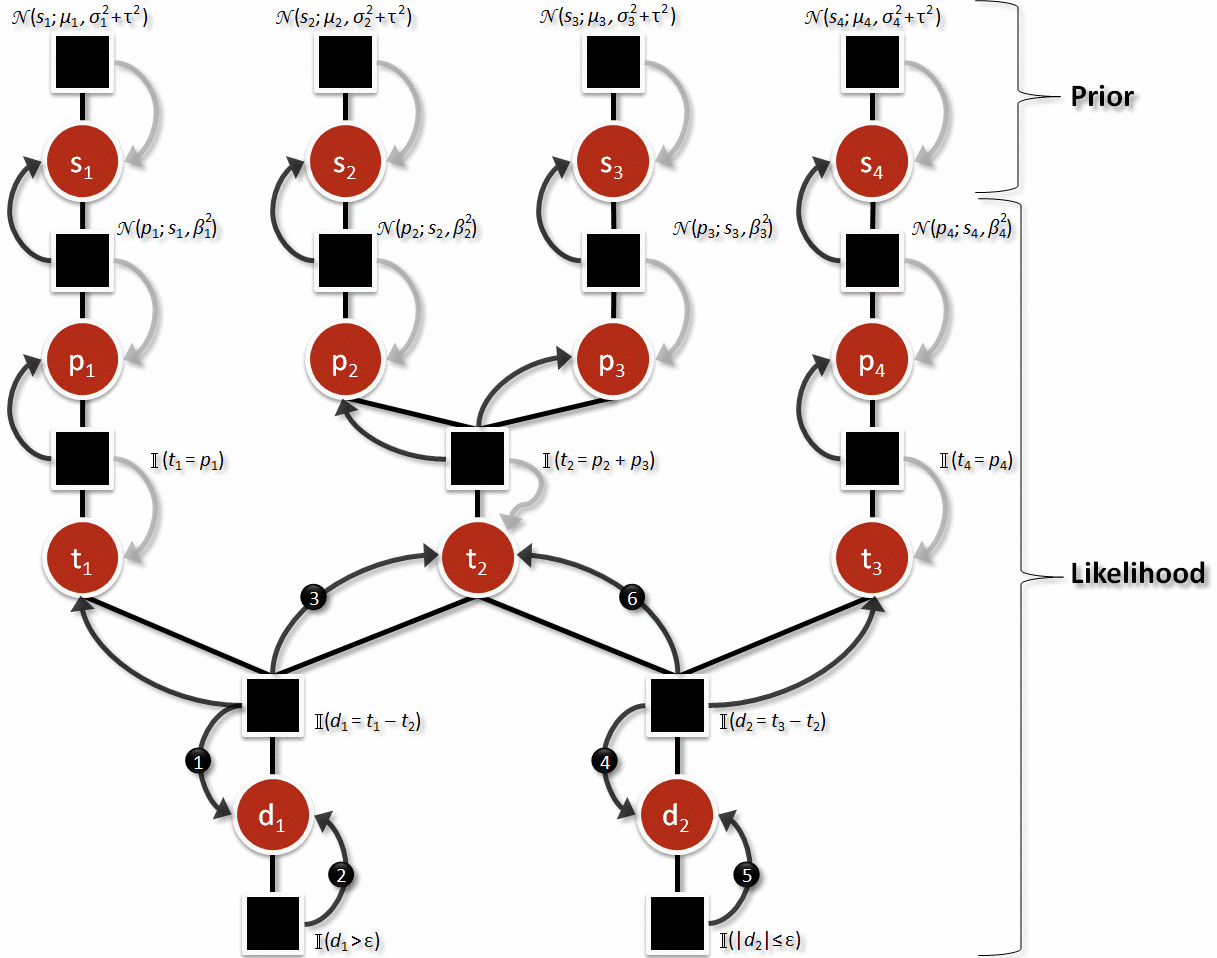
\includegraphics[width=1\columnwidth]{factor_graph}
	\caption{Factor graph representation of \textit{TrueSkill} model for a particular match where $k = 3$, $A_1 = \{1\}$, $A_2 = \{2,3\}$, $A_3 = \{4\}$, $r = (1,2,2)$ i.e. team 1 won, team 2 and 3 draw.}
	\label{factor_graph}
\end{figure}

The see Figure \ref{comp_fact_1} and \ref{comp_fact_2} for interpretation of (comparison/result) factors on the bottom of the graph.


\begin{figure}[!ht]
	\begin{subfigure}{0.45\columnwidth}
		\centering
		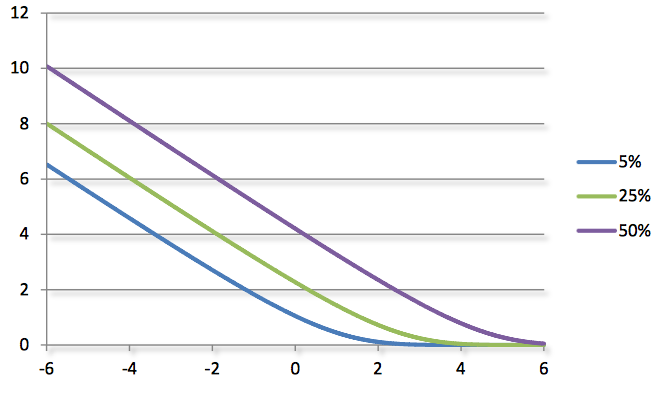
\includegraphics[width=1\columnwidth]{11}
		\caption{$\mathbb{I}( \cdot > \epsilon)$ \textit{i.e. win}. Notice this indicates a major update in means if an upsetting result is observed.}		
	\end{subfigure}%
	\hfill
	\begin{subfigure}{.45\columnwidth}
		\centering
		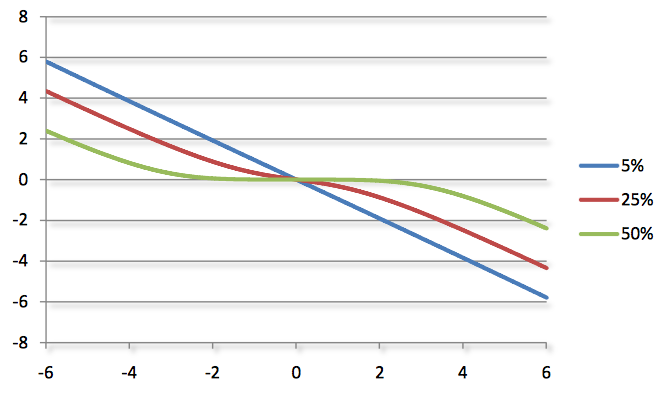
\includegraphics[width=1\columnwidth]{12}
		\caption{$\mathbb{I}( \cdot \leq |\epsilon|)$ \textit{i.e. draw}. Notice this indicates a major update in means only when difference is far from zero.}
	\end{subfigure}
	
	\caption{Function $V$ \textit{i.e. mean update}. x-axis represents the skill difference between winning team and losing team.}
	\label{comp_fact_1}
\end{figure}

\begin{figure}[!ht]
	\begin{subfigure}{.45\columnwidth}
		\centering
		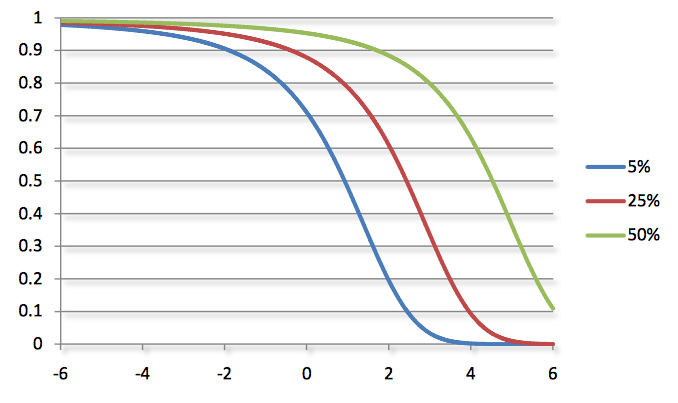
\includegraphics[width=1\columnwidth]{21}
		\caption{$\mathbb{I}( \cdot > \epsilon)$ \textit{i.e. win}. Notice this indicates a major reduction in uncertainties if an upsetting result is observed.}
	\end{subfigure}%
	\hfill
	\begin{subfigure}{.45\columnwidth}
		\centering
		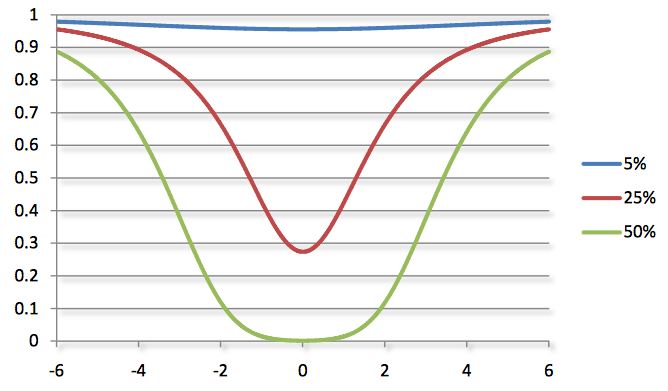
\includegraphics[width=1\columnwidth]{22}
		\caption{$\mathbb{I}( \cdot \leq |\epsilon|)$ \textit{i.e. draw}. Notice this indicates a major update in uncertainties only when difference is far from zero}
	\end{subfigure}	
	\caption{Function $W$ \textit{i.e. uncertainty update}. x-axis represents the skill difference between winning team and losing team.}
	\label{comp_fact_2}
\end{figure}

In principle \textit{TrueSkill} assumes this model and uses \textit{Expectation Propagation} algorithm to infer skill distributions. EP is a deterministic approximation algorithm that can be considered a generalization of a well-known exact inference algorithm used in factor graphs known as \textit{Belief Propagation}/\textit{Sum-Product algorithm} \cite{loeliger2001factor}.

\section{Methods}
In this project we aim to demonstrate Bayesian skill inference (as done in \textit{TrueSkill}) via three different methods both on synthetic data that we generate and on real-world data such as Tennis, football, basketball match results from 2015-2016 season. First two algorithms, namely Metropolis-Hastings and Gibbs sampler, are two different instances of a method known as Markov Chain Monte Carlo sampling. Here, we perform inference by stochastic approximation. In the third method we implement \textit{TrueSkill}'s EP algorithm \cite{minka2001ep} to perform deterministic approximate inference according to the model described above.

\subsection{Model}
Models exist to capture and explain the real world dynamics of various incidents. For instance, Newton's equations is a model to explain the physical motions of the objects situated in the space. Similarly laws of thermodynamics define a model to capture relation between heat, temperature and energy, work. Models can be accurate or inaccurate with respect to some criteria and this depends on the complexity of the model. 

In this project for our Markov Chain Monte Carlo (MCMC from now on) algorithms we propose a particular model. When it comes to Expectation Propagation (EP from now on) algorithm we assume \textit{TrueSkill}'s model. Following are the rules of our model.
\begin{itemize}
	\singlespacing
	\item Let a game $G$ is played by $n$ different players, i.e. $p_i$, $i \in \{1,2,\dots,n\}$ where each $p_i$ denotes a player. 
	\item A match of the game $G$ takes place between a number of teams $k \in \{2,3,\dots\}$
	\item In a match, each team $t_j$, $j \in \{1,2,\dots,k\}$ is a set of players with size $n_j \in \{1,2,\dots\}$
	\item In a match, intersection of any two different team is an empty set.
	\item Each player $p_i$ has a fixed unit-less skill value $s_i \in (0,50)$ associated with itself.
	\item The skill value of a team $w_i$ is the sum of skill values of it's members, i.e. $w_i = \sum_{p_j \in t_i} s_j$
	\item Matches with more than 2 competitors/teams are collapsed down to it's components that are atomic matches between any two team competed in the match. See Tables \ref{collapse_1} and \ref{collapse_2}
	\begin{table}[!ht]
		\centering
		\begin{tabular}{@{}cc@{}}
			\toprule
			\textbf{Name} & \textbf{Rank} \\ \midrule
			Team A & 1 \\
			Team B & 2 \\
			Team C & 3 \\ \bottomrule
		\end{tabular}\hspace{5mm}
		\begin{tabular}{@{}cc@{}}
			\toprule
			\textbf{Name} & \textbf{W/L/D} \\ \midrule
			Team A & W \\
			Team B & L \\ \bottomrule
		\end{tabular} 
		\begin{tabular}{@{}cc@{}}
			\toprule
			\textbf{Name} & \textbf{W/L/D} \\ \midrule
			Team A & W \\
			Team C & L \\ \bottomrule
		\end{tabular}
		\begin{tabular}{@{}cc@{}}
			\toprule
			\textbf{Name} & \textbf{W/L/D} \\ \midrule
			Team B & W \\
			Team C & L \\ \bottomrule
		\end{tabular}
		\caption{An example how matches with more than 2 competitors/teams is collapsed down to it's components.}
		\label{collapse_1}
	\end{table}

	\begin{table}[!ht]
		\centering
		\begin{tabular}{@{}cc@{}}
			\toprule
			\textbf{Name} & \textbf{Rank} \\ \midrule
			Team A & 1 \\
			Team B & 2 \\
			Team C & 2 \\ \bottomrule
		\end{tabular}\hspace{5mm}
		\begin{tabular}{@{}cc@{}}
			\toprule
			\textbf{Name} & \textbf{W/L/D} \\ \midrule
			Team A & W \\
			Team B & L \\ \bottomrule
		\end{tabular} 
		\begin{tabular}{@{}cc@{}}
			\toprule
			\textbf{Name} & \textbf{W/L/D} \\ \midrule
			Team A & W \\
			Team C & L \\ \bottomrule
		\end{tabular}
		\begin{tabular}{@{}cc@{}}
			\toprule
			\textbf{Name} & \textbf{W/L/D} \\ \midrule
			Team B & D \\
			Team C & D \\ \bottomrule
		\end{tabular}
		\caption{An example how matches with more than 2 competitors/teams is collapsed down to it's components.}
		\label{collapse_2}
	\end{table}
	
	\item Outcome, $r$, of atomic matches is a function of skills $w_i$, $w_j$ of two teams $t_i$ and $t_j$.
	\item In an atomic match teams are named as team 1 and team 2.
	\item Outcome $r \in \{1,-1,0\}$ where $1$ indicates win of team 1, $-1$ indicates win of team 2 and $0$ indicates a draw.
	\begin{figure}
		$$
			p(r | w_1, w_2) = 
			\begin{cases} 
			\exp{(|w_1-w_2|, c_1, c_2)} & \text{if } r = 0 \\
			(1 - \exp{(|w_1-w_2|, c_1, c_2)}) * \sigma(w_1 - w_2, c_3)       & \text{if } r = 1 \\
			(1 - \exp{(|w_1-w_2|, c_1, c_2)}) * \sigma(w_2 - w_1, c_3)       & \text{if } r = -1
			\end{cases}
		$$
		\caption{Definition of the win/lose/draw model}
		\label{model1}
	\end{figure}


	\item Decay parameter of exponential function is set $c_2 = 0.05$
	\item Steepness parameter of sigmoid function is set $c_3 = 0.06$ 
	\item Draw factor parameter is set $c_1 = 0.33$, is the y-intercept of exponential function. It regulates draw probabilities together with decay parameter. For example, when skills of teams are equal to each other this model estimates the chance of draw as 33\%. If draws are more likely in a particular type of game it can be set set higher. See Figures \ref{bi_exp}, \ref{sigmo}, \ref{sigmo_2}
	\item We assume that initially all skills $s_i \sim \mathcal{U}(s_i;0,50)$
	\item We can represent the model we described using a Bayesian network. See an example in Figure \ref{baynet_1} and \ref{baynet_2}
	\item We get the joint probability distribution $P(s_1, s_2, \dots, s_n, w_1, w_2, \dots, w_k, r_1, r_2, \dots)$
	
	
	\begin{figure}[!ht]
		\centering
		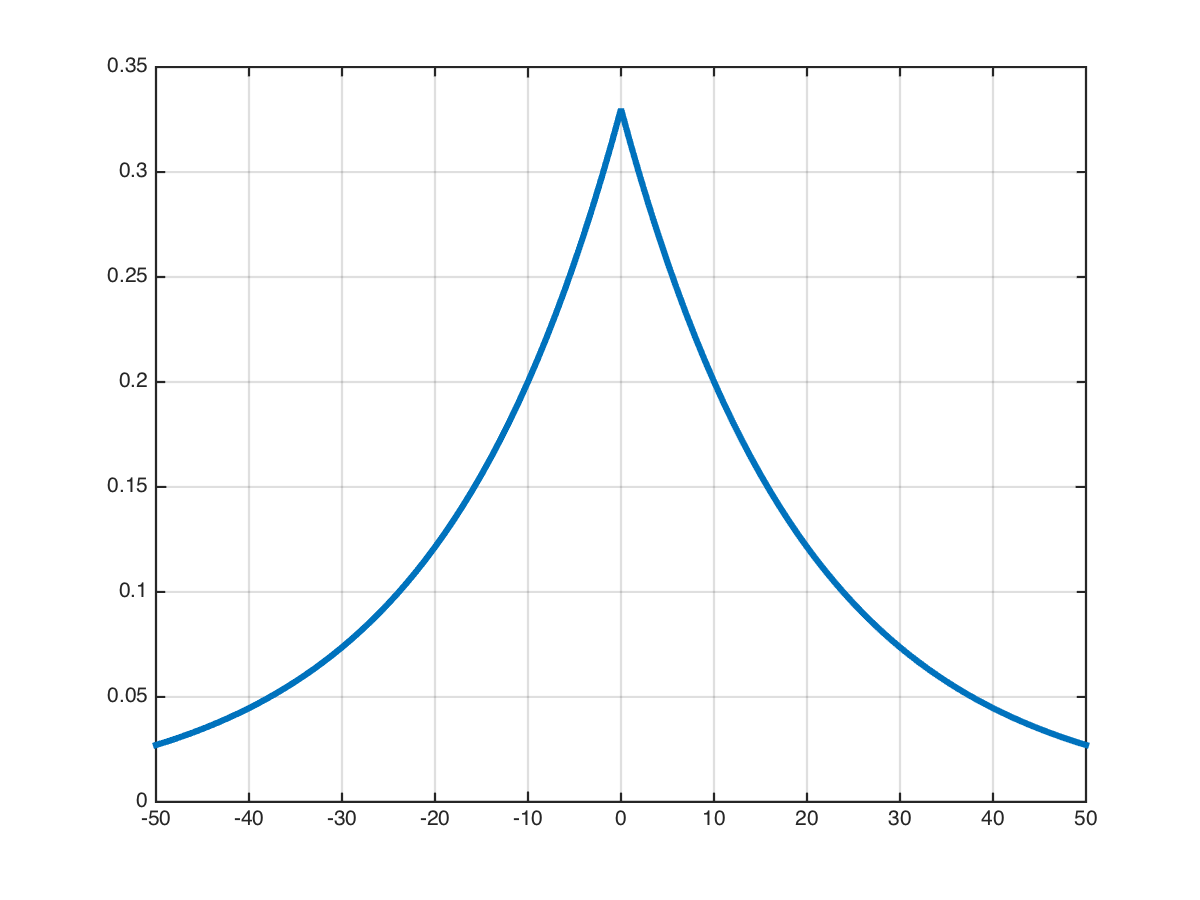
\includegraphics[width=0.7\columnwidth]{bi_expo}
		\caption{$p(r = 0 | w_1, w_2)$ with parameters, $c_1 = 0.33$, $c_2 = 0.05$}
		\label{bi_exp}
	\end{figure}
	
	\begin{figure}[!ht]
		\centering
		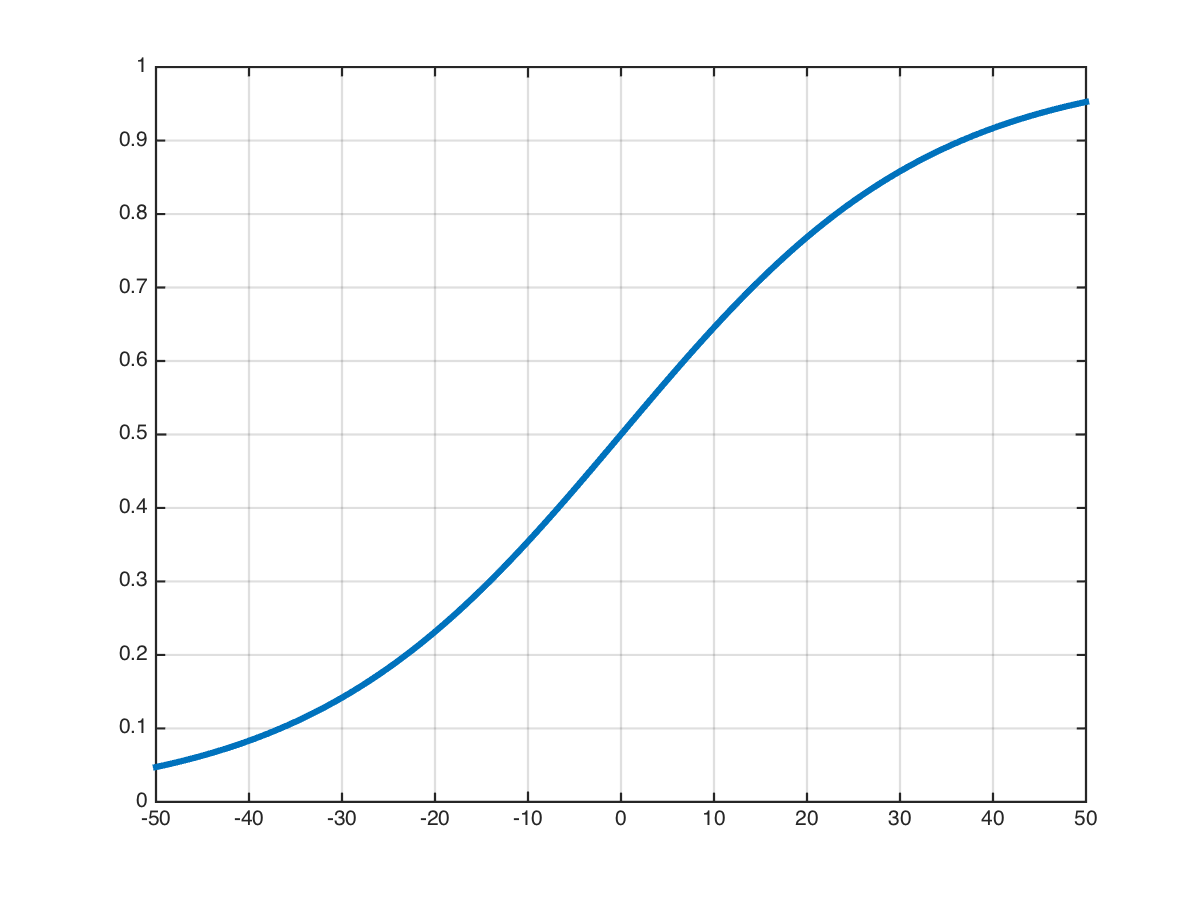
\includegraphics[width=0.9\columnwidth]{sigmo}
		\caption{$\sigma(x, c_3) = \frac{1}{1+ \exp(-c_3 x)}$ with parameter, $c_3 = 0.06$. Also when $c_1 = 0$, $p(r = 1 | w_1, w_2)$ collapses down to sigmoid}
		\label{sigmo}
	\end{figure}

	\begin{figure}[!ht]
		\centering
		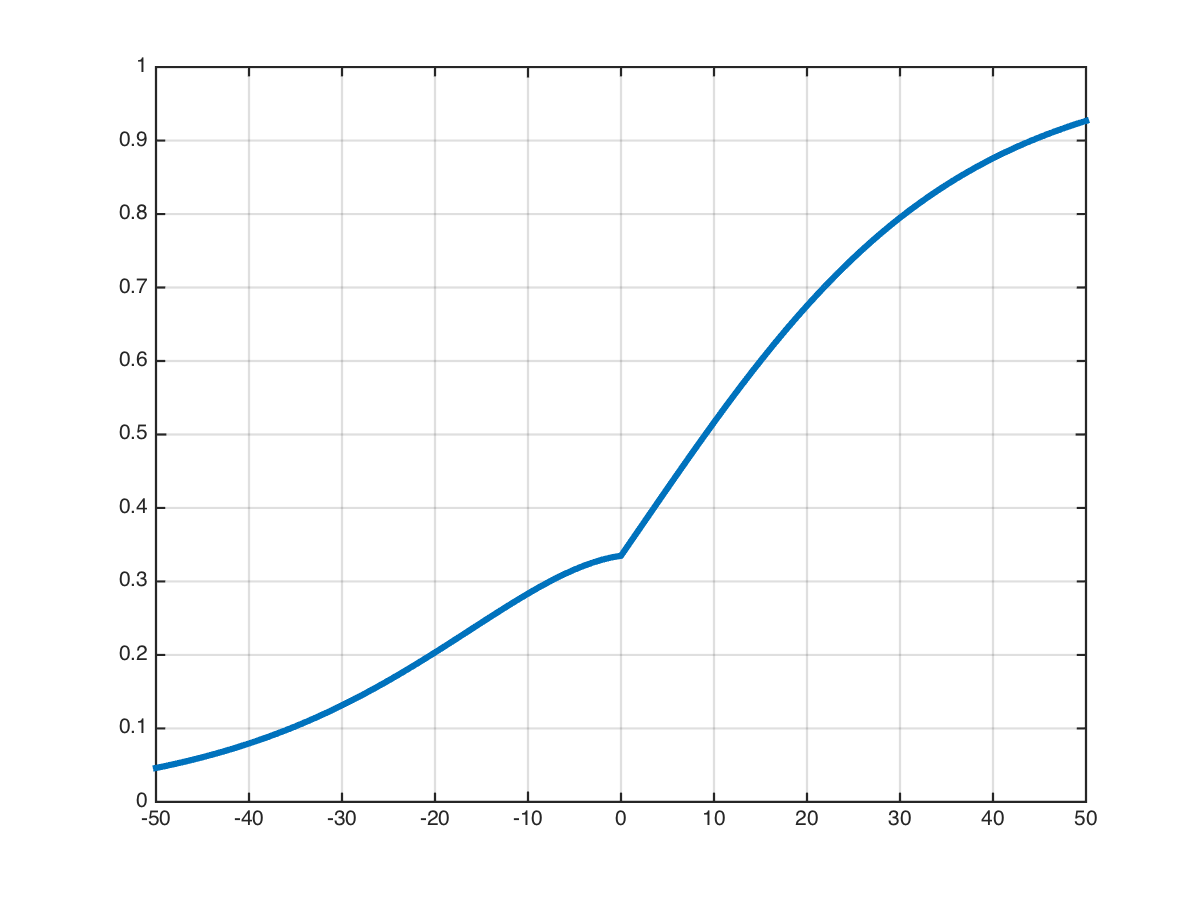
\includegraphics[width=0.9\columnwidth]{sigmo_2}
		\caption{$p(r = 1 | w_1, w_2)$ with parameters, $c_1 = 0.33$, $c_2 = 0.05$, $c_3 = 0.06$.}
		\label{sigmo_2}
	\end{figure}
	
	
	
	\begin{figure}[!ht]
		\centering
		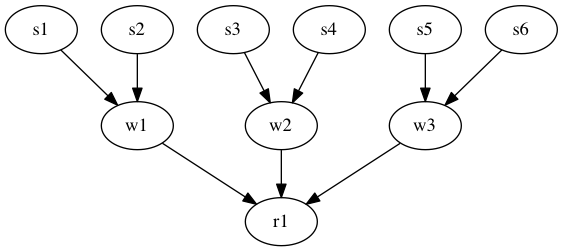
\includegraphics[width=0.7\columnwidth]{baynet_1}
		\caption{An example visual representation of a match with 3 teams each having 2 members. Notice that this match contains more than 2 competitors. See Figure \ref{baynet_2} for decomposed version.}
		\label{baynet_1}
	\end{figure}
	
	\begin{figure}[!ht]
		\centering
		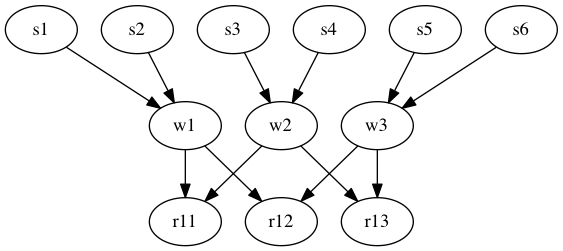
\includegraphics[width=0.7\columnwidth]{baynet_2}
		\caption{Decomposed version of the Bayesian network shown in Figure \ref{baynet_1}. Note that we perform decomposition in order to allow simple probability distribution functions for outcomes, i.e. }
		\label{baynet_2}
	\end{figure}

	\begin{figure}[!ht]
		\centering
		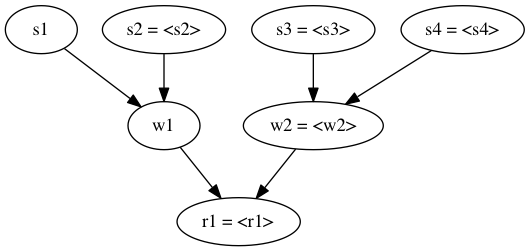
\includegraphics[width=0.7\columnwidth]{baynet_3}
		\caption{Example network with instanciated variables.}
		\label{baynet_3}
	\end{figure}
\end{itemize}
\clearpage


\subsection{Inference}
%Recall that out joint probability distribution is $p(s_1, s_2, \dots, s_n, w_1, w_2, \dots, w_k, r_1, r_2, \dots)$. 
To estimate the skill distributions we are going to construct a Bayesian network whose terminal/result nodes are observed (i.e. fixed) and attempt to figure out the posterior distribution of skills of players. \textit{Variational Bayesian methods }(approximate), \textit{Monte Carlo methods }(approximate), \textit{Belief Propagation algorithm }(exact), \textit{Assumed Density Filtering }(approximate) and \textit{Expectation Propagation }(approximate) are some significant methods for inference \cite{minka2001family}.

Exact methods in continuous domain are often impractical due to integrals intractable to calculate. For that reason approximate algorithms are preferred. Especially Metropolis-Hastings algorithm to sample from a given target distribution via forming an implicit Markov chain is very general. We implement this method in this project. Another MCMC method that we implement is Gibbs sampler because we can analytically come up with conditional distribution of individual skills and can sample from it comfortably which is a must for Gibbs sampler.

Furthermore we implemented Expectation Propagation algorithm as described in \cite{minka2006trueskilll}, therefore model assumed for this algorithm is different than we described in Section 3.1 and it is slightly more complex. You can find a brief description of \textit{TrueSkill}'s model in Section 2.2.

\subsubsection{Markov Chain Monte Carlo}
Recall our joint probability distribution.
$$p(s | w, r=Data) = p(s_1, s_2, \dots, s_n | w_1, w_2, \dots, w_k, r_1=\hat{r_1}, r_2=\hat{r_2}, \dots)$$
$$p(s | w, r=Data) = \frac{p(w,r=Data | s)p(s)}{p(w, r=Data)}$$
$$p(s | w, r=Data) = \frac{p(w,r=Data | s)p(s)}{\int p(w, r=Data | s) p(s) ds}$$
Since $s \sim \mathcal{U}(0,50)$, $p(s)$ does not vary. It is a constant. In addition, the relation ship between $w$ and $s$ is deterministic. Given $s$, one can calculate $w$  with confidence of 100\%. Therefore this expression simplifies down to:
$$p(s | r=Data) = \frac{p(r=Data | s)}{\int p(r=Data | s) ds}$$
$$p(s | r=Data) \propto p(r=Data | s)$$

\newpage

\paragraph{Metropolis-Hastings Algorithm}
The task in MH algorithm is fairly simple, see Figure \ref*{mh} for description of the algorithm. It is insensitive if the target distribution is normalized or not which is a nice feature. We used a multivariate Gaussian distribution as out proposal. The mean of the Gaussian is the last point reached in the space and variance is given as input by the supervisor depending on the sensitivity of the target distribution. We observed in our tests that when the dimensionality of the data grows (i.e. more players and matches) small perturbations in the input/variable result in enormous changes in the output/probability. This is a behaviour we would not favor because it increases the rejection rate. On the other side, one must be careful when choosing a less aggressive proposal because it can lead to inadequate exploration of the space.

When computing output/probability for a given configuration/point in the space, we may have to deal with really small numbers if the size of the dataset is large. To prevent errors originate from the representation of floating numbers in computers we transform some computations to logarithmic scale.

\begin{figure}[!ht]
	\centering
	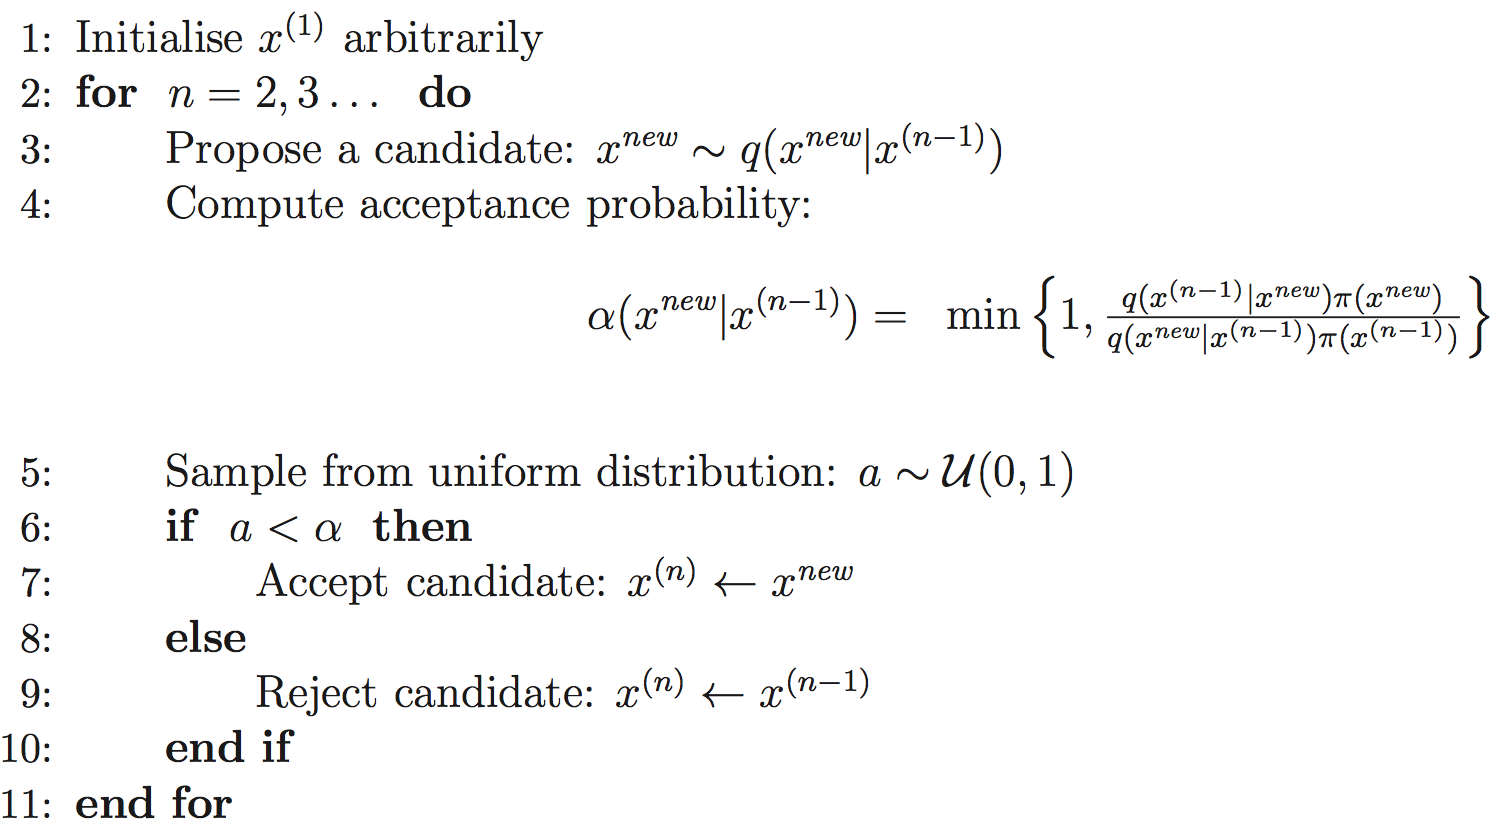
\includegraphics[width=1\columnwidth]{mh}
	\caption{Metropolis-Hastings algorithm.}
	\label{mh}
\end{figure}

\paragraph{Gibbs Sampler}

We can go further and calculate conditional probabilities for individual skill variables. Consider the atomic match visualized in Bayes network in Figure \ref{baynet_3}
$$p(s_1 | \hat{s_2}, \hat{s_3}, \hat{s_4}, \hat{r_1}) = \frac{p(\hat{r_1} , s_1, \hat{s_2}, \hat{s_3}, \hat{s_4})}{\int_{s_1} p(\hat{r_1} , s_1, \hat{s_2}, \hat{s_3}, \hat{s_4})}$$

Where $\hat{v}$ denotes the instantiation of that variable. It is represented in the example network as v = <v>. The denominator is only a normalizing constant. In fact $p(\hat{r_1} , s_1, \hat{s_2}, \hat{s_3}, \hat{s_4}) = p(\hat{r_1} | s_1, \hat{s_2}, \hat{s_3}, \hat{s_4}) * p(s_1) * p(\hat{s_2}) * p(\hat{s_3}) * p(\hat{s_4})$ and since prior distributions of skills are a constant as well we can plug them in the normalizing constant $Z$. We get the following conditional distribution:

$$p(s_1 | \hat{s_2}, \hat{s_3}, \hat{s_4}, \hat{r_1}) = \frac{p(\hat{r_1} | s_1, \hat{s_2}, \hat{s_3}, \hat{s_4})}{Z}$$

We had defined this expression in the first place! (see Section 3.1, Figure \ref{model1}). This indicates that we indeed can use Gibbs sampler once we can draw samples from the distribution given in Figure \ref{model1}. Here we choose a numerical way for solving this problem. We compute the unnormalized cumulative distribution numerically by calculating the distribution function at various points and computing a running sum to obtain data points. These data points mimic cumulative distribution function Then we apply multinomial resampling on obtained data points, see Figure \ref*{multinom}. We transform these computations to logarithmic scale to prevent numerical truncation errors. When size of the dataset and number of the players involved grows we have to deal with really small probabilities. 



\begin{figure}[!ht]
	\centering
	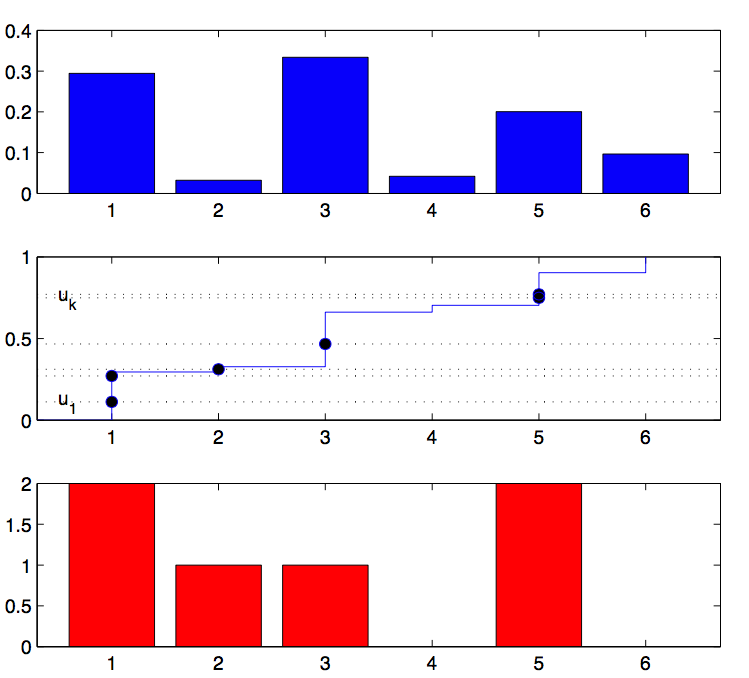
\includegraphics[width=0.55\columnwidth]{multinom}	
	\caption{Multinomial resampling. Taken from \cite{cemgil2009notes}}
	\label{multinom}
\end{figure}

\begin{figure}[!ht]
	\centering
	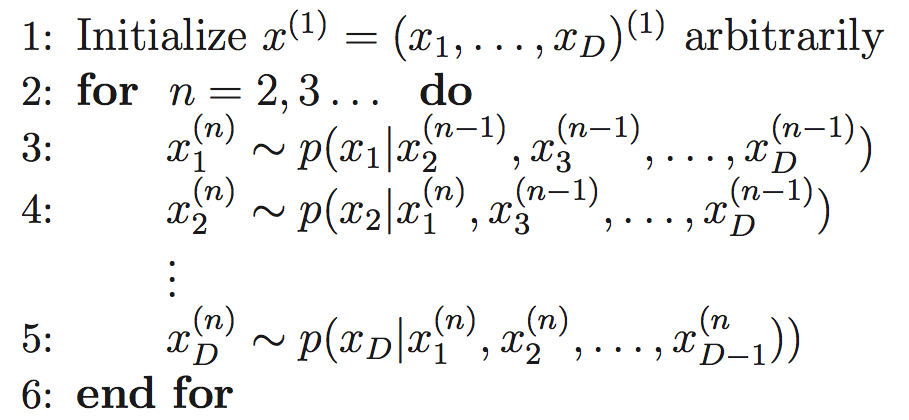
\includegraphics[width=0.55\columnwidth]{gibbs}	
	\caption{Gibbs sampler}
	\label{gibbs}
\end{figure}


\subsubsection{Expectation Propagation}
\paragraph{Factor Graphs and Belief Propagation}
Factor graphs are bipartite graphs over variables and local factors. Local factor together form the global function over all variables when multiplied with each other. Therefore, factor graphs formalize the independence of local factors, Figure \ref{fg}. Factor graphs are more general than Bayes networks therefore a Bayes network can be re-written as a factor graph when factors are defined as conditional probability distributions. The sum-product algorithm \cite{loeliger2001factor} (a.k.a. belief propagation) defines a procedure to marginalize product of factors (in Bayesian case, it corresponds to marginalization of joint probability distribution). Very roughly, it involves multiplication of factors and integrating out of variables which is intractable most of the time. Therefore in principle it works but in reality it is highly impractical.
\begin{figure}[!ht]
	\centering
	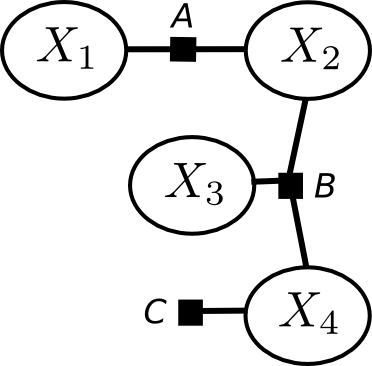
\includegraphics[width=0.2\columnwidth]{fg}	
	\caption{An example factor graph. $G(x_1, x_2, x_3, x_4) = A(x_1, x_2) B(x_2, x_3, x_4) C(x_4)$}
	\label{fg}
\end{figure}

EP follows this general approach: Given a factor graph whose marginal (we are interested in) is hard to compute, approximate it by a simpler graph whose marginal is easy to compute. We replace each factor $f_\alpha$ by an approximate factor $\tilde{f_\alpha}$. Often we choose approximating distribution/factor to be from the exponential family. 

A decent procedure to approximate while keeping the error on the marginal distribution minimum is as follows: Start with an empty factor graph. For each factor $f_\alpha$, incorporate it into the current approximating distribution $q$ by multiplication. This yields some new distribution $q^i$ that is not in the approximating family (exponential family), so project it into the set of all approximating distributions using KL divergence. This is known as \textit{Assumed density filtering}. A problem with this approach is that the order used to traverse factors affect how good the approximation of marginal will be.

Expectation propagation fixes this problem by looping through factors many times. Each of the time, old approximation of a factor $f_\alpha$ is removed from the global approximation $q^{i-1}$ instead exact factor is plugged in back by multiplying. Then, the obtained global distribution (that is not in the family we would like it to be in) is projected to the approximating family using KL divergence.
\clearpage
\begin{algorithm}[H]
	\textit{Initialize}. Set $q^0$ to uniform
	\ForEach{factor $f_\alpha$}{
		\For{i=m...j+1}{
			1. \textit{Refinement} Incorporate exact factor into the approximation \\
				\Indp $q^{+\alpha} \propto q^{i-1} f_\alpha$ \\
			\Indm 2. \textit{Projection} Compute the new approximate distribution by projecting into approximating family \\
				\Indp $qî = \arg \min_q \mbox{KL}(q^{+\alpha} \| q)$ \\
		}
	}
	\caption{Assumed Density Filtering}
	\label{adf}
\end{algorithm} \vspace{5mm}

\begin{algorithm}[H]
	\textit{Initialize}. Set $q^0$ to uniform \\
	\Repeat{until convergence}{
		1. Choose a factor $f_\alpha$ to refine \\
		2. \textit{Refinement}. Remove the previous approximation from global approximation. Incorporate the exact factor \\
		\Indp $q^{\setminus \alpha} \propto \frac{q^{i-1}}{f_\alpha}$ \\
		$q^{+\alpha} \propto f_\alpha q^{\setminus \alpha}$ \\
		\Indm 3. \textit{Projection}. Compute the new global approximate distribution by projecting into approximating family \\
		\Indp $qî = \arg \min_q \mbox{KL}(q^{+\alpha} \| q)$
	}
	\caption{Expectation Propagation}
	\label{ep}
\end{algorithm}


\section{Results}
\paragraph{Synthetic Data}
We first, generated synthetic data in order to test the algorithms in various configurations. Generated synthetic players are assigned a \textit{"reel skill"} value. Teams are formed randomly. The match results are generated according to the model we assumed in Figure \ref{model1}. One important thing here to notice is that, we have shown reel skills on the plots concerned with EP algorithm as well as concerned with MCMC algorithms. But recall that EP is not expected to guess the reel skills assigned because the underlying model with EP algorithm is different than we specified for MCMC algorithms to work on. In other words, skill findings of EP algorithm has its own scaling. But this does not mean that EP is expected to guess match results from test data (which is generated according to our custom model, See Figure \ref{model1}) incorrectly, on the contrary, all algorithms are expected to perform well when tested, See Section 7.
\paragraph{Real-World Data}
Afterwards, we tested three algorithms on real-world data, namely, tennis data (match results in Grand Slam tournaments of 2012-2013), football data (match results in German, Spanish, Turkish, English primary national leagues), basketball data (match results of Nba 2015-2016 regular season). We fetched all datasets and preprocessed them so that they have the form shown in Table \ref{data_form}.

\begin{table}[!ht]
	\centering
	
	\begin{tabular}{@{}ccc@{}}
		\toprule
		\textbf{Team 1} & \textbf{Team 2} & \textbf{Result} \\ \midrule
		Munich          & Dortmund        & 1               \\
		Karlsruhe       & Köln            & 0               \\
		Stuttgart       & Hamburg         & -1              \\
		...             & ...             & ...             \\ \bottomrule
	\end{tabular}
	\caption{Form of the ready data (csv)}
	\label{data_form}
\end{table}

\section{Conclusion \& Discussion}
When test results are examined we see that MCMC methods are computationally more expensive than EP algorithm, overall they take more time to complete the specified number of iterations. When the number of training data size is small, we, as expected, observe high uncertainties in the estimated distributions of skills, which is undesirable because it leads to inaccurate predictions. 

For all algorithms we do not observe a very high prediction accuracy but when looked careful one can see that the success criterion of this approach is another measure. We predict a result which has the maximum likelihood among all results but we are confident about our prediction only by the percentage of the likelihood of predicted result. For instance if we estimate probabilities for possible outcomes for a match as (W:0.5, L: 0.3, D:0.2) and we would pick 'W' as our prediction. But this means that if this particular match takes place infinitely many times then we expect player 1 to win on 50\% of those matches. Keeping this in mind, a good measure of for quality of our prediction system would be the quantitative similarity between \textit{percentage of correct guesses} and \textit{mean of confidences for guesses}.

Lastly, MCMC algorithms are expected to find \textit{shifted} reel skills in some particular cases. For instance, if actual/reel skills of players are very close to each other and located nearly on the middle ($\sim$ 25) of the rating interval (0,50) then even though a large dataset and large number of iterations are used in executing algorithm, exact estimation of reel skills cannot be expected because the solution would not be unique. I.e. a new set of reel skills shifted from the original values by a constant term would \textbf{also} yield the current training set we have.

\section{Future Work}
One aspect of this project to extend is the following idea: Instead of taking match results as \{1,-1,0\} we can take exact match results such as 98-88 (in the case of basketball) and consider the differences between scores. The first problem emerging here is that a hand-crafted model would be undesirable because it would only work for given game domain. For instance, a match result of 5-1 in football indicates a dominating win whereas a match result of 107-102 in basketball does not indicate a dominating win. It would be interesting to design an algorithm which would adjust/adapt a model to capture the scale/dynamics of the game under focus.

% Generate the bibliography.
\bibliography{refs}
\bibliographystyle{unsrt}


\clearpage
\section{Tests}
\begin{figure}[!ht]
	\centering
	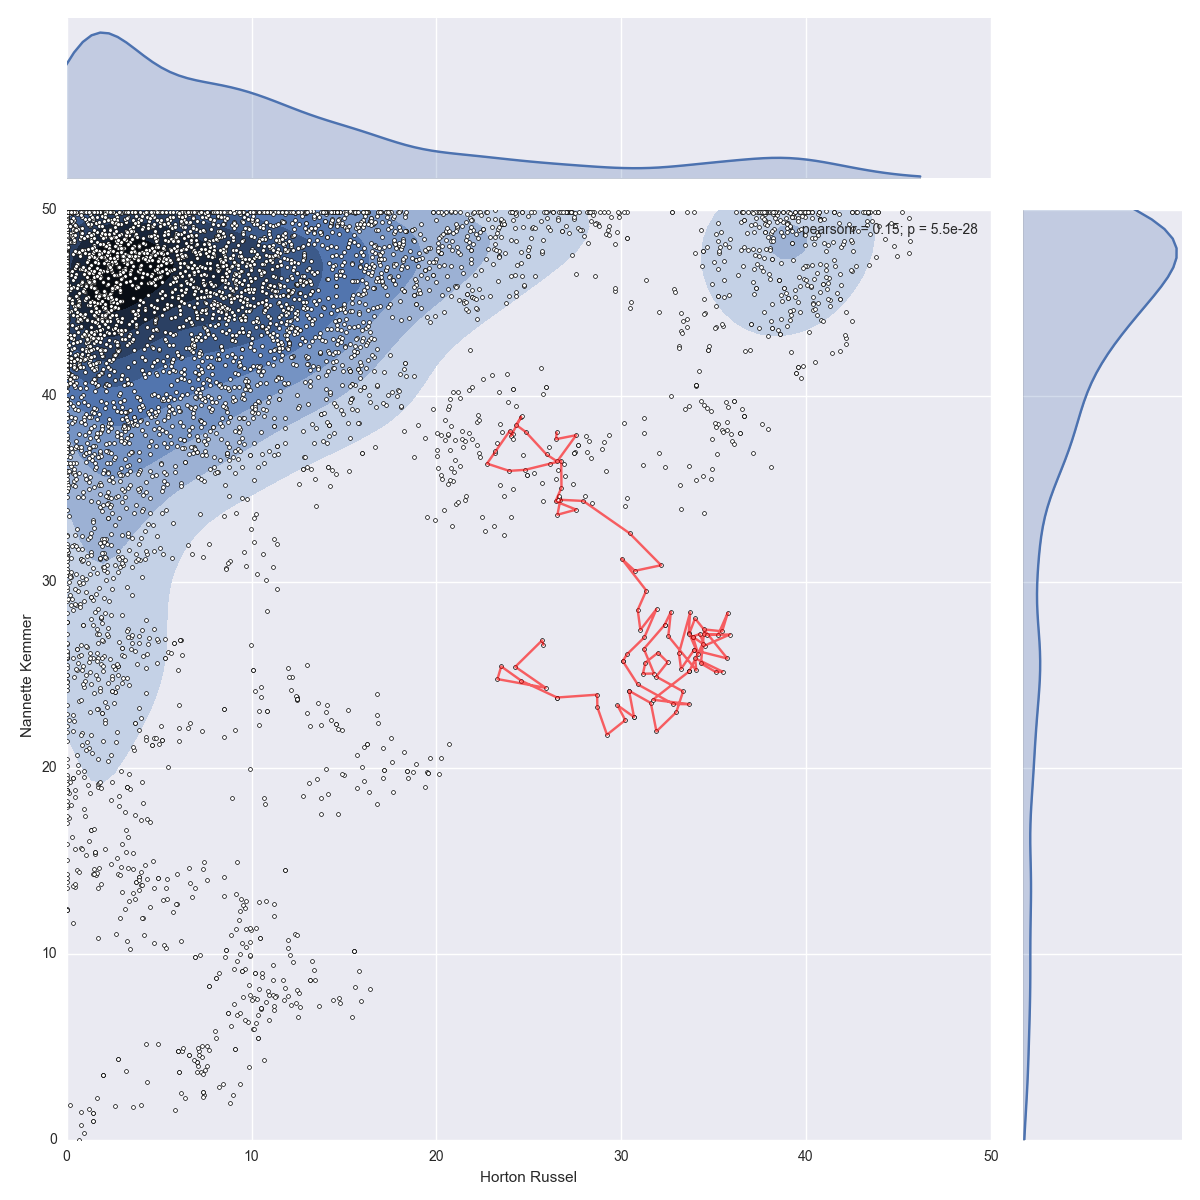
\includegraphics[width=0.7\columnwidth]{out/T8_23/MH/plot/joint_scatter_plot} \\
	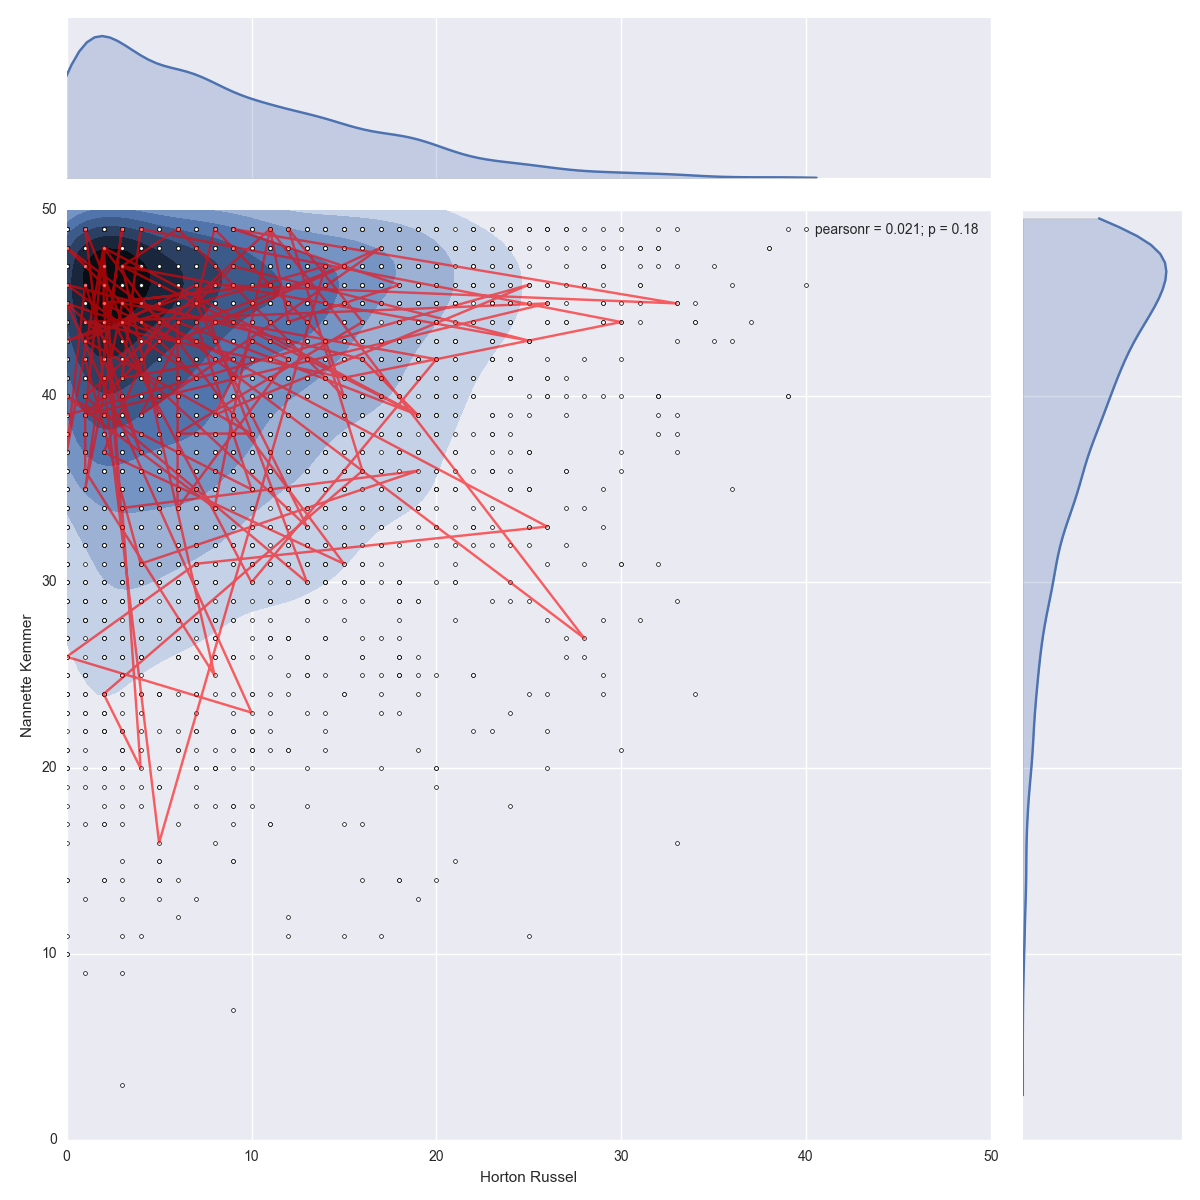
\includegraphics[width=0.7\columnwidth]{out/T8_23/Gibbs/plot/joint_scatter_plot} \\
	\caption{First 100 samples from Metropolis-Hastings algorithm (above), and Gibbs Sampler (below)}
	\label{dmaçsd}
\end{figure}
\begin{table}
	\centering
	\caption{\textbf{Test 0}: MH. Good Acceptance/Rejection ratio. Space is explored well.}
	\csvautotabular[respect underscore]{img/out/T8_23/MH/csv/1_signature.csv} \\[5mm]
	\csvautotabular[respect sharp]{img/out/T8_23/MH/csv/2_reel_skills.csv} %
	\csvautotabular[respect sharp]{img/out/T8_23/MH/csv/3_skills.csv} \\[5mm]
	\csvautotabular[respect sharp]{img/out/T8_23/MH/csv/7_errors.csv} \hspace{3mm}% 
	\csvautotabular[respect sharp]{img/out/T8_23/MH/csv/5_correct_incorrect.csv} \\[5mm]	
	\csvautotabular[respect sharp]{img/out/T8_23/MH/csv/6_errors.csv} \\[5mm]
	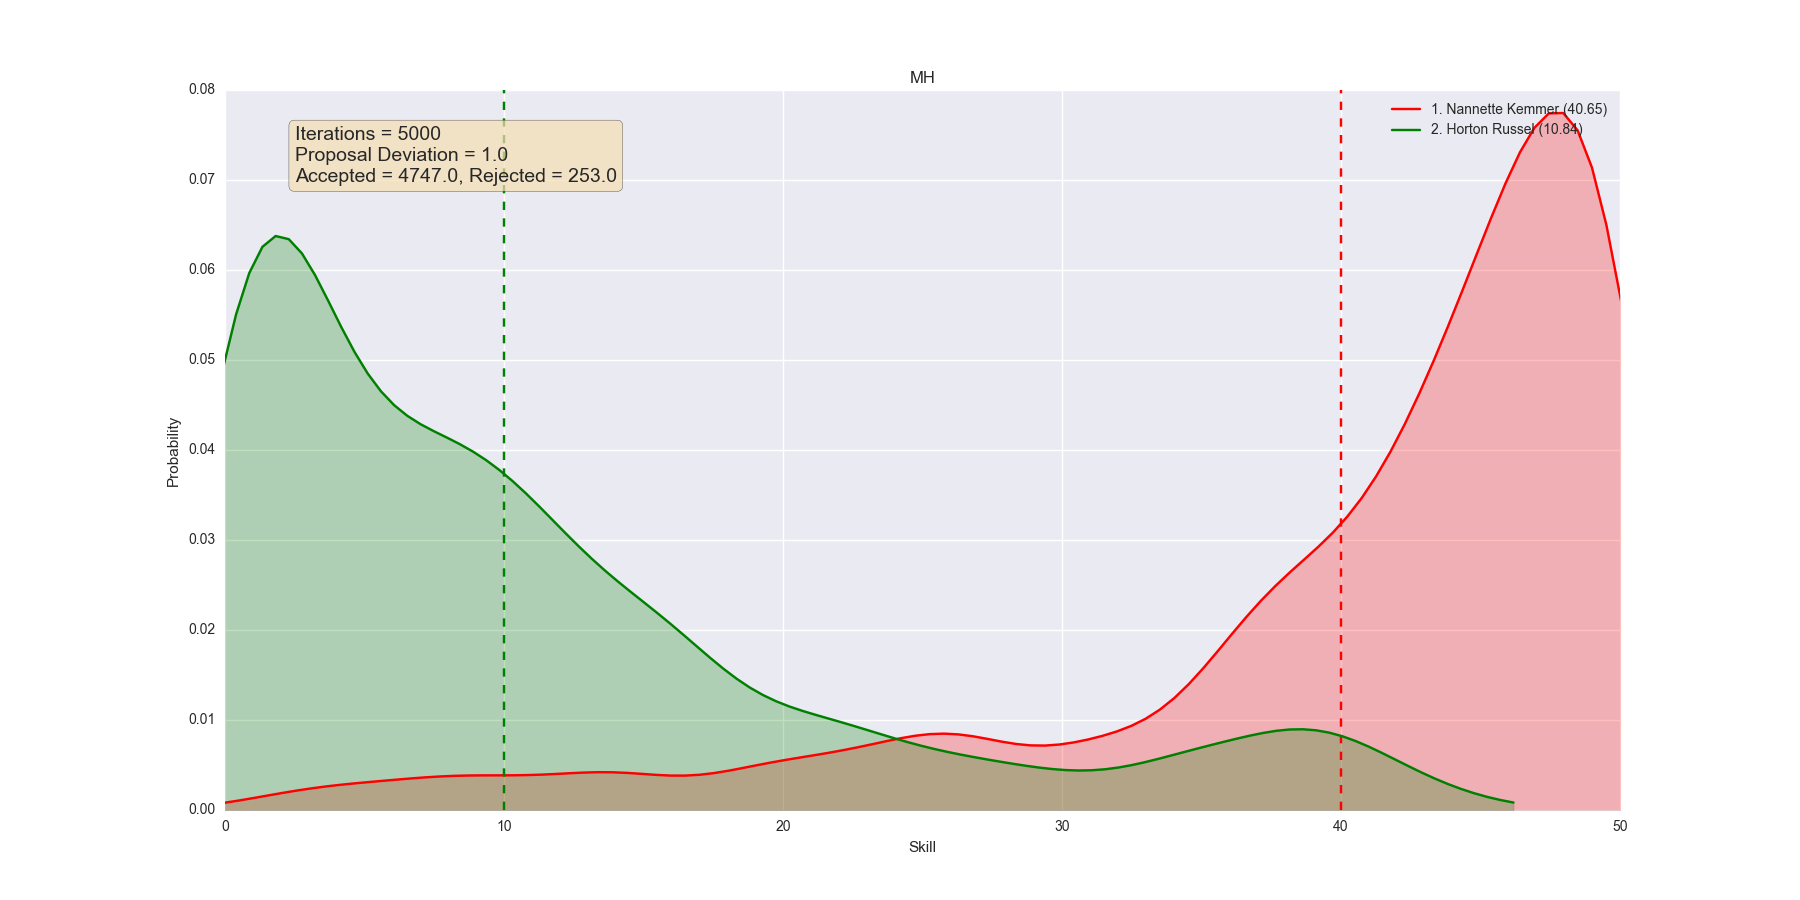
\includegraphics[width=1\columnwidth]{out/T8_23/MH/plot/skill_distribution}
\end{table}
\begin{table}
	\centering
	\caption{\textbf{Test 0:} Gibbs sampler. Accurate result.}
	\csvautotabular[respect underscore]{img/out/T8_23/Gibbs/csv/1_signature.csv} \\[5mm]
	\csvautotabular[respect sharp]{img/out/T8_23/Gibbs/csv/2_reel_skills.csv} %
	\csvautotabular[respect sharp]{img/out/T8_23/Gibbs/csv/3_skills.csv} \\[5mm]
	\csvautotabular[respect sharp]{img/out/T8_23/Gibbs/csv/7_errors.csv} \hspace{3mm}% 
	\csvautotabular[respect sharp]{img/out/T8_23/Gibbs/csv/5_correct_incorrect.csv} \\[5mm]	
	\csvautotabular[respect sharp]{img/out/T8_23/Gibbs/csv/6_errors.csv} \\[5mm]
	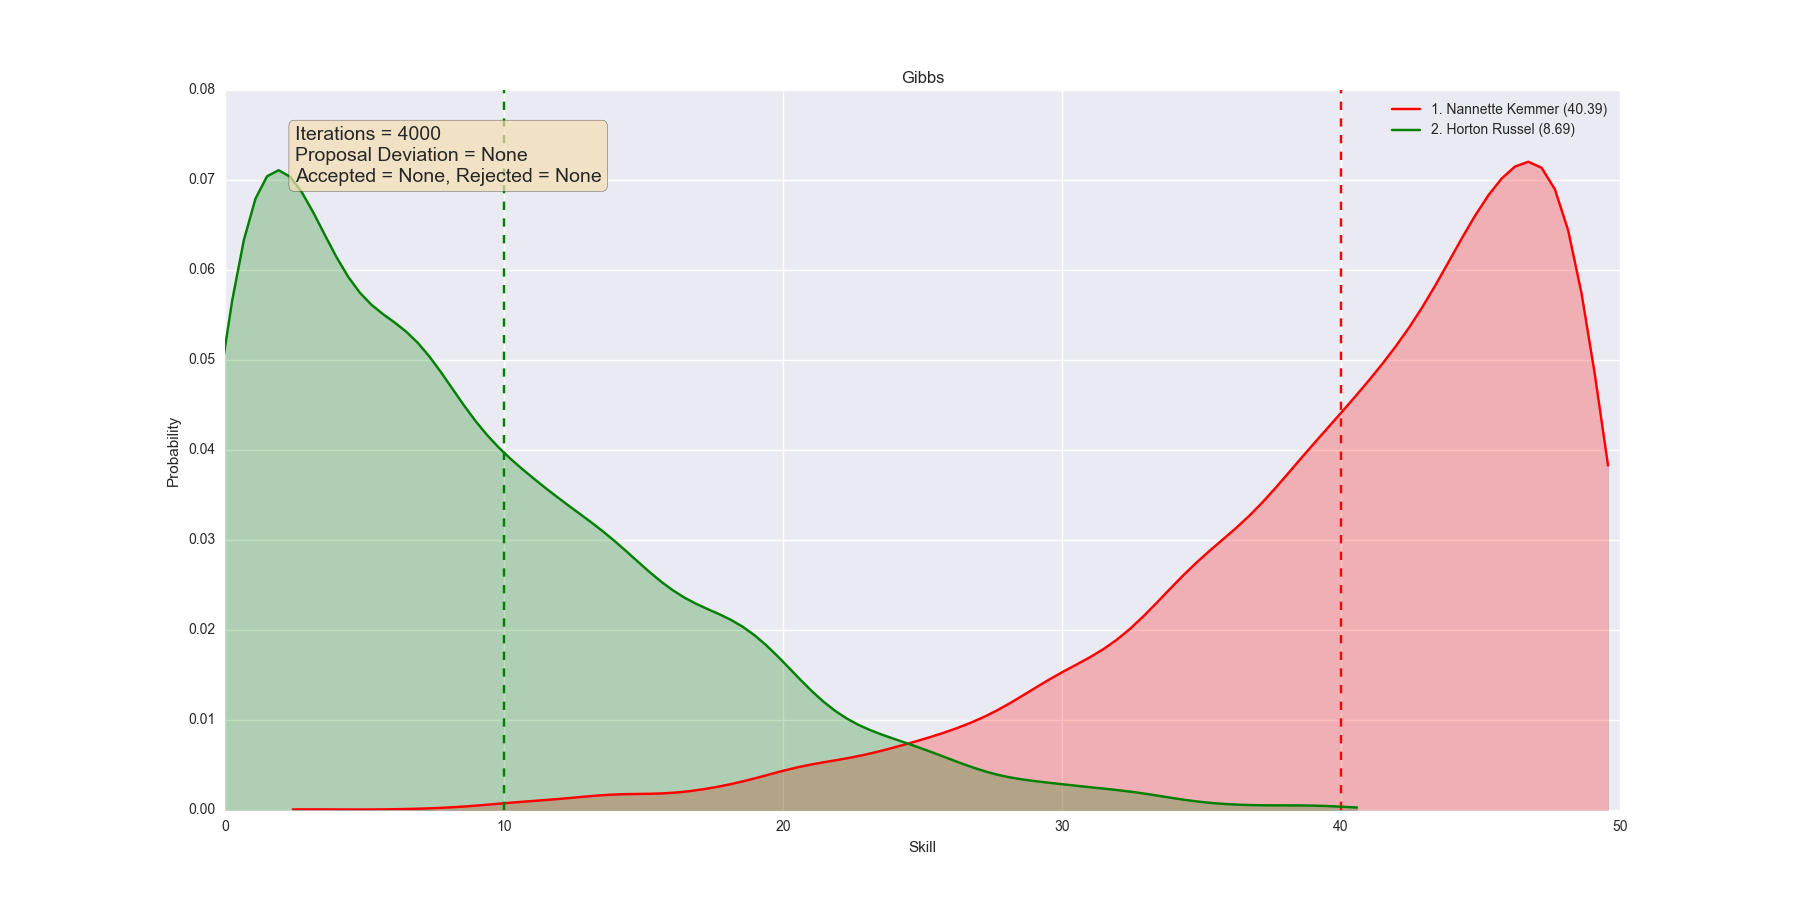
\includegraphics[width=1\columnwidth]{out/T8_23/Gibbs/plot/skill_distribution} \\
\end{table}
\begin{table}
	\centering
	\caption{\textbf{Test 0:} EP}
	\csvautotabular[respect underscore]{img/out/T8_23/EP/csv/1_signature.csv} \\[5mm]
	\csvautotabular[respect sharp]{img/out/T8_23/EP/csv/2_reel_skills.csv} %
	\csvautotabular[respect sharp]{img/out/T8_23/EP/csv/3_skills.csv} \\[5mm]
	\csvautotabular[respect sharp]{img/out/T8_23/EP/csv/7_errors.csv} \hspace{3mm}% 
	\csvautotabular[respect sharp]{img/out/T8_23/EP/csv/5_correct_incorrect.csv} \\[5mm]	
	\csvautotabular[respect sharp]{img/out/T8_23/EP/csv/6_errors.csv} \\[5mm]
	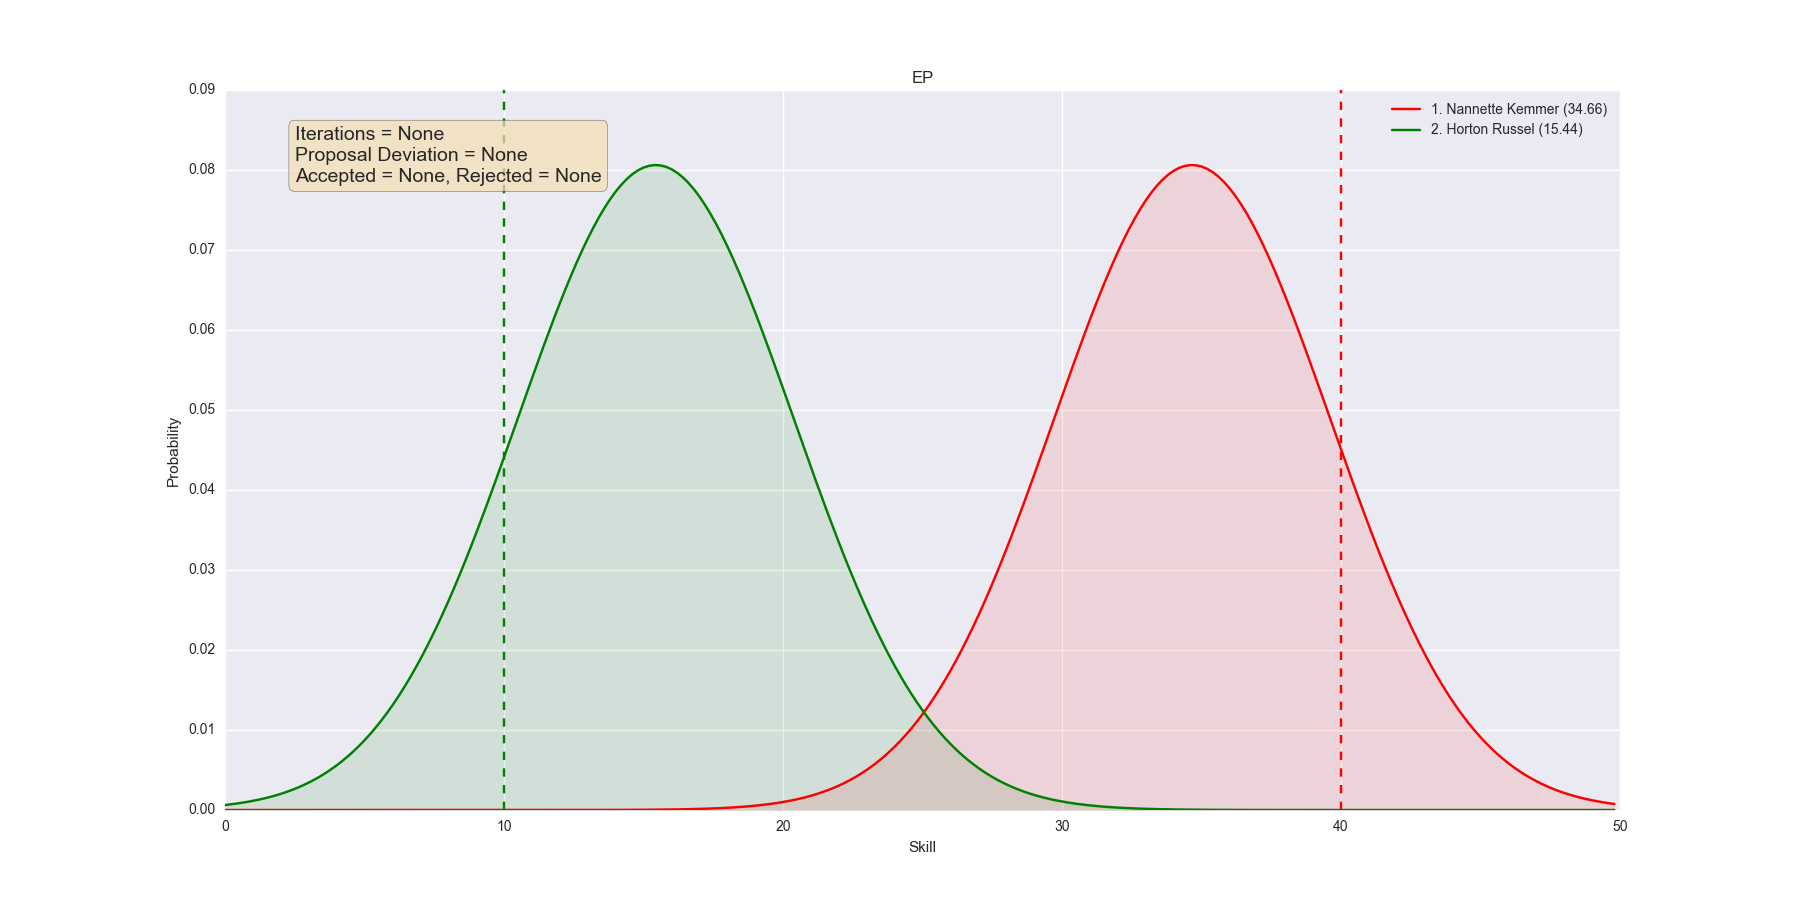
\includegraphics[width=1\columnwidth]{out/T8_23/EP/plot/skill_distribution} \\
\end{table}




\clearpage
\begin{table}
	\centering
	\singlespacing
	\tabcolsep=0.11cm
	\caption{\textbf{Test 1.1}: MH. Large number of matches result in accurate predictions.}
	\csvautotabular[respect underscore]{img/out/T1_1_Wed/MH/csv/1_signature.csv} \\[5mm]
	\csvautotabular[respect sharp]{img/out/T1_1_Wed/MH/csv/2_reel_skills.csv} %
	\csvautotabular[respect sharp]{img/out/T1_1_Wed/MH/csv/3_skills.csv} \\[5mm]
	\csvautotabular[respect sharp]{img/out/T1_1_Wed/MH/csv/7_errors.csv} \hspace{3mm}% 
	\csvautotabular[respect sharp]{img/out/T1_1_Wed/MH/csv/5_correct_incorrect.csv} \\[5mm]	
	\csvautotabular[respect sharp]{img/out/T1_1_Wed/MH/csv/6_errors.csv} \\[5mm]
	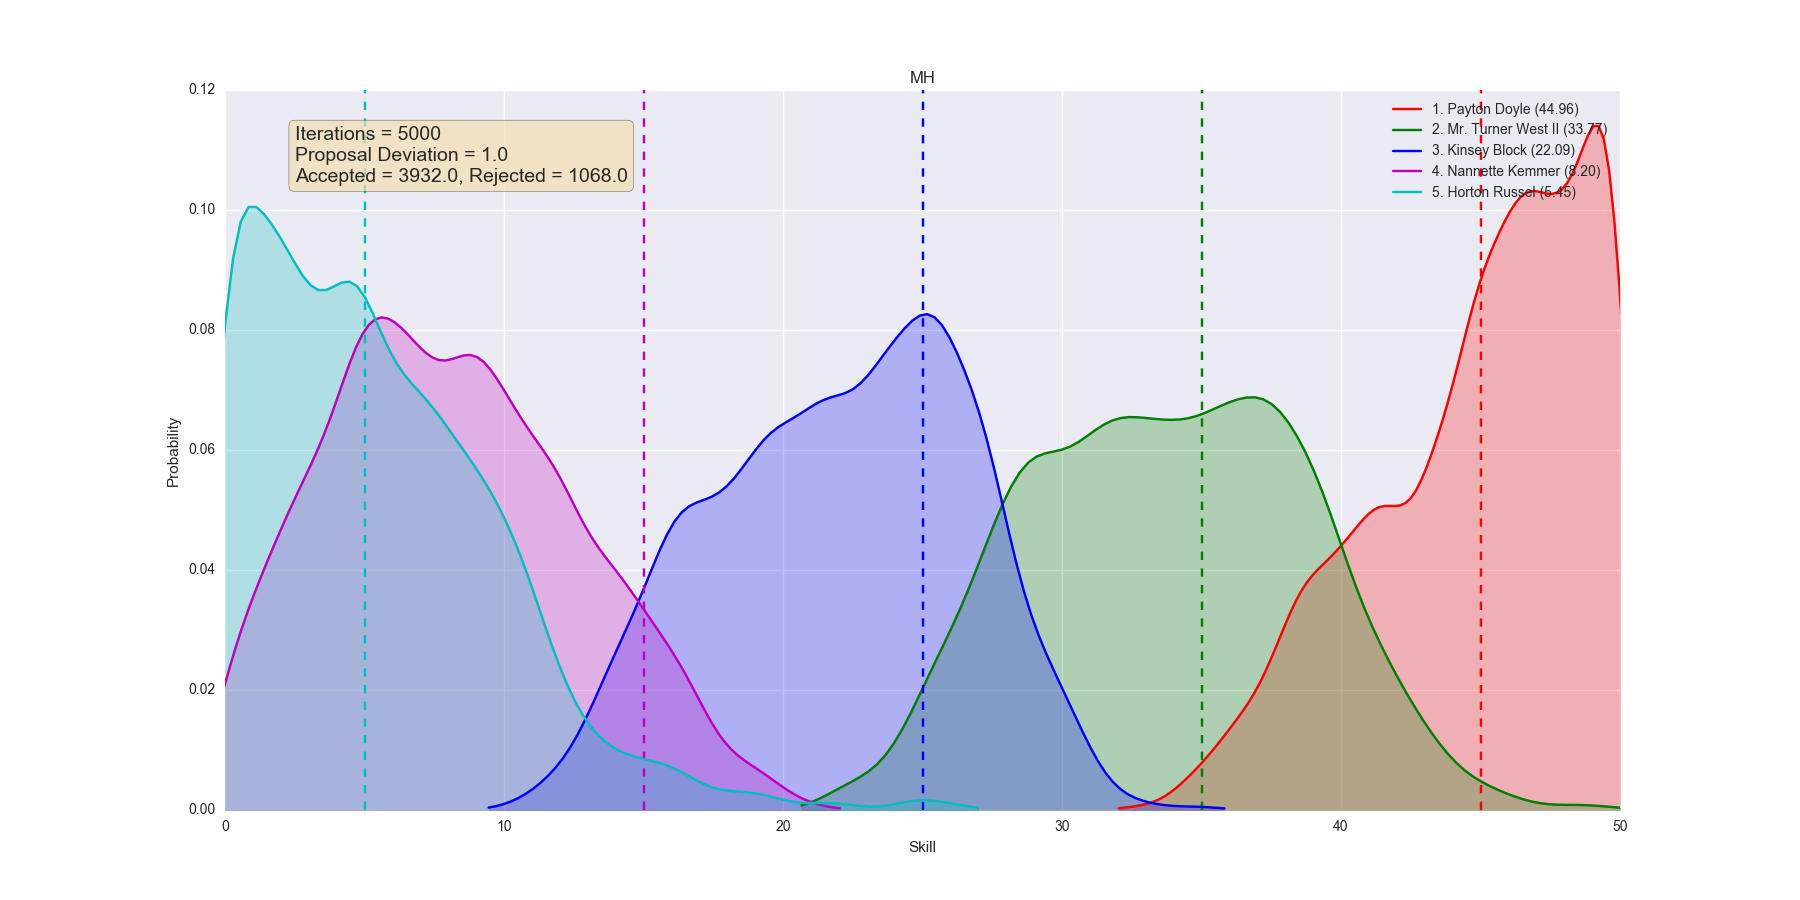
\includegraphics[width=1\columnwidth]{out/T1_1_Wed/MH/plot/skill_distribution}
\end{table}
\begin{table}
	\centering
	\singlespacing
	\tabcolsep=0.11cm
	\caption{\textbf{Test 1.1}}
	\csvautotabular[respect underscore]{img/out/T1_1_Wed/Gibbs/csv/1_signature.csv} \\[5mm]
	\csvautotabular[respect sharp]{img/out/T1_1_Wed/Gibbs/csv/2_reel_skills.csv} %
	\csvautotabular[respect sharp]{img/out/T1_1_Wed/Gibbs/csv/3_skills.csv} \\[5mm]
	\csvautotabular[respect sharp]{img/out/T1_1_Wed/Gibbs/csv/7_errors.csv} \hspace{3mm}% 
	\csvautotabular[respect sharp]{img/out/T1_1_Wed/Gibbs/csv/5_correct_incorrect.csv} \\[5mm]	
	\csvautotabular[respect sharp]{img/out/T1_1_Wed/Gibbs/csv/6_errors.csv} \\[5mm]
	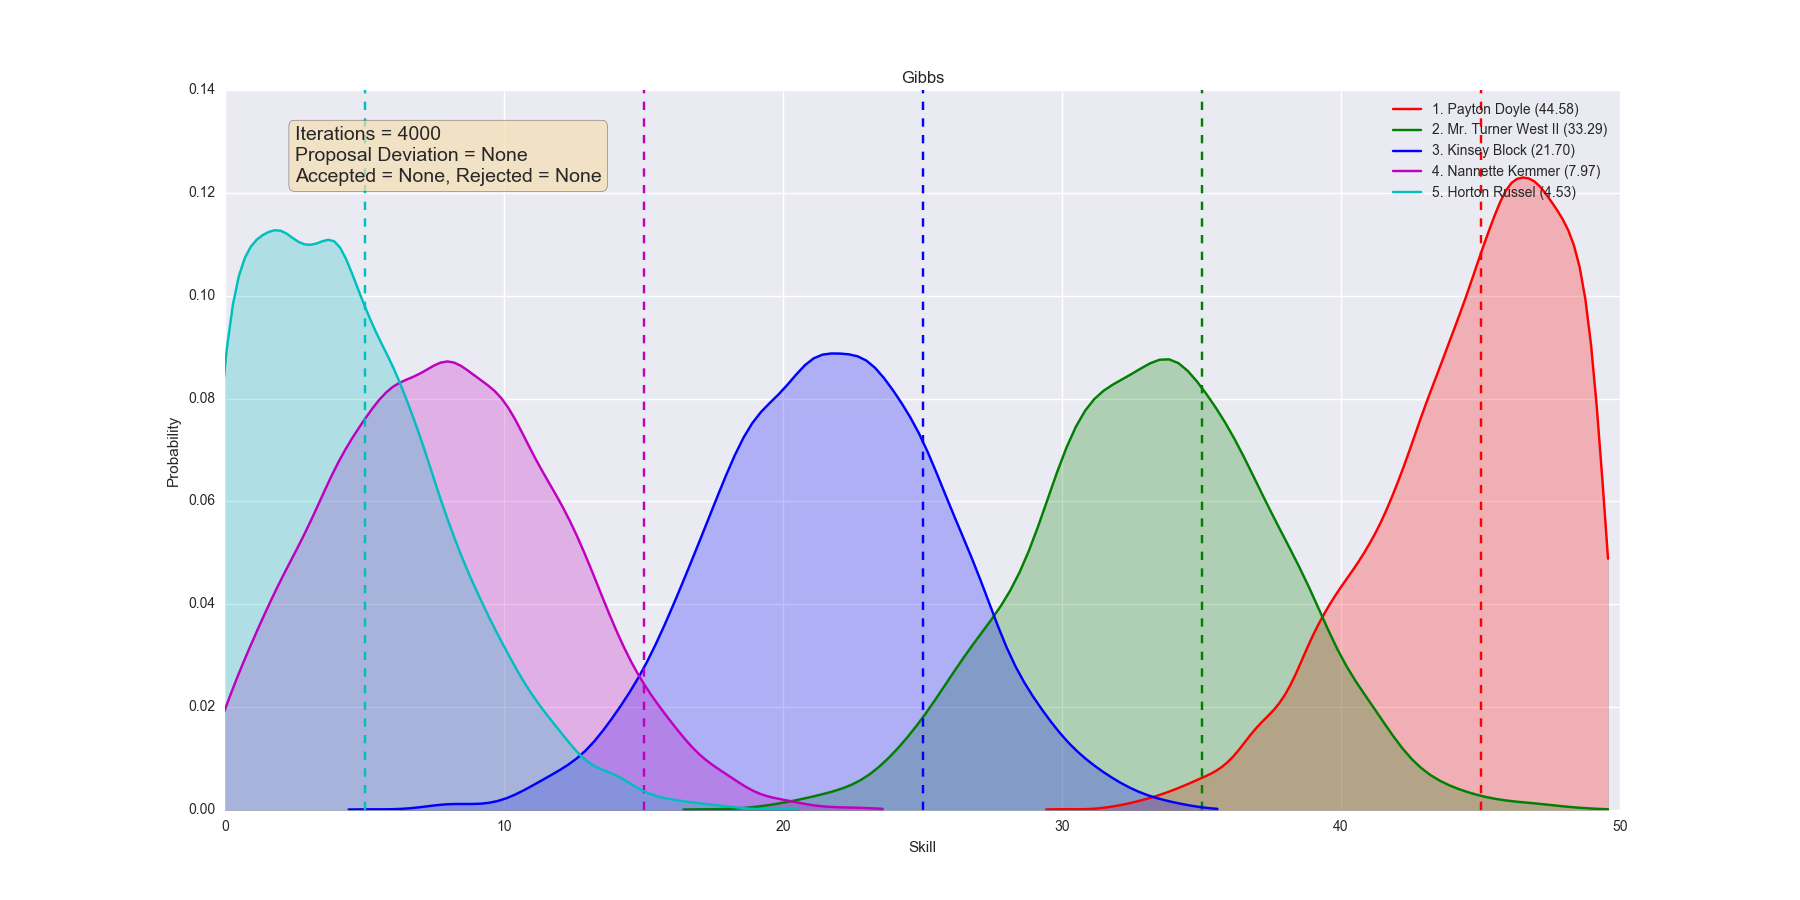
\includegraphics[width=1\columnwidth]{out/T1_1_Wed/Gibbs/plot/skill_distribution} \\
\end{table}
\begin{table}
	\centering
	\singlespacing
	\tabcolsep=0.11cm
	\caption{\textbf{Test 1.1}}
	\csvautotabular[respect underscore]{img/out/T1_1_Wed/EP/csv/1_signature.csv} \\[5mm]
	\csvautotabular[respect sharp]{img/out/T1_1_Wed/EP/csv/2_reel_skills.csv} %
	\csvautotabular[respect sharp]{img/out/T1_1_Wed/EP/csv/3_skills.csv} \\[5mm]
	\csvautotabular[respect sharp]{img/out/T1_1_Wed/EP/csv/7_errors.csv} \hspace{3mm}% 
	\csvautotabular[respect sharp]{img/out/T1_1_Wed/EP/csv/5_correct_incorrect.csv} \\[5mm]	
	\csvautotabular[respect sharp]{img/out/T1_1_Wed/EP/csv/6_errors.csv} \\[5mm]
	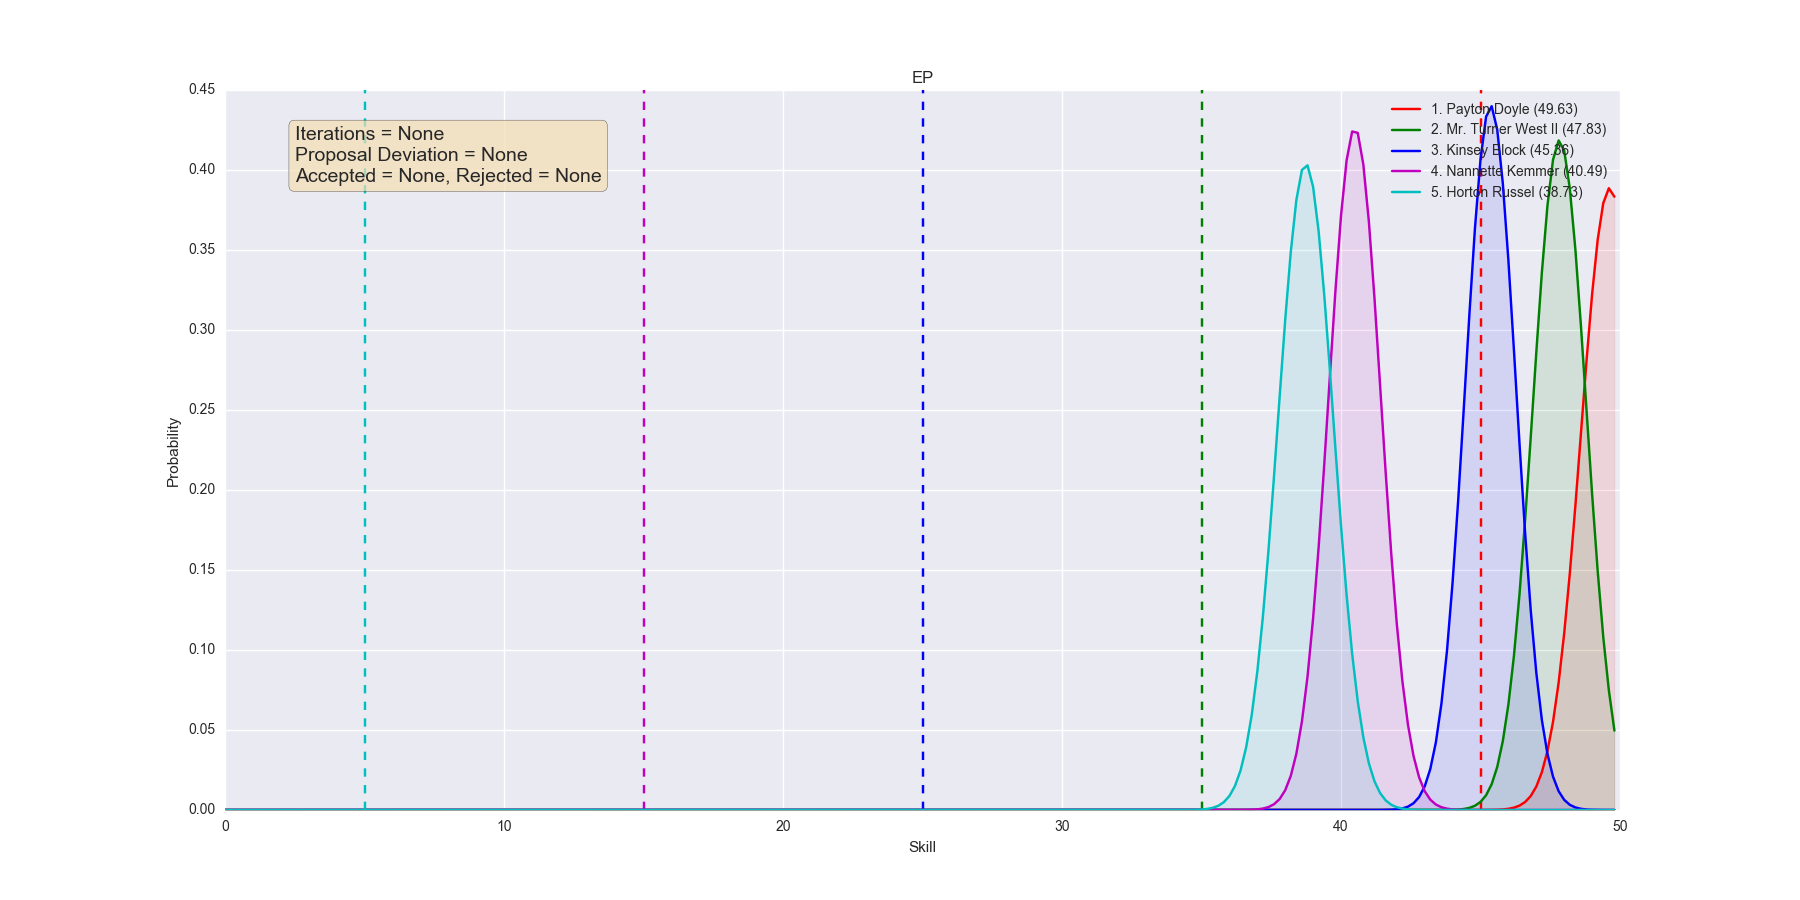
\includegraphics[width=1\columnwidth]{out/T1_1_Wed/EP/plot/skill_distribution} \\
\end{table}



\clearpage
\begin{table}
	\centering
	\caption{\textbf{Test 1.2}}
	\csvautotabular[respect underscore]{img/out/T1_5/MH/csv/1_signature.csv} \\[5mm]
	\csvautotabular[respect sharp]{img/out/T1_5/MH/csv/2_reel_skills.csv} %
	\csvautotabular[respect sharp]{img/out/T1_5/MH/csv/3_skills.csv} \\[5mm]
	\csvautotabular[respect sharp]{img/out/T1_5/MH/csv/7_errors.csv} \hspace{3mm}% 
	\csvautotabular[respect sharp]{img/out/T1_5/MH/csv/5_correct_incorrect.csv} \\[5mm]	
	\csvautotabular[respect sharp]{img/out/T1_5/MH/csv/6_errors.csv} \\[5mm]
	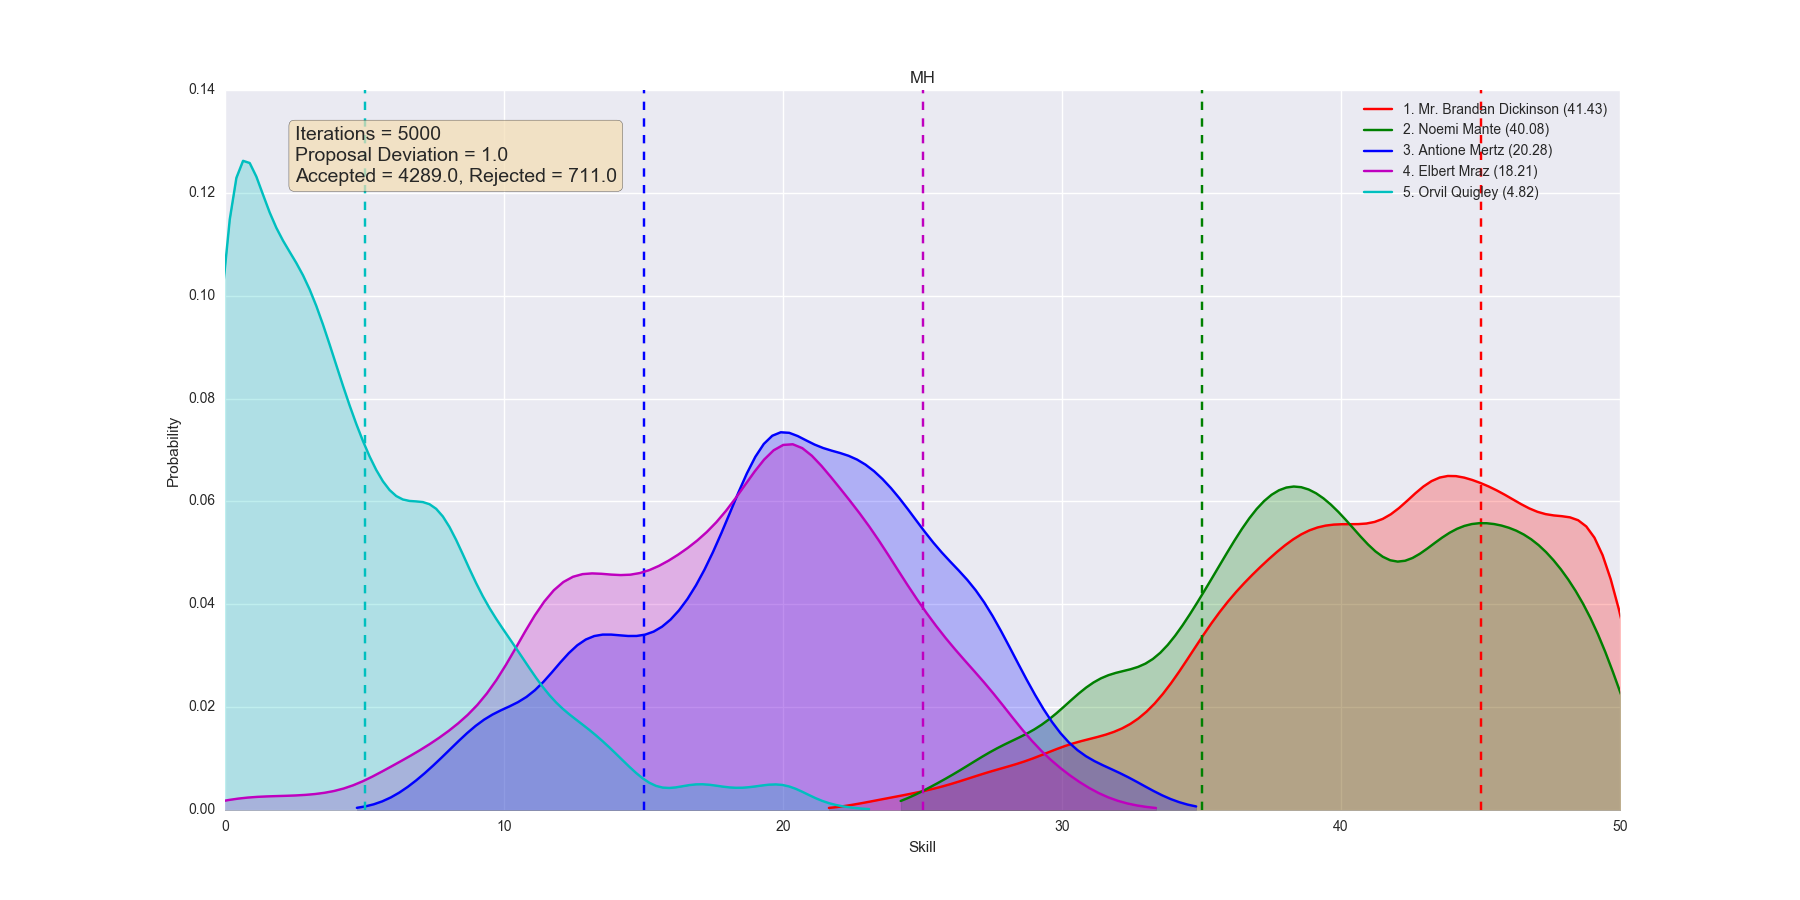
\includegraphics[width=1\columnwidth]{out/T1_5/MH/plot/skill_distribution}
\end{table}
\begin{table}
	\centering
	\caption{\textbf{Test 1.2}}
	\csvautotabular[respect underscore]{img/out/T1_5/Gibbs/csv/1_signature.csv} \\[5mm]
	\csvautotabular[respect sharp]{img/out/T1_5/Gibbs/csv/2_reel_skills.csv} %
	\csvautotabular[respect sharp]{img/out/T1_5/Gibbs/csv/3_skills.csv} \\[5mm]
	\csvautotabular[respect sharp]{img/out/T1_5/Gibbs/csv/7_errors.csv} \hspace{3mm}% 
	\csvautotabular[respect sharp]{img/out/T1_5/Gibbs/csv/5_correct_incorrect.csv} \\[5mm]	
	\csvautotabular[respect sharp]{img/out/T1_5/Gibbs/csv/6_errors.csv} \\[5mm]
	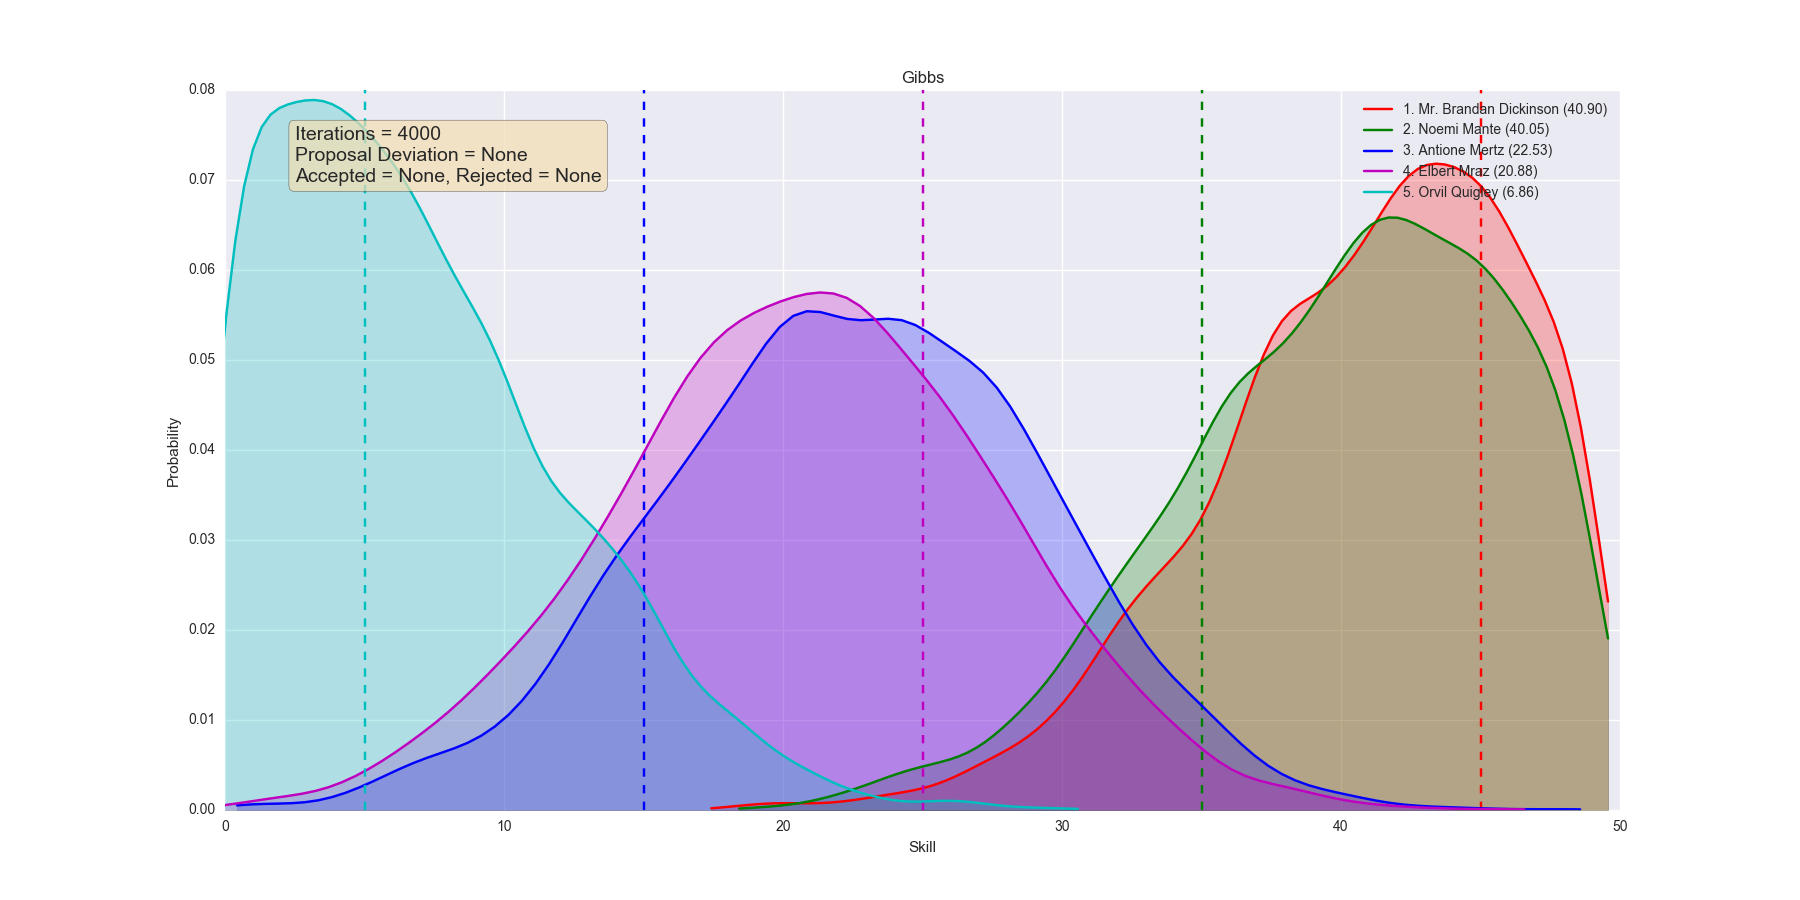
\includegraphics[width=1\columnwidth]{out/T1_5/Gibbs/plot/skill_distribution} \\
\end{table}
\begin{table}
	\centering
	\caption{\textbf{Test 1.2}}
	\csvautotabular[respect underscore]{img/out/T1_5/EP/csv/1_signature.csv} \\[5mm]
	\csvautotabular[respect sharp]{img/out/T1_5/EP/csv/2_reel_skills.csv} %
	\csvautotabular[respect sharp]{img/out/T1_5/EP/csv/3_skills.csv} \\[5mm]
	\csvautotabular[respect sharp]{img/out/T1_5/EP/csv/7_errors.csv} \hspace{3mm}% 
	\csvautotabular[respect sharp]{img/out/T1_5/EP/csv/5_correct_incorrect.csv} \\[5mm]	
	\csvautotabular[respect sharp]{img/out/T1_5/EP/csv/6_errors.csv} \\[5mm]
	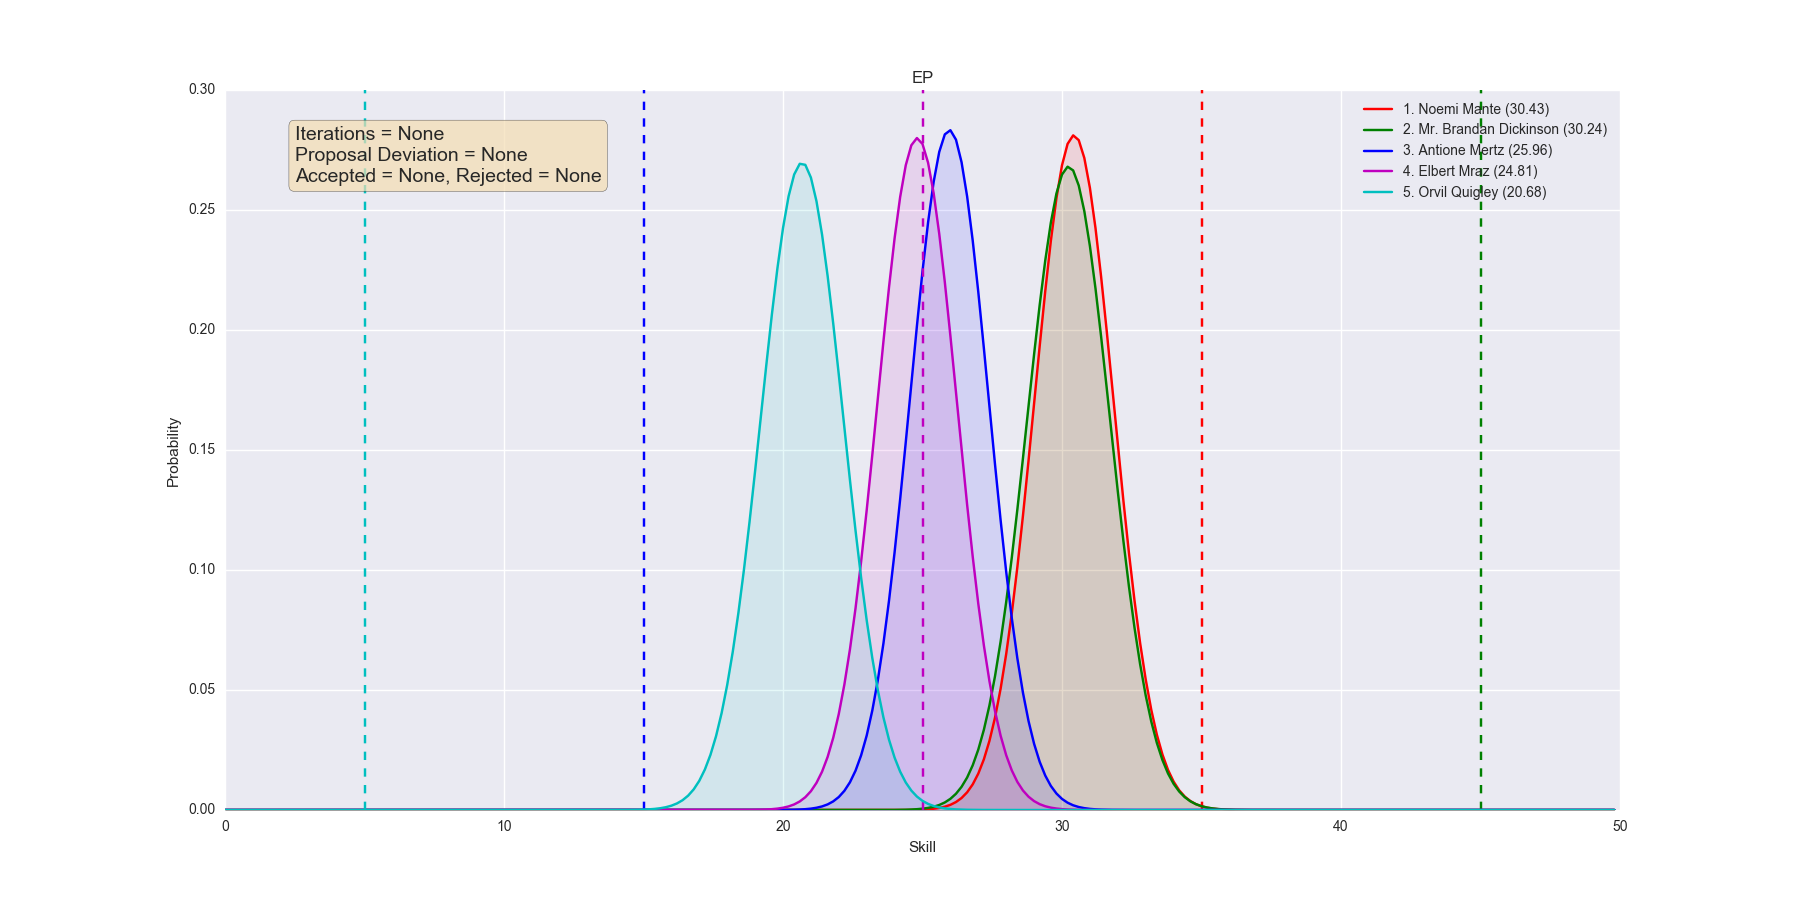
\includegraphics[width=1\columnwidth]{out/T1_5/EP/plot/skill_distribution} \\
\end{table}



\clearpage
\begin{table}
	\centering
	\caption{\textbf{Test 2}}
	\csvautotabular[respect underscore]{img/out/T2_7_Wed/MH/csv/1_signature.csv} \\[5mm]
	\csvautotabular[respect sharp]{img/out/T2_7_Wed/MH/csv/2_reel_skills.csv} %
	\csvautotabular[respect sharp]{img/out/T2_7_Wed/MH/csv/3_skills.csv} \\[5mm]
	\csvautotabular[respect sharp]{img/out/T2_7_Wed/MH/csv/7_errors.csv} \hspace{3mm}% 
	\csvautotabular[respect sharp]{img/out/T2_7_Wed/MH/csv/5_correct_incorrect.csv} \\[5mm]	
	\csvautotabular[respect sharp]{img/out/T2_7_Wed/MH/csv/6_errors.csv} \\[5mm]
	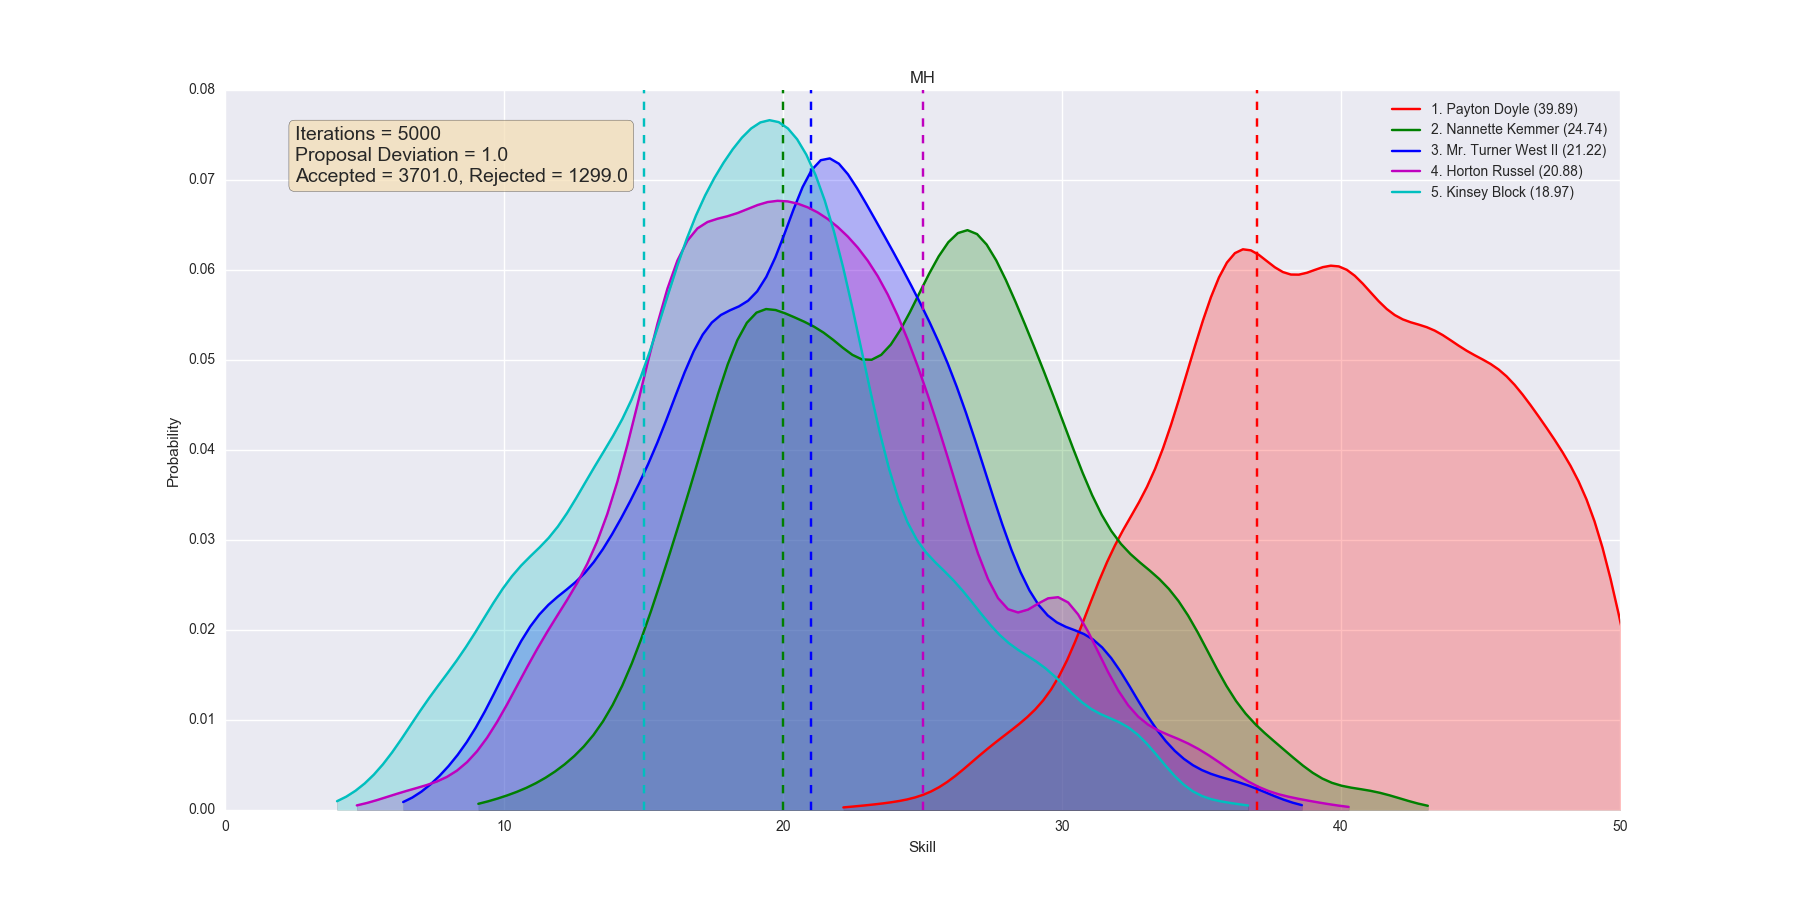
\includegraphics[width=1\columnwidth]{out/T2_7_Wed/MH/plot/skill_distribution}
\end{table}
\begin{table}
	\centering
	\caption{\textbf{Test 2}}
	\csvautotabular[respect underscore]{img/out/T2_7_Wed/Gibbs/csv/1_signature.csv} \\[5mm]
	\csvautotabular[respect sharp]{img/out/T2_7_Wed/Gibbs/csv/2_reel_skills.csv} %
	\csvautotabular[respect sharp]{img/out/T2_7_Wed/Gibbs/csv/3_skills.csv} \\[5mm]
	\csvautotabular[respect sharp]{img/out/T2_7_Wed/Gibbs/csv/7_errors.csv} \hspace{3mm}% 
	\csvautotabular[respect sharp]{img/out/T2_7_Wed/Gibbs/csv/5_correct_incorrect.csv} \\[5mm]	
	\csvautotabular[respect sharp]{img/out/T2_7_Wed/Gibbs/csv/6_errors.csv} \\[5mm]
	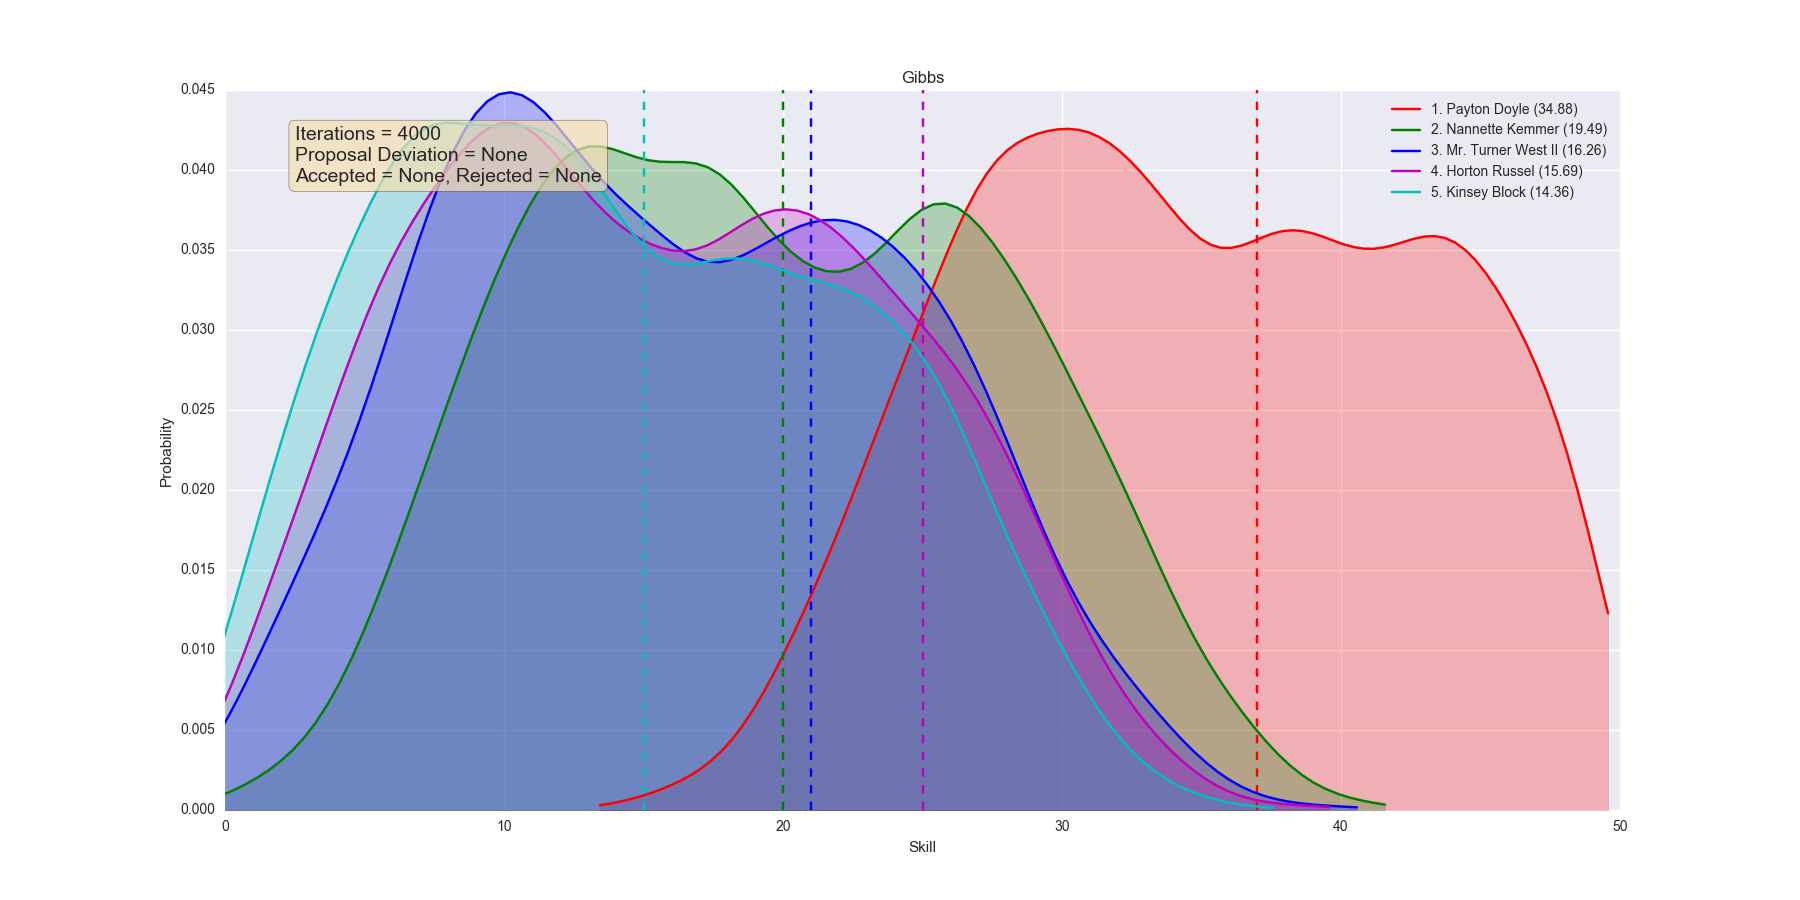
\includegraphics[width=1\columnwidth]{out/T2_7_Wed/Gibbs/plot/skill_distribution} \\
\end{table}
\begin{table}
	\centering
	\caption{\textbf{Test 2}}
	\csvautotabular[respect underscore]{img/out/T2_7/EP/csv/1_signature.csv} \\[5mm]
	\csvautotabular[respect sharp]{img/out/T2_7/EP/csv/2_reel_skills.csv} %
	\csvautotabular[respect sharp]{img/out/T2_7/EP/csv/3_skills.csv} \\[5mm]
	\csvautotabular[respect sharp]{img/out/T2_7/EP/csv/7_errors.csv} \hspace{3mm}% 
	\csvautotabular[respect sharp]{img/out/T2_7/EP/csv/5_correct_incorrect.csv} \\[5mm]	
	\csvautotabular[respect sharp]{img/out/T2_7/EP/csv/6_errors.csv} \\[5mm]
	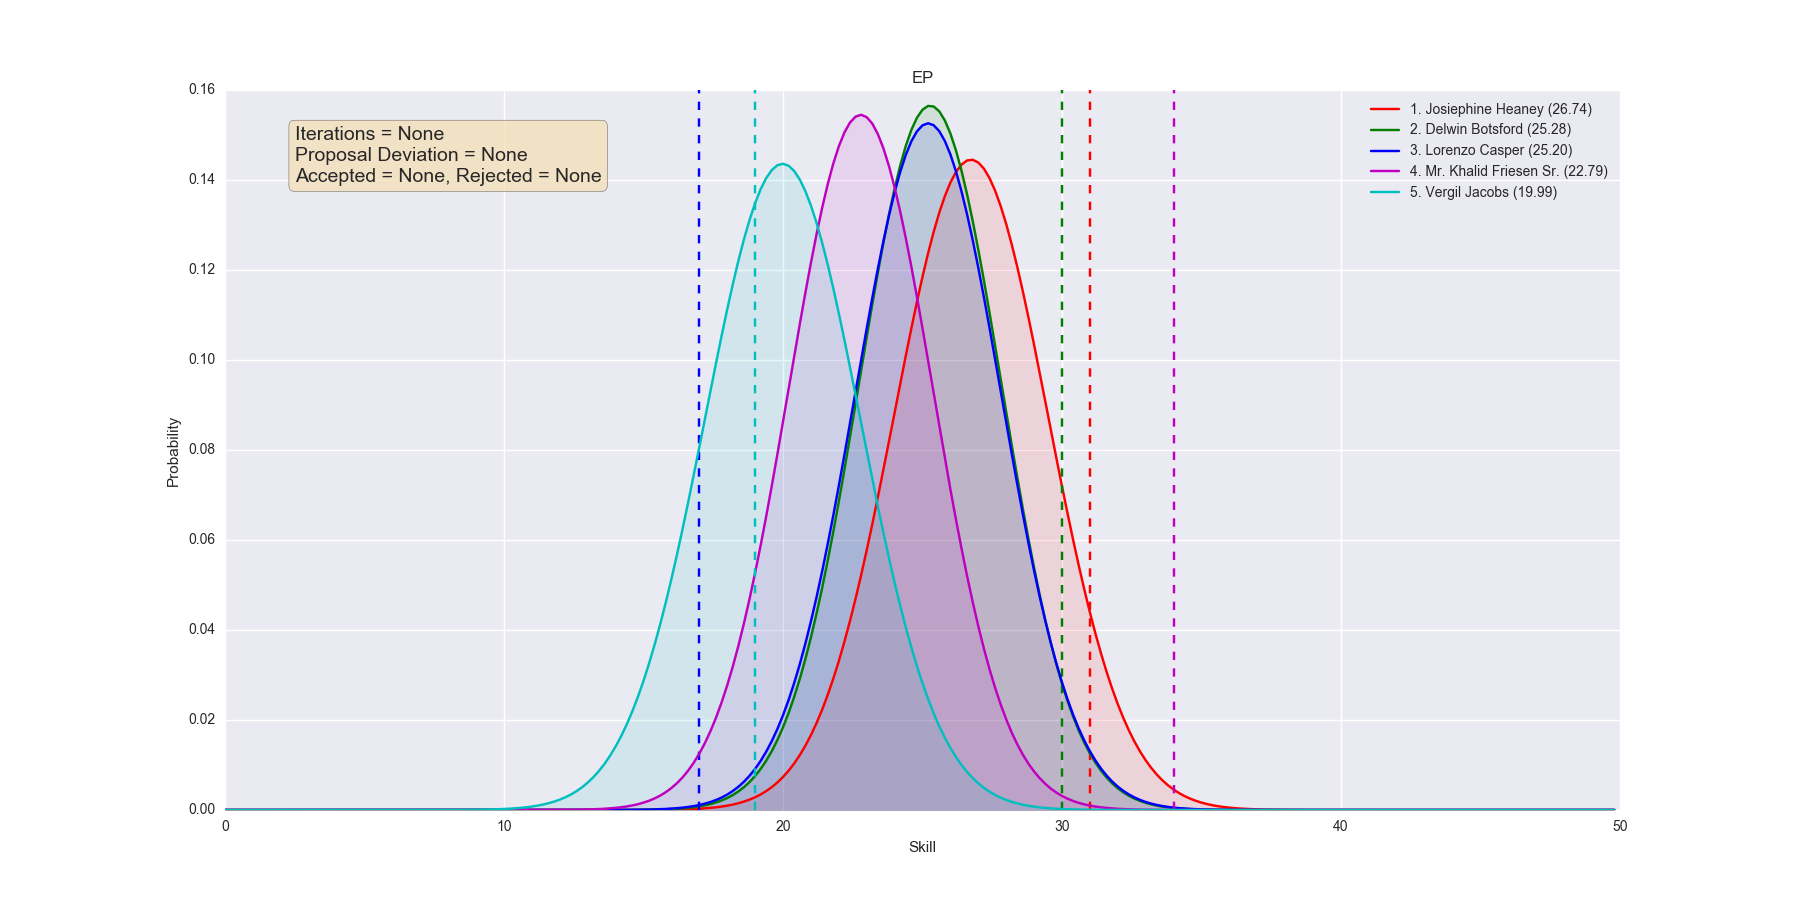
\includegraphics[width=1\columnwidth]{out/T2_7/EP/plot/skill_distribution} \\
\end{table}




\clearpage
\begin{table}
	\centering
	\caption{\textbf{Test 3.1}}
	\csvautotabular[respect underscore]{img/out/T3_9/MH/csv/1_signature.csv} \\[5mm]
	\csvautotabular[respect sharp]{img/out/T3_9/MH/csv/7_errors.csv} \hspace{3mm}% 
	\csvautotabular[respect sharp]{img/out/T3_9/MH/csv/5_correct_incorrect.csv} \\[5mm]	
	\csvautotabular[respect sharp]{img/out/T3_9/MH/csv/6_errors.csv} \\[5mm]
	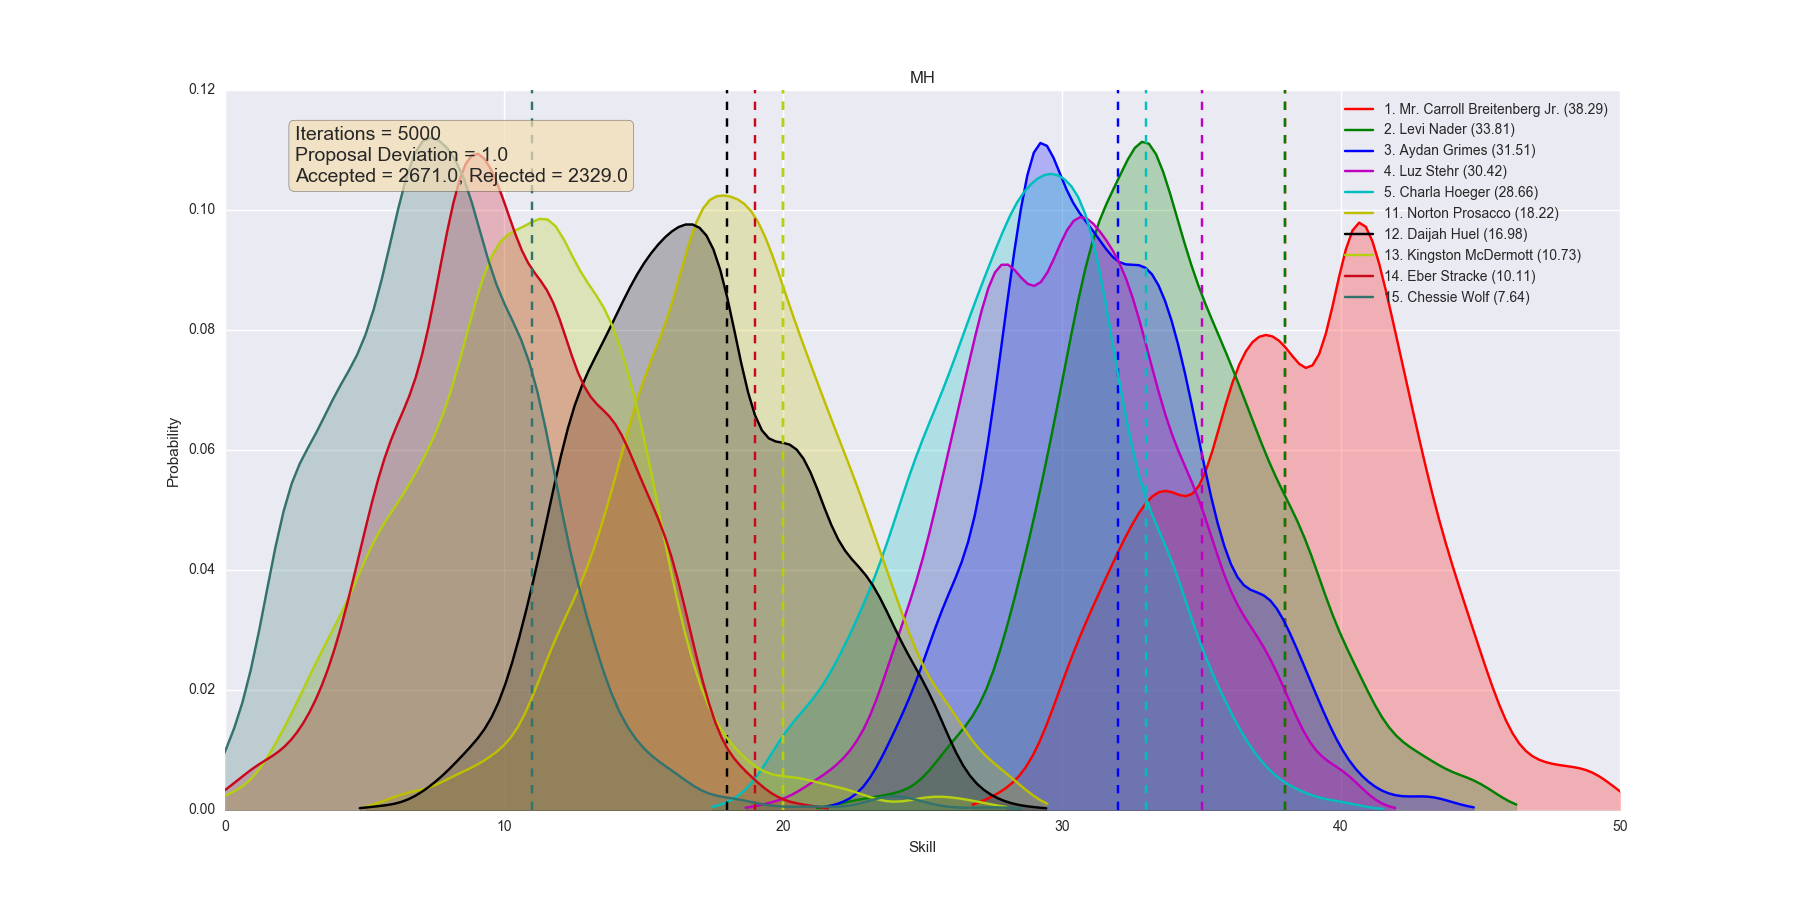
\includegraphics[width=1\columnwidth]{out/T3_9/MH/plot/skill_distribution}
\end{table}
\begin{table}
	\centering
	\caption{\textbf{Test 3.1}. As described in Section 5. There is no pivoting reel skills (close to 0 or 50) in this setup. Therefore there are uniques solutions. We observe shifted distributions.}
	\csvautotabular[respect underscore]{img/out/T3_9/Gibbs/csv/1_signature.csv} \\[5mm]
	\csvautotabular[respect sharp]{img/out/T3_9/Gibbs/csv/7_errors.csv} \hspace{3mm}% 
	\csvautotabular[respect sharp]{img/out/T3_9/Gibbs/csv/5_correct_incorrect.csv} \\[5mm]	
	\csvautotabular[respect sharp]{img/out/T3_9/Gibbs/csv/6_errors.csv} \\[5mm]
	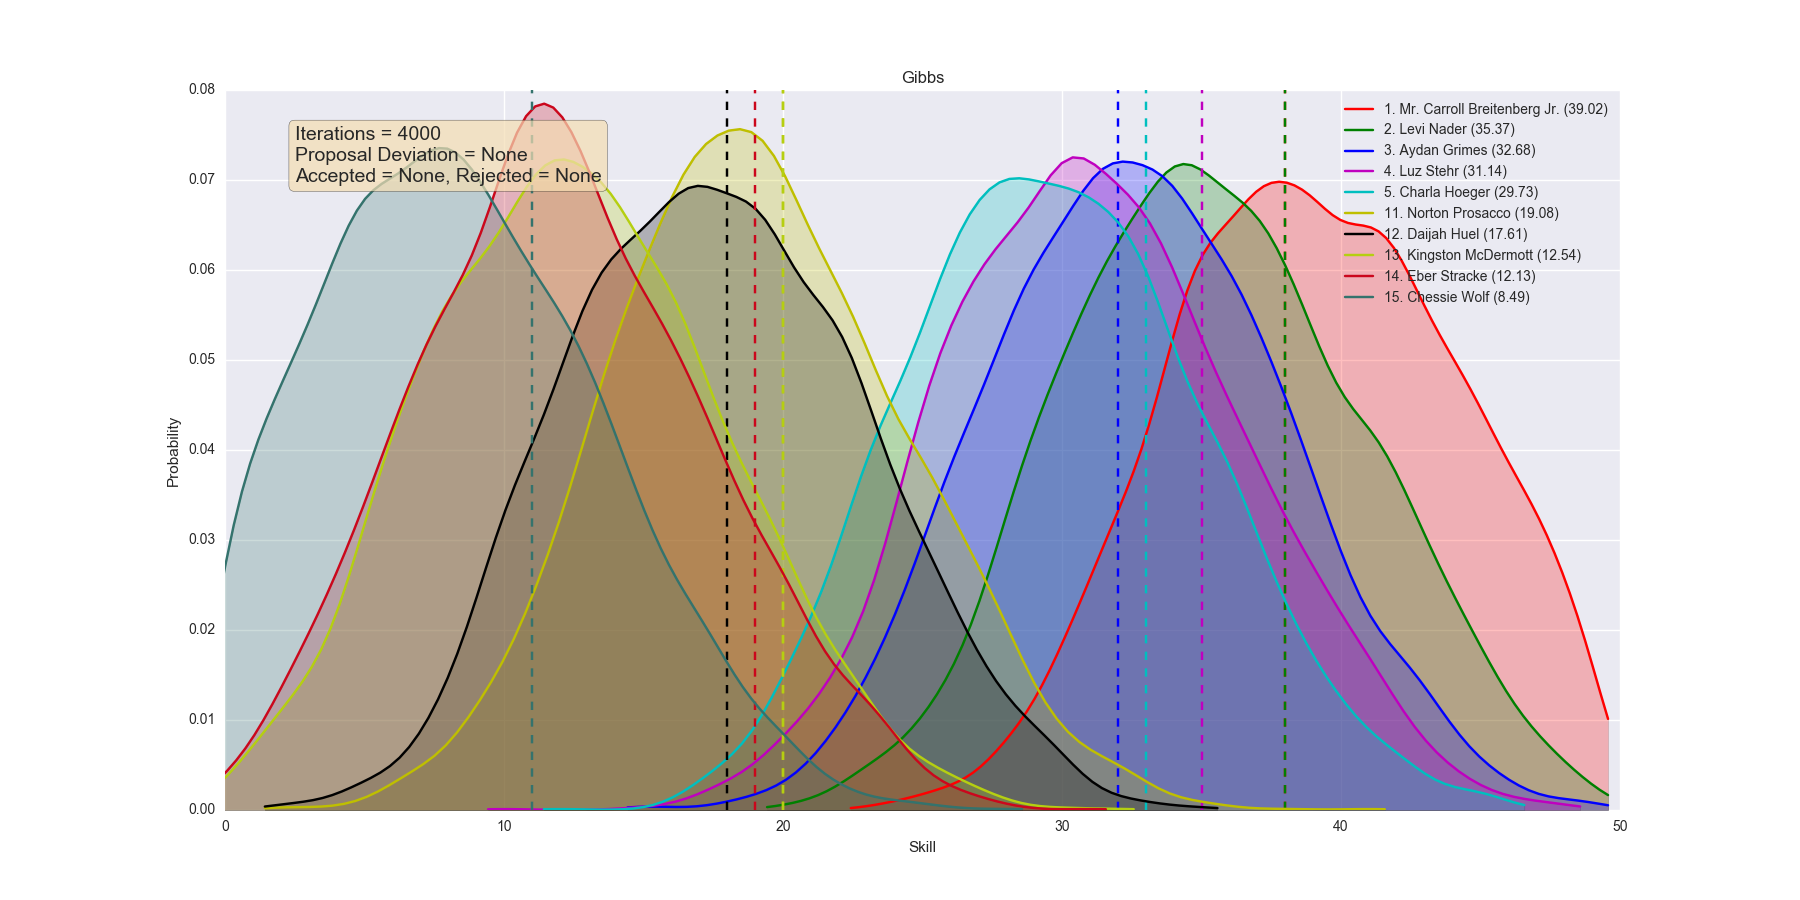
\includegraphics[width=1\columnwidth]{out/T3_9/Gibbs/plot/skill_distribution} \\
\end{table}



\clearpage
\begin{table}
	\centering
	\caption{\textbf{Test 4}}
	\csvautotabular[respect underscore]{img/out/T4_11/MH/csv/1_signature.csv} \\[5mm]
	\csvautotabular[respect sharp]{img/out/T4_11/MH/csv/7_errors.csv} \hspace{3mm}% 
	\csvautotabular[respect sharp]{img/out/T4_11/MH/csv/5_correct_incorrect.csv} \\[5mm]	
	\csvautotabular[respect sharp]{img/out/T4_11/MH/csv/6_errors.csv} \\[5mm]
	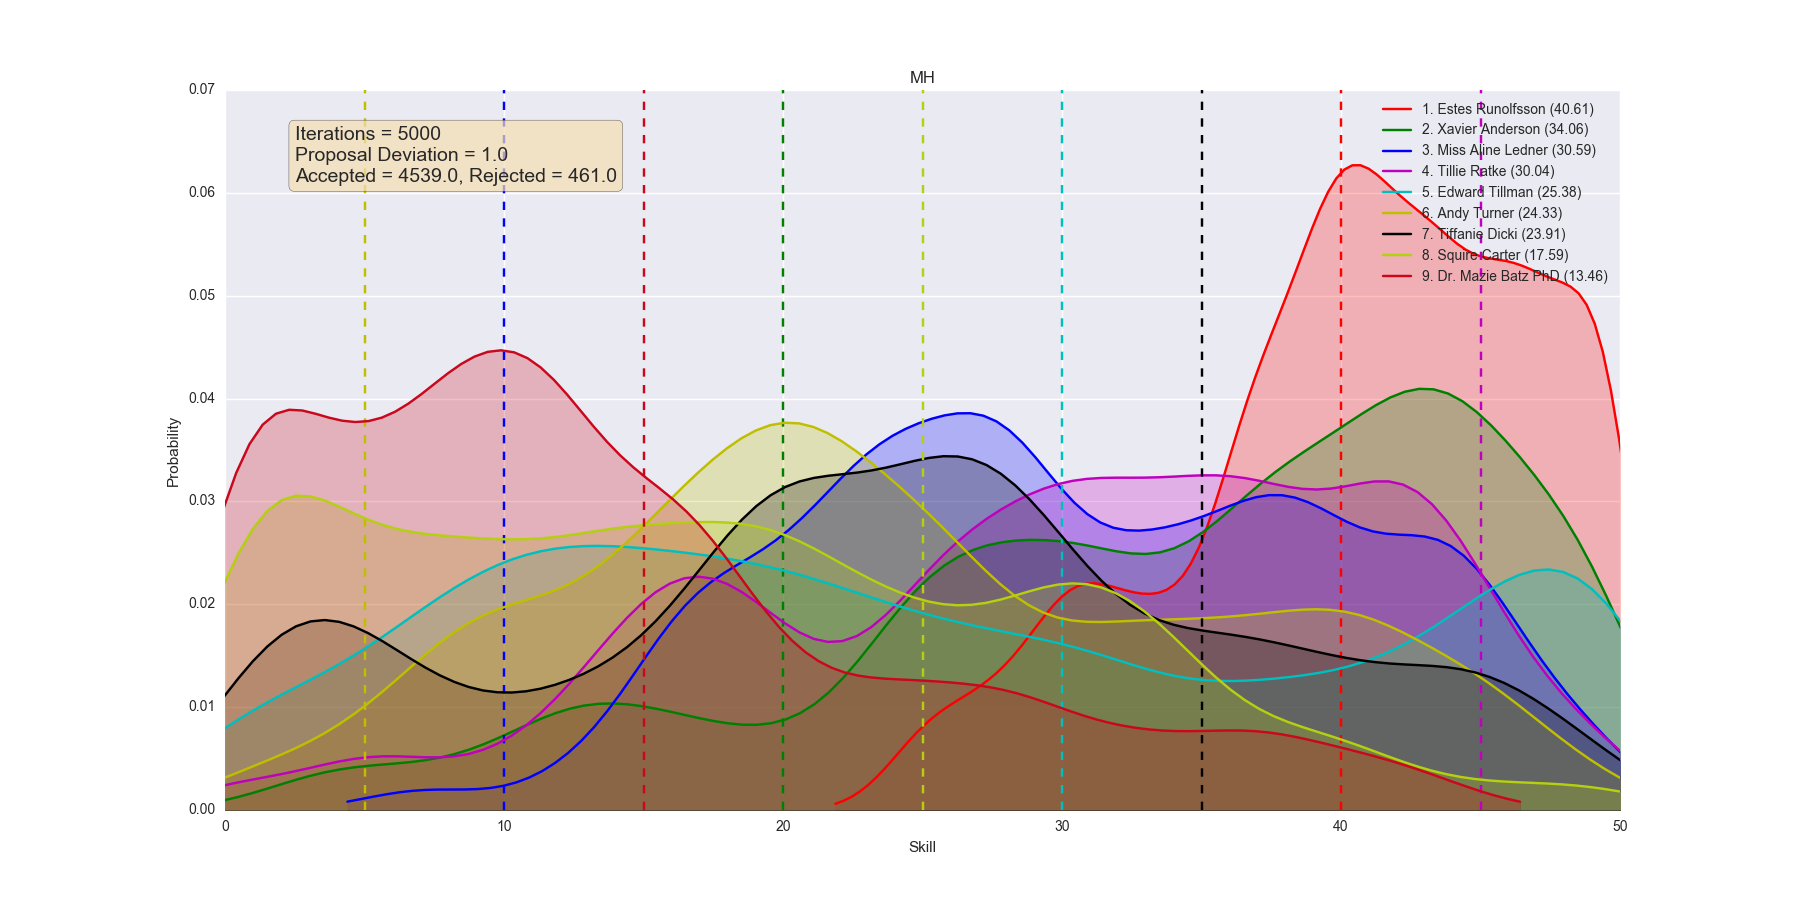
\includegraphics[width=1\columnwidth]{out/T4_11/MH/plot/skill_distribution}
\end{table}
\begin{table}
	\centering
	\caption{\textbf{Test 4}}
	\csvautotabular[respect underscore]{img/out/T4_11/Gibbs/csv/1_signature.csv} \\[5mm]
	\csvautotabular[respect sharp]{img/out/T4_11/Gibbs/csv/7_errors.csv} \hspace{3mm}% 
	\csvautotabular[respect sharp]{img/out/T4_11/Gibbs/csv/5_correct_incorrect.csv} \\[5mm]	
	\csvautotabular[respect sharp]{img/out/T4_11/Gibbs/csv/6_errors.csv} \\[5mm]
	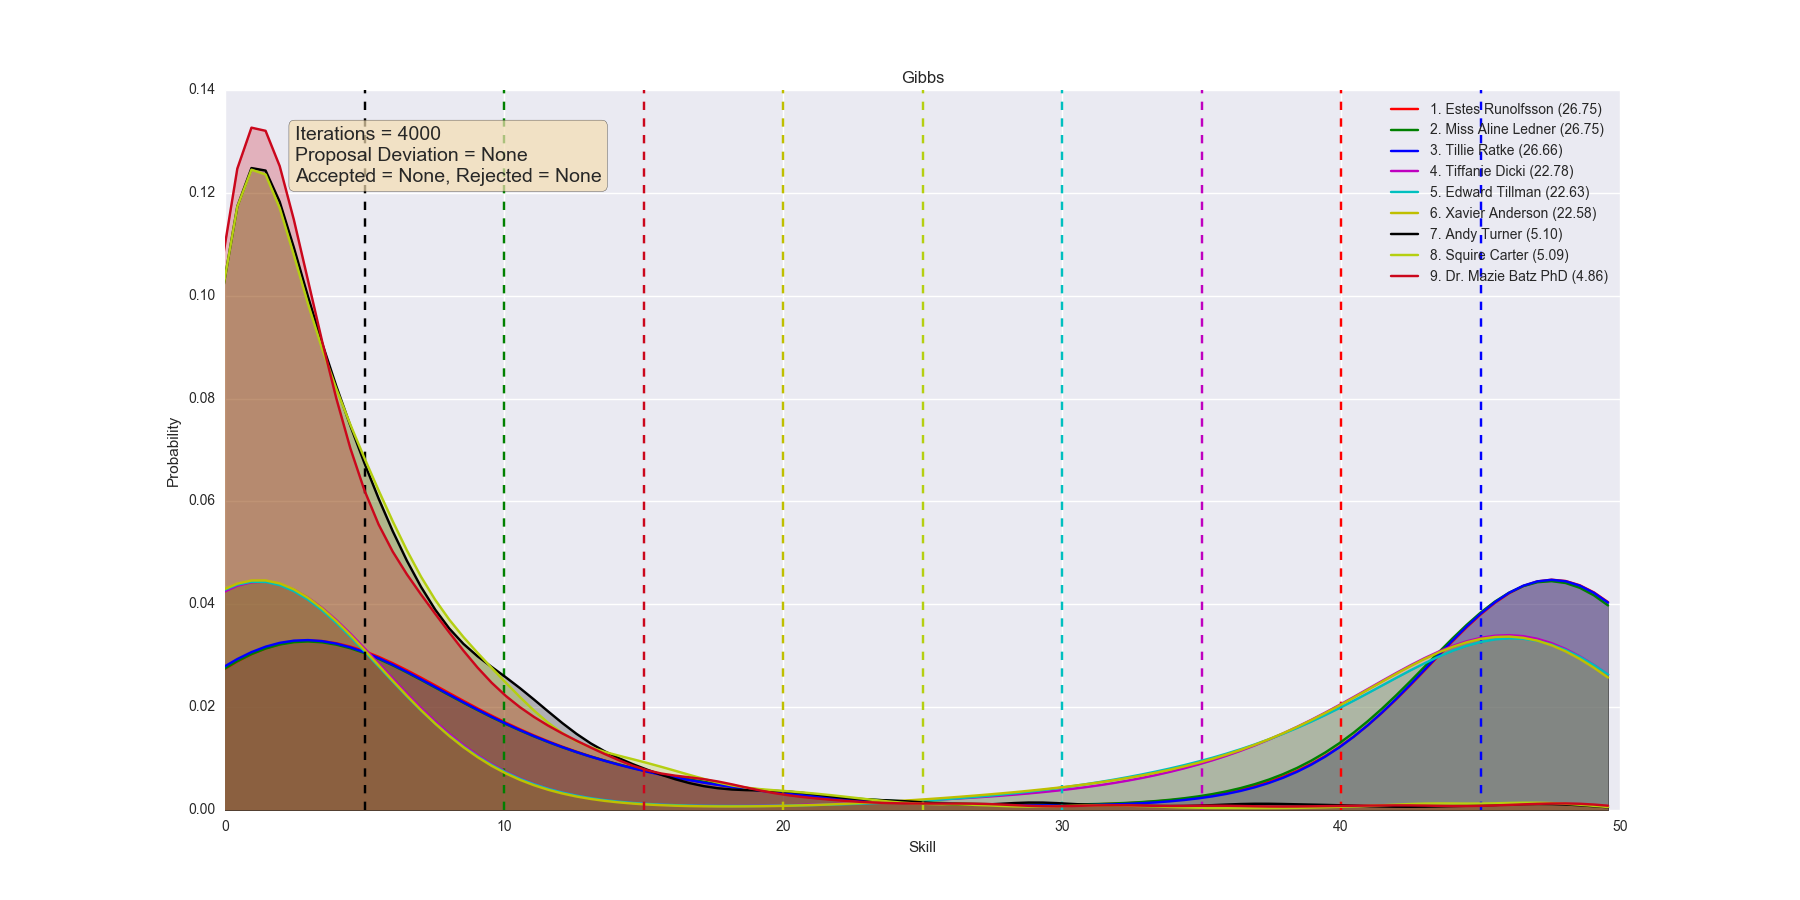
\includegraphics[width=1\columnwidth]{out/T4_11/Gibbs/plot/skill_distribution} \\
\end{table}



\clearpage
\begin{table}
	\small
	\centering
	\caption{\textbf{Test 5.1}}
	\csvautotabular[respect underscore]{img/out/T5_13/MH/csv/1_signature.csv} \\[5mm]
	\csvautotabular[respect sharp]{img/out/T5_13/MH/csv/3_skills_copy.csv} \hspace{3mm} %
	\csvautotabular[respect sharp]{img/out/T5_13/MH/csv/5_correct_incorrect.csv} \\[5mm]	
	\csvautotabular[respect sharp]{img/out/T5_13/MH/csv/4_predictions_copy.csv} \hspace{3mm}% 
	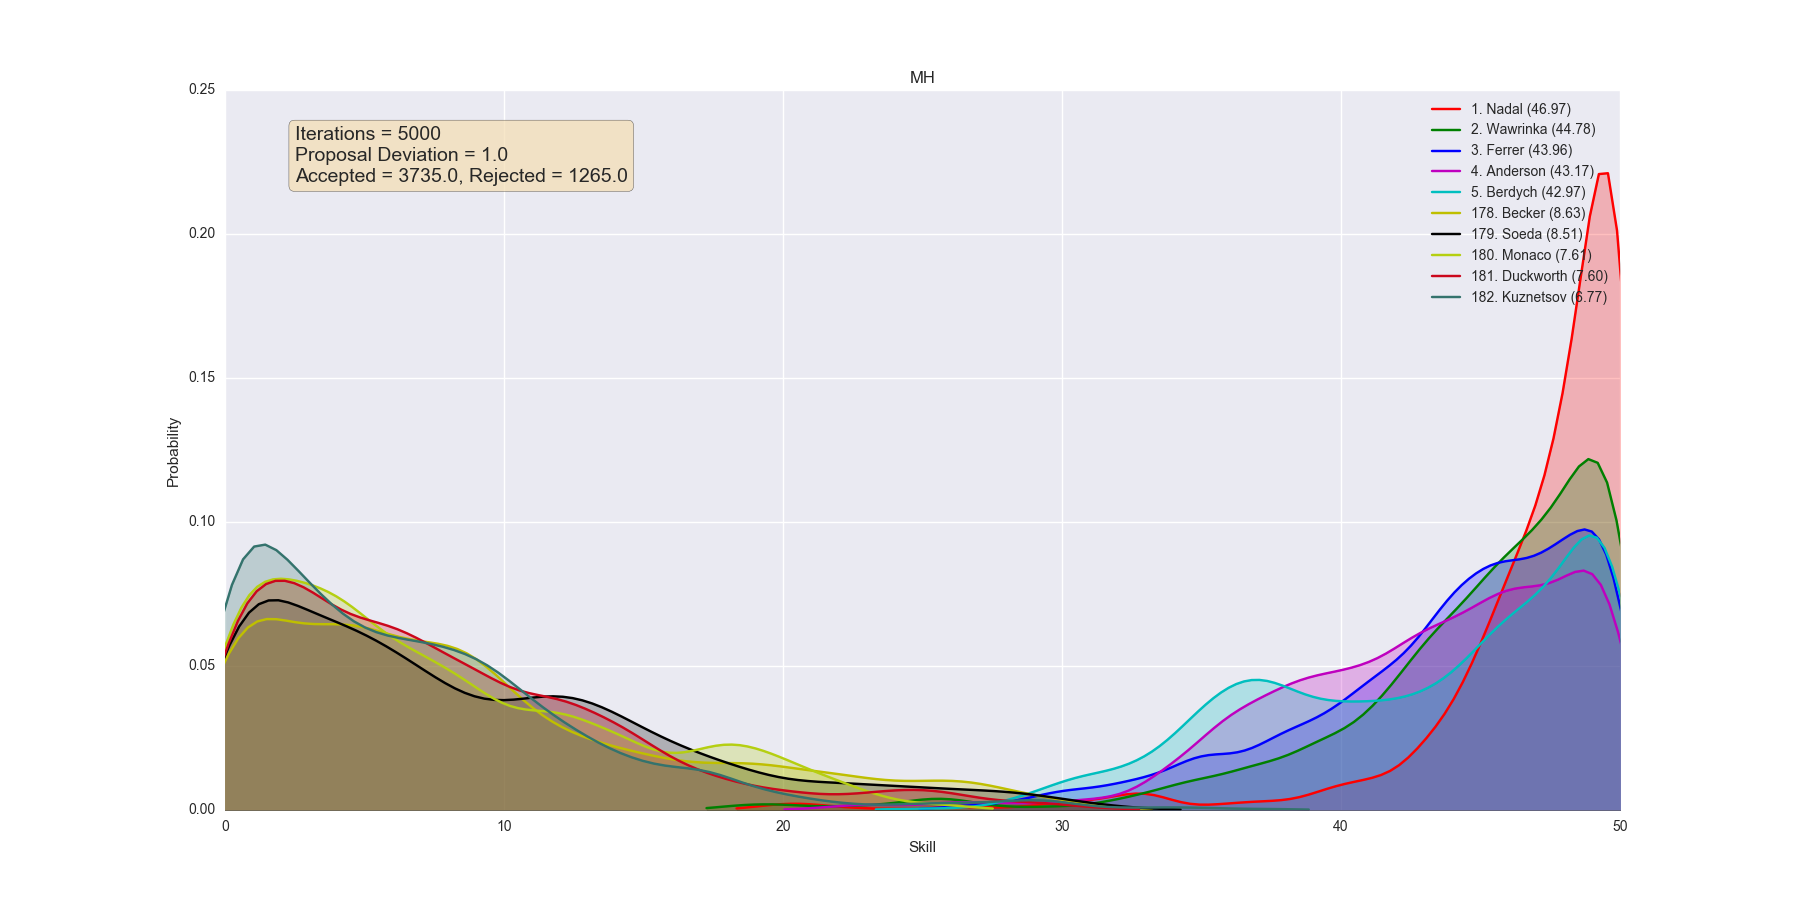
\includegraphics[width=1\columnwidth]{out/T5_13/MH/plot/skill_distribution}
\end{table}
\begin{table}
	\small
	\centering
	\caption{\textbf{Test 5.1}}
	\csvautotabular[respect underscore]{img/out/T5_13/Gibbs/csv/1_signature.csv} \\[5mm]
	\csvautotabular[respect sharp]{img/out/T5_13/Gibbs/csv/3_skills_copy.csv} \hspace{3mm} %
	\csvautotabular[respect sharp]{img/out/T5_13/Gibbs/csv/5_correct_incorrect.csv} \\[5mm]	
	\csvautotabular[respect sharp]{img/out/T5_13/Gibbs/csv/4_predictions_copy.csv} \hspace{3mm}% 
	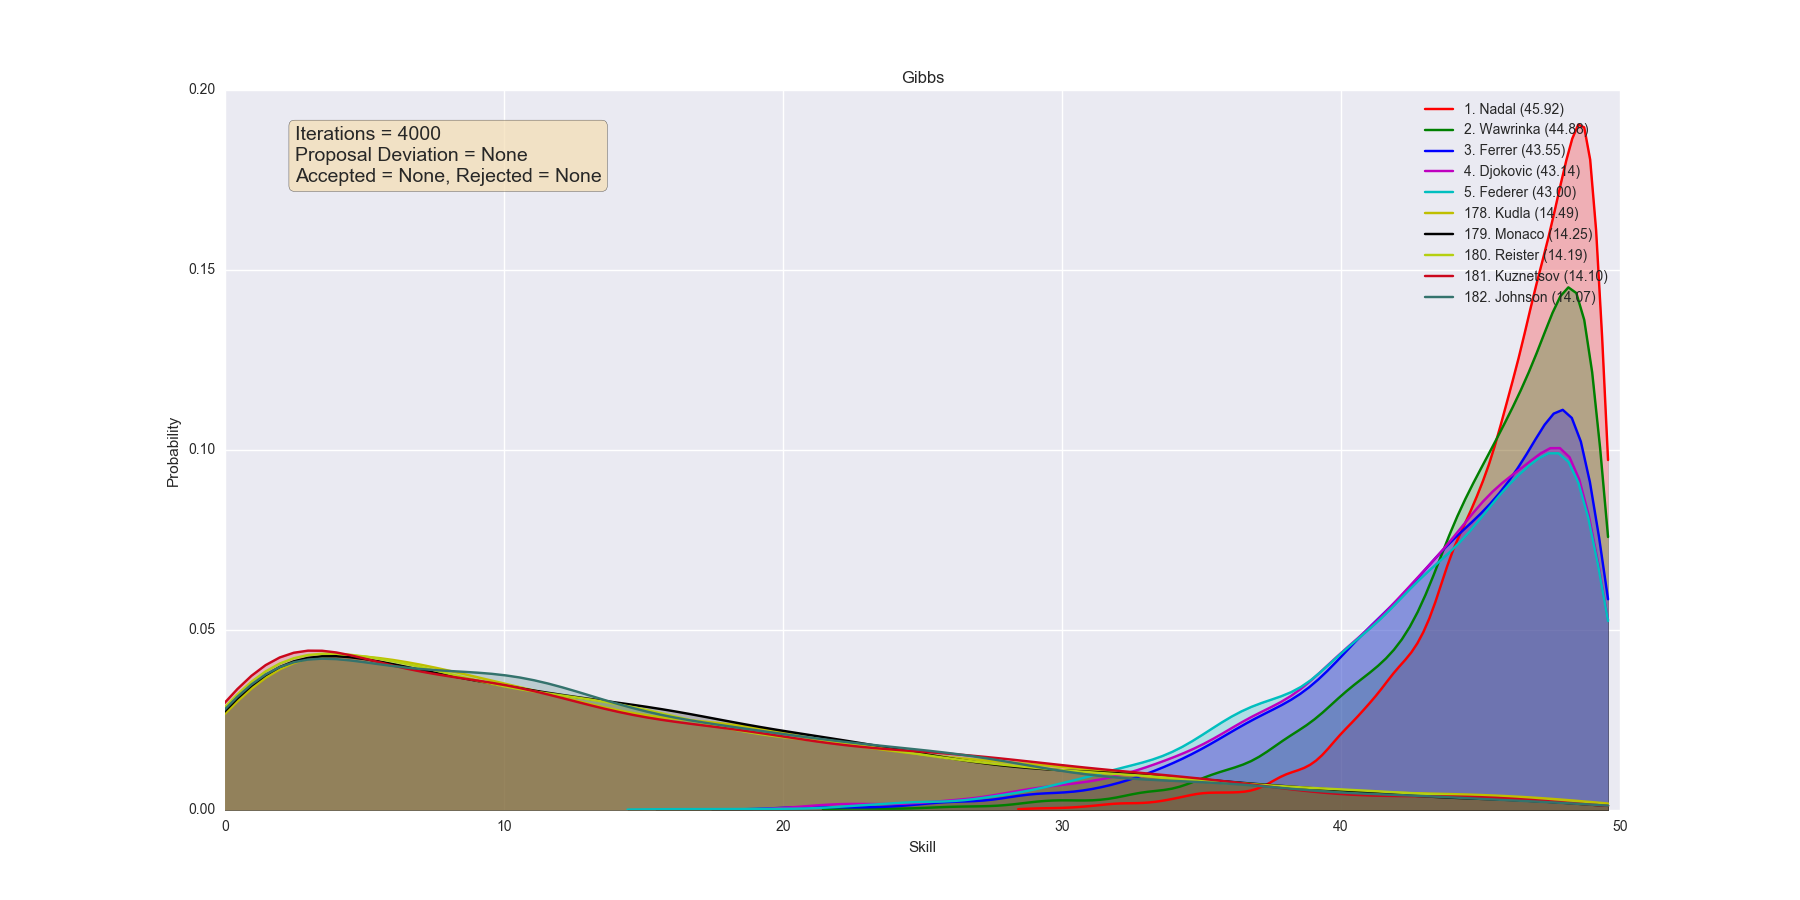
\includegraphics[width=1\columnwidth]{out/T5_13/Gibbs/plot/skill_distribution}
\end{table}
\begin{table}
	\small
	\centering
	\caption{\textbf{Test 5.1}}
	\csvautotabular[respect underscore]{img/out/T5_13/EP/csv/1_signature.csv} \\[5mm]
	\csvautotabular[respect sharp]{img/out/T5_13/EP/csv/3_skills_copy.csv} \hspace{3mm} %
	\csvautotabular[respect sharp]{img/out/T5_13/EP/csv/5_correct_incorrect.csv} \\[5mm]	
	\csvautotabular[respect sharp]{img/out/T5_13/EP/csv/4_predictions_copy.csv} \hspace{3mm}% 
	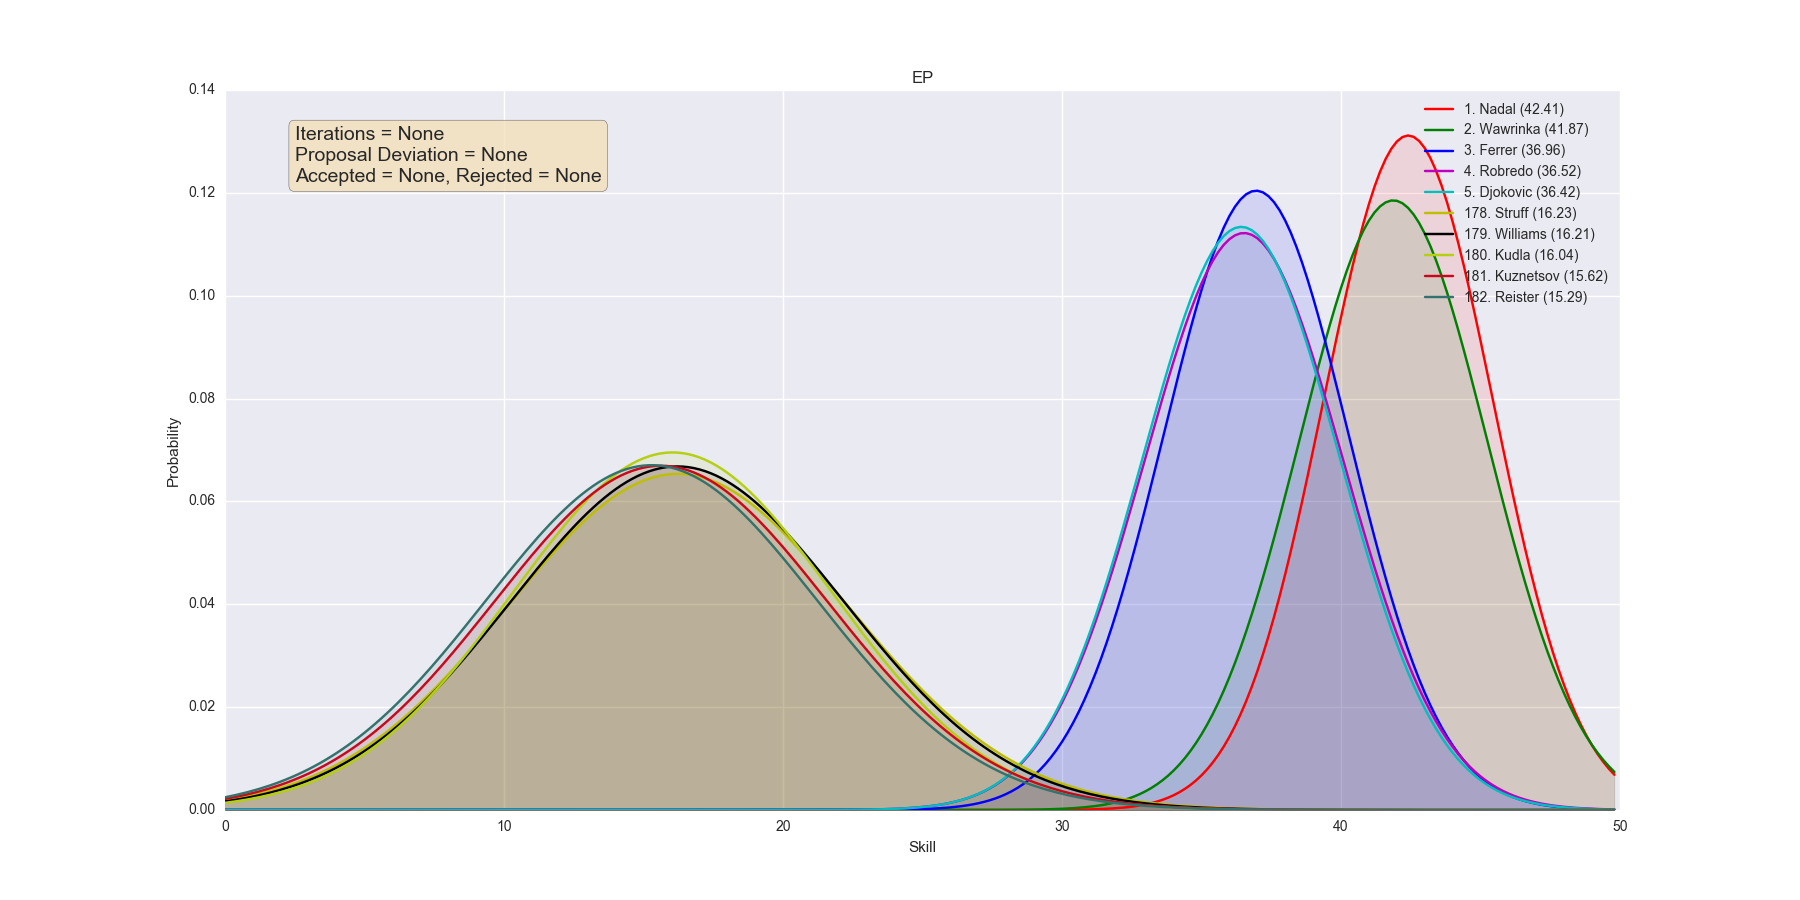
\includegraphics[width=1\columnwidth]{out/T5_13/EP/plot/skill_distribution}
\end{table}




\clearpage
\begin{table}
	\small
	\centering
	\caption{\textbf{Test 5.2}}
	\csvautotabular[respect underscore]{img/out/T5_15/MH/csv/1_signature.csv} \\[5mm]
	\csvautotabular[respect sharp]{img/out/T5_15/MH/csv/3_skills_copy.csv} \hspace{3mm} %
	\raisebox{-.45\height}{\includegraphics[width=0.4\columnwidth]{out/T5_15/MH/plot/actual}}
	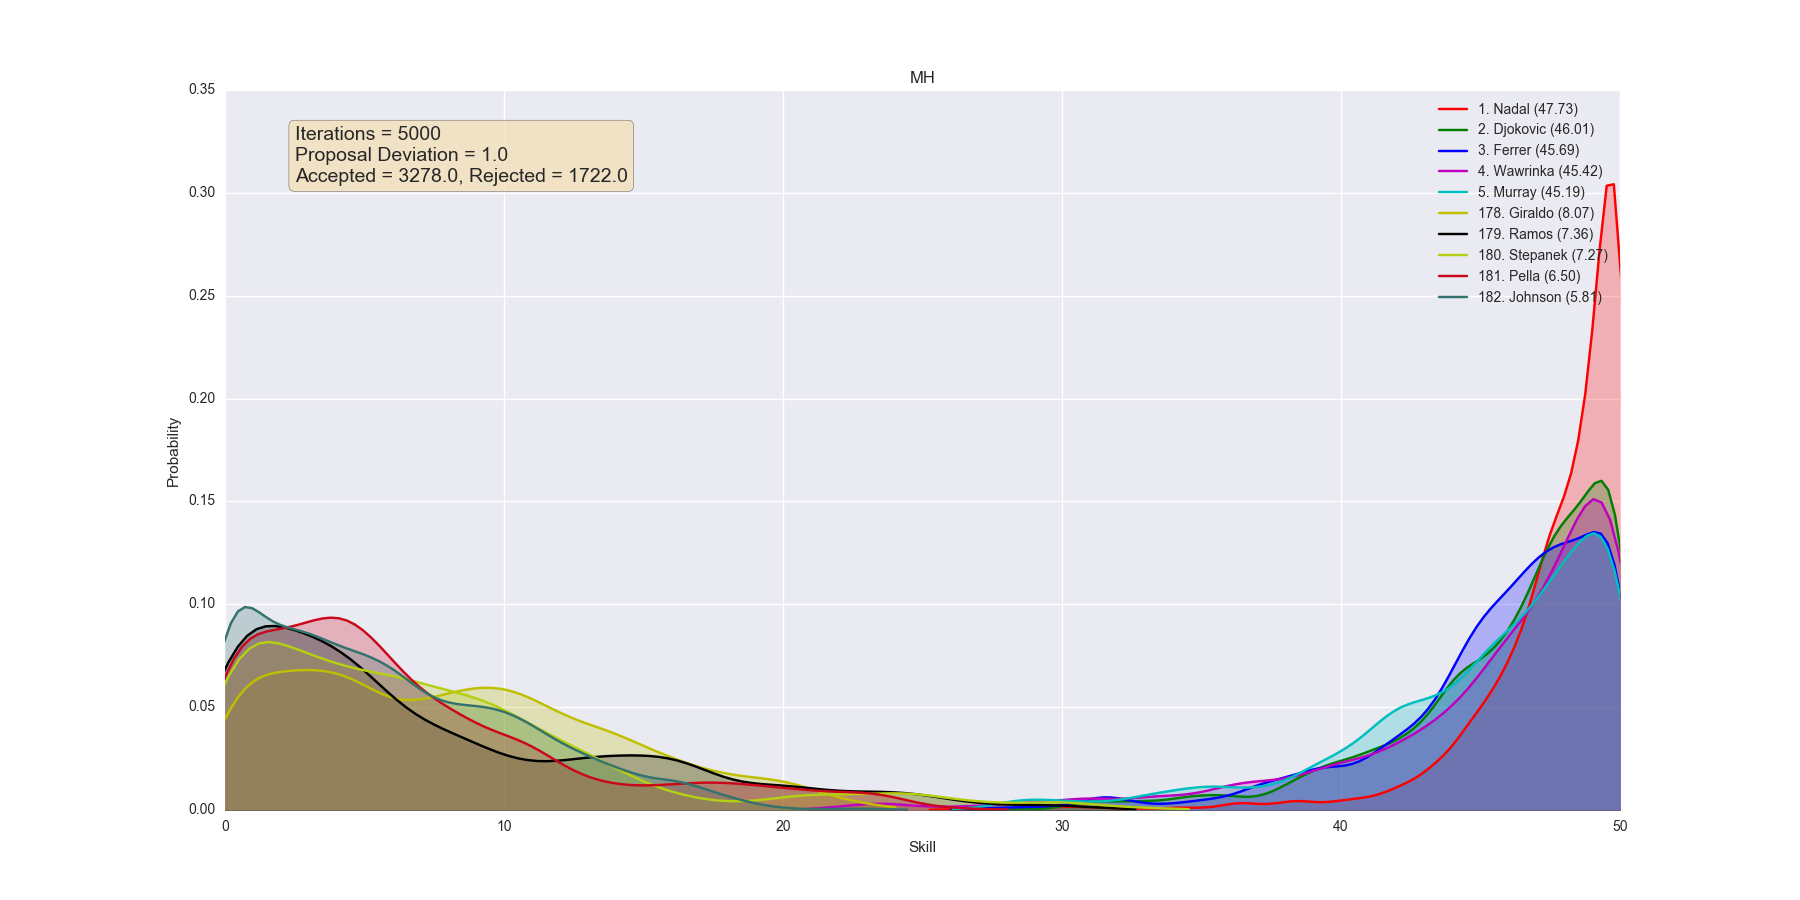
\includegraphics[width=1\columnwidth]{out/T5_15/MH/plot/skill_distribution} %
\end{table}
\begin{table}
	\small
	\centering
	\caption{\textbf{Test 5.2}}
	\csvautotabular[respect underscore]{img/out/T5_15/Gibbs/csv/1_signature.csv} \\[5mm]
	\csvautotabular[respect sharp]{img/out/T5_15/Gibbs/csv/3_skills_copy.csv} \hspace{3mm} %
	\raisebox{-.45\height}{\includegraphics[width=0.4\columnwidth]{out/T5_15/Gibbs/plot/actual}}
	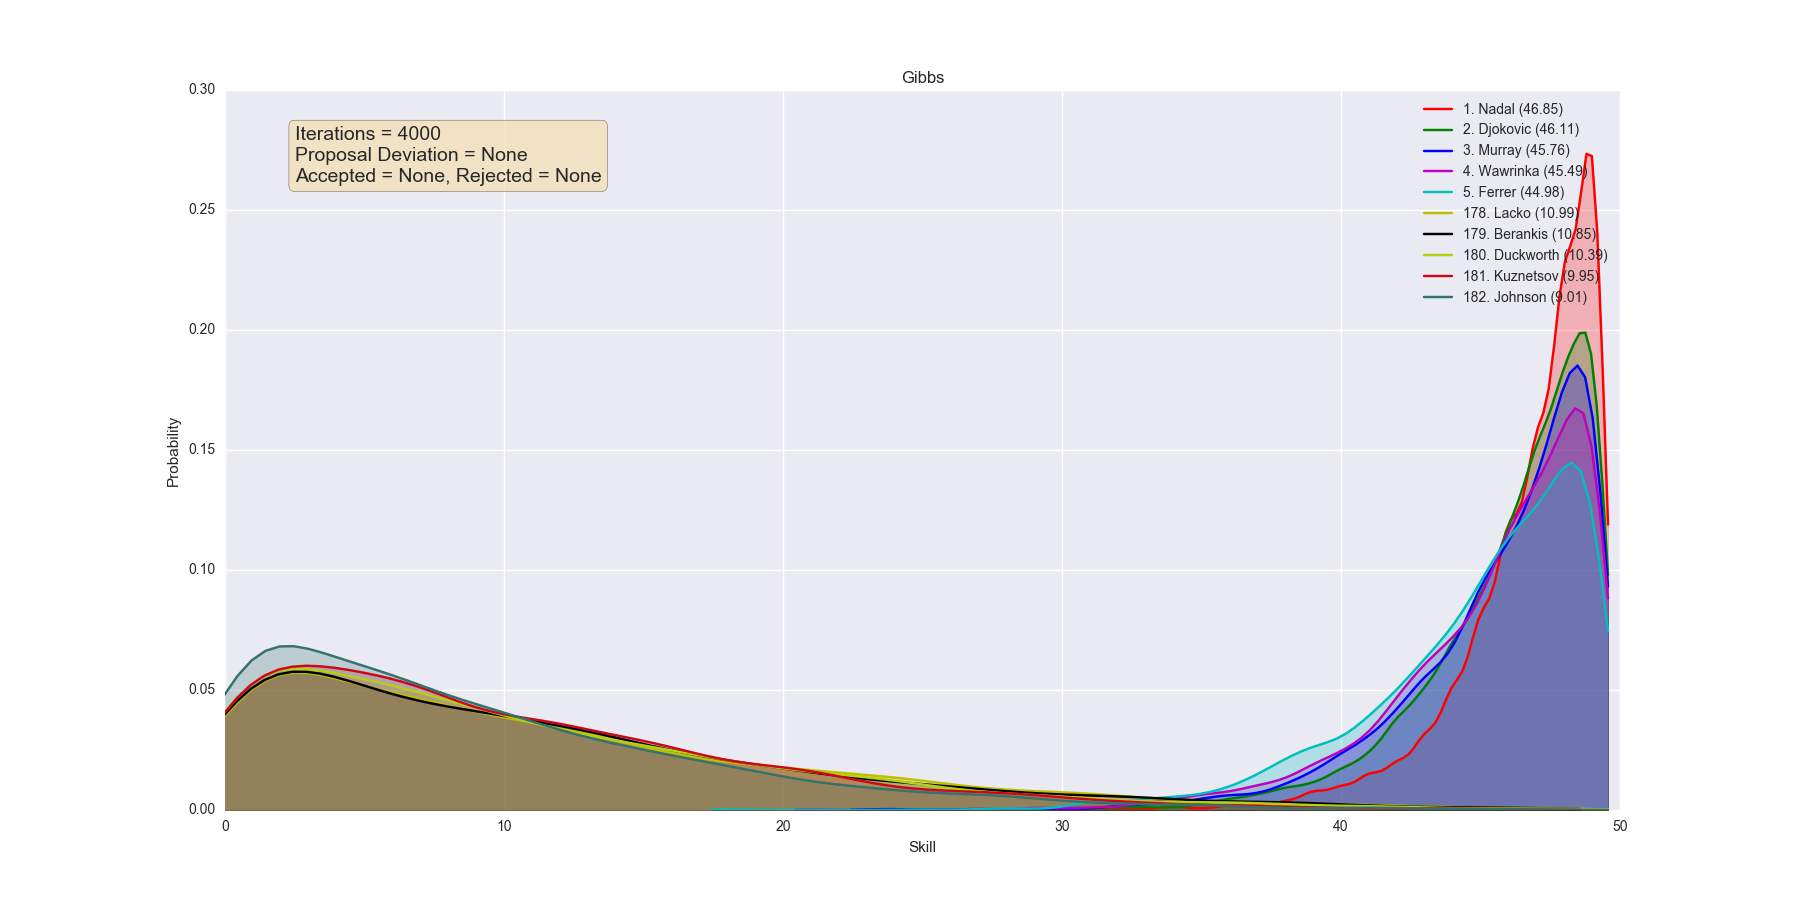
\includegraphics[width=1\columnwidth]{out/T5_15/Gibbs/plot/skill_distribution} %
\end{table}
\begin{table}
	\small
	\centering
	\caption{\textbf{Test 5.2}}
	\csvautotabular[respect underscore]{img/out/T5_15/EP/csv/1_signature.csv} \\[5mm]	
	\csvautotabular[respect sharp]{img/out/T5_15/EP/csv/3_skills_copy.csv} \hspace{5mm} % 
	\raisebox{-.45\height}{\includegraphics[width=0.4\columnwidth]{out/T5_15/EP/plot/actual}}
	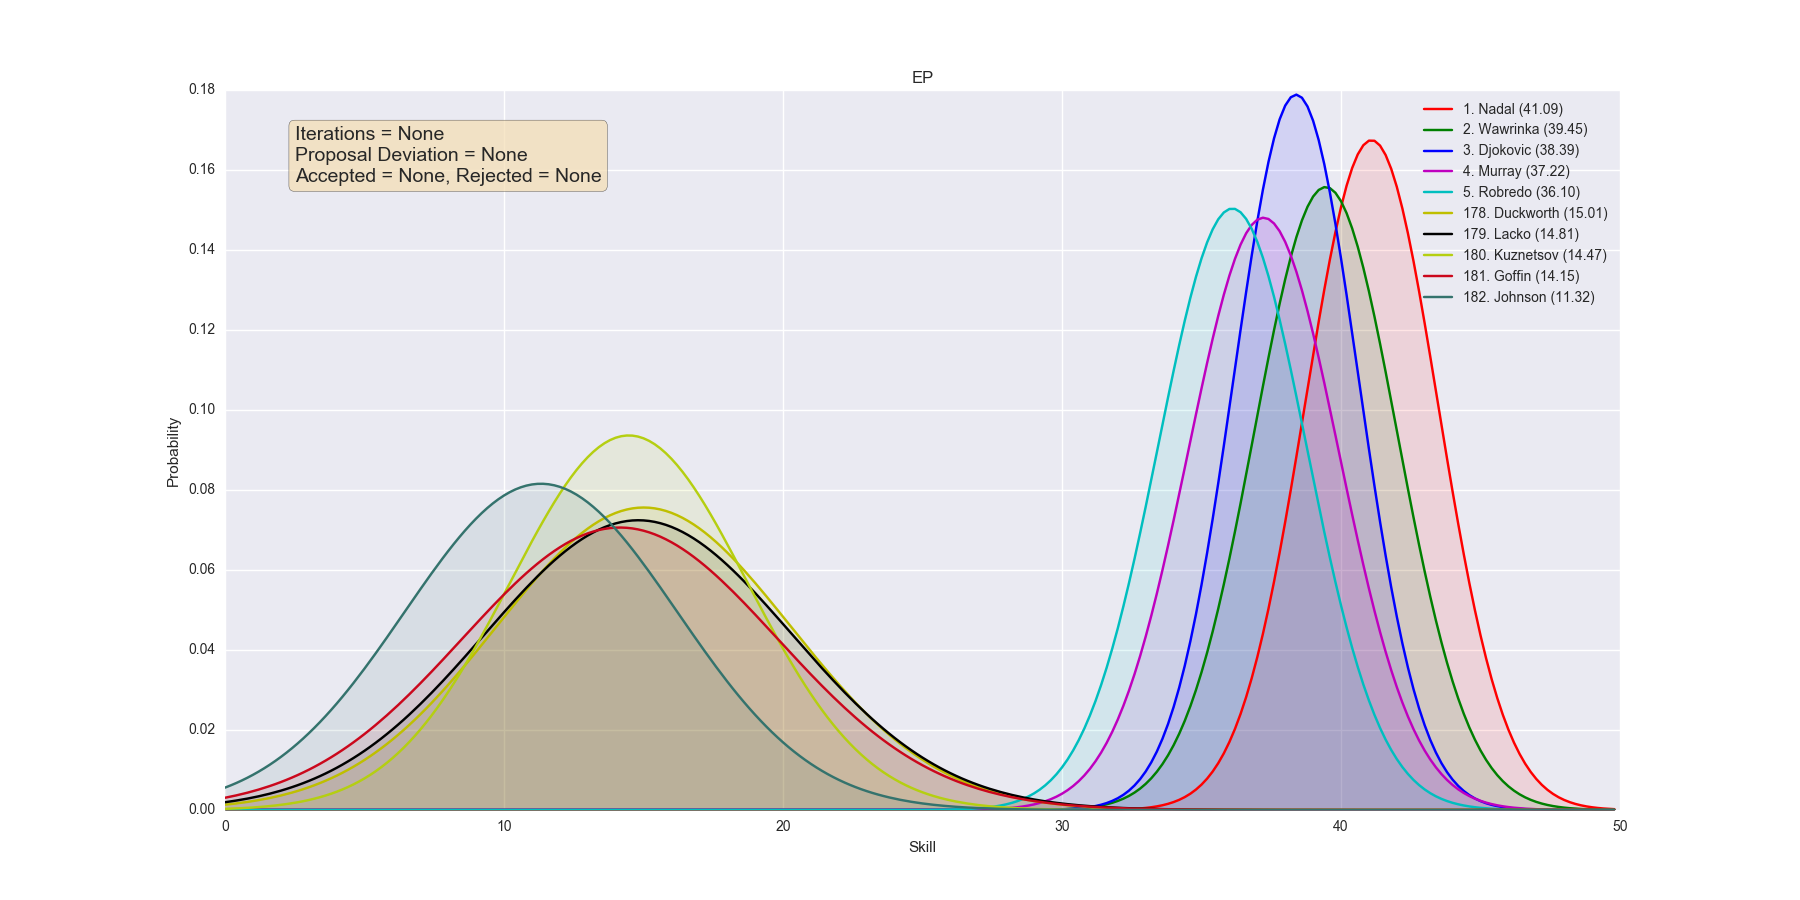
\includegraphics[width=1\columnwidth]{out/T5_15/EP/plot/skill_distribution}
\end{table}




\clearpage
\begin{table}
	\small
	\centering
	\tabcolsep=0.11cm
	\caption{\textbf{Test 6.1}}
	\csvautotabular[respect underscore]{img/out/T6_16/MH/csv/1_signature.csv} \\[5mm]
	\csvautotabular[respect sharp]{img/out/T6_16/MH/csv/3_skills_copy.csv} \hspace{3mm} %
	\csvautotabular[respect sharp]{img/out/T6_16/MH/csv/5_correct_incorrect.csv} \\[5mm]	
	\csvautotabular[respect sharp]{img/out/T6_16/MH/csv/4_predictions_copy.csv} \hspace{3mm}% 
	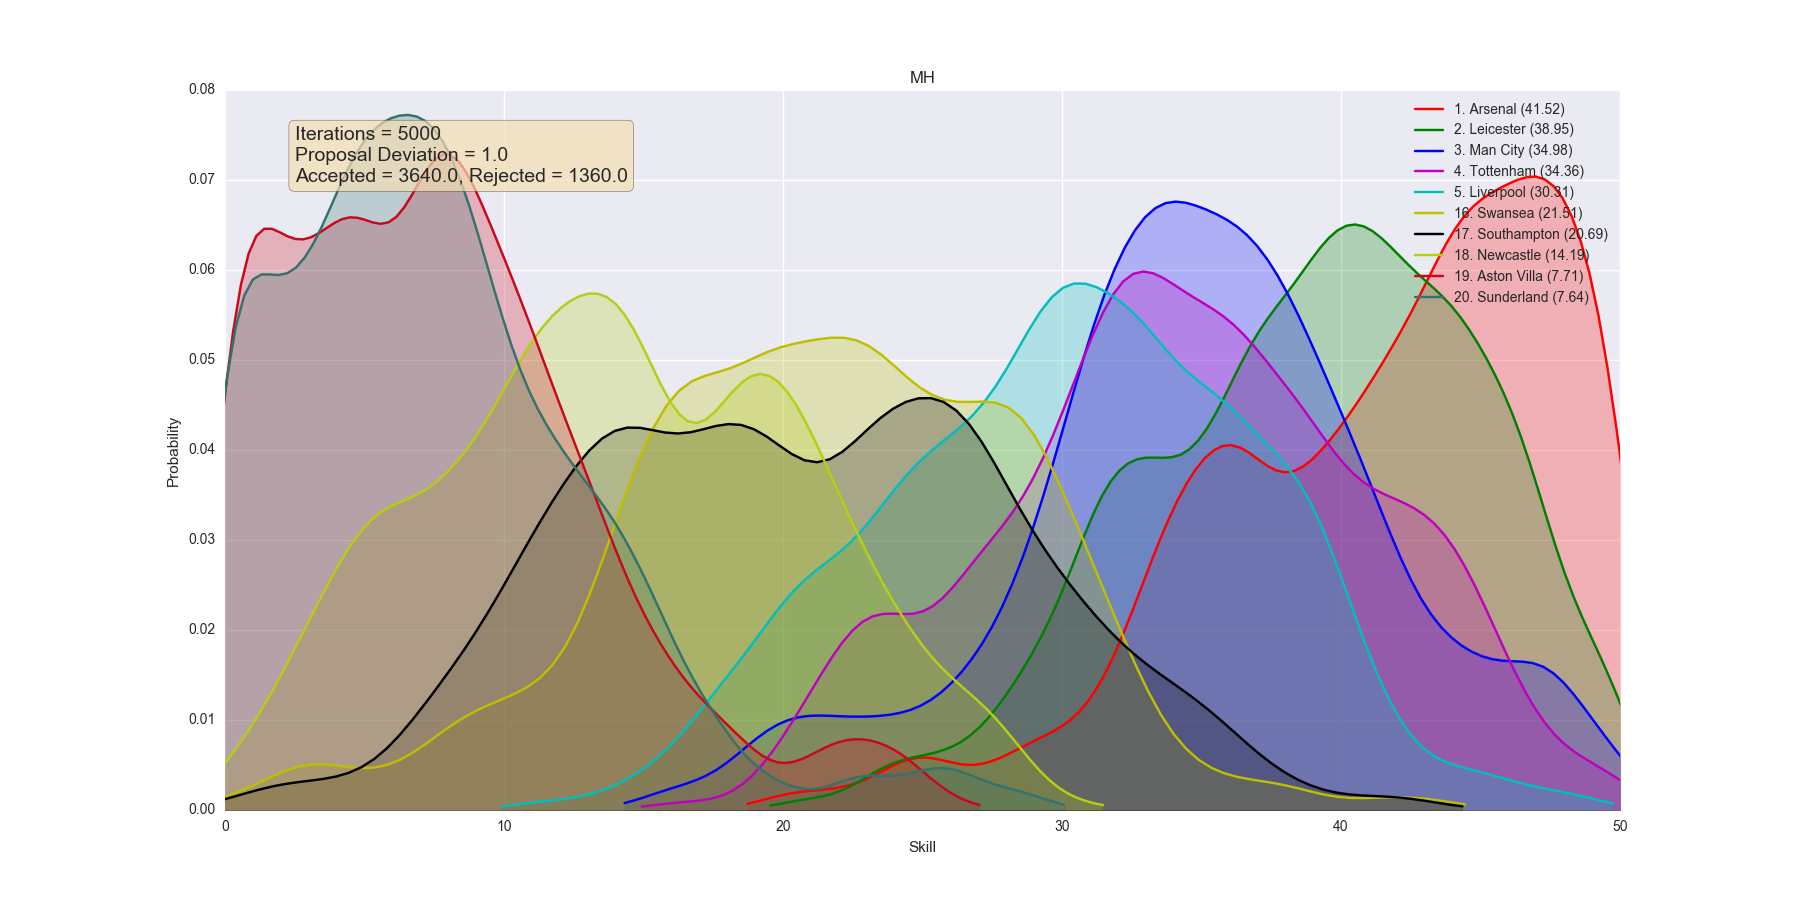
\includegraphics[width=1\columnwidth]{out/T6_16/MH/plot/skill_distribution}
\end{table}
\begin{table}
	\small
	\centering
	\tabcolsep=0.11cm
	\caption{\textbf{Test 6.1}}
	\csvautotabular[respect underscore]{img/out/T6_16/Gibbs/csv/1_signature.csv} \\[5mm]
	\csvautotabular[respect sharp]{img/out/T6_16/Gibbs/csv/3_skills_copy.csv} \hspace{3mm} %
	\csvautotabular[respect sharp]{img/out/T6_16/Gibbs/csv/5_correct_incorrect.csv} \\[5mm]	
	\csvautotabular[respect sharp]{img/out/T6_16/Gibbs/csv/4_predictions_copy.csv} \hspace{3mm}% 
	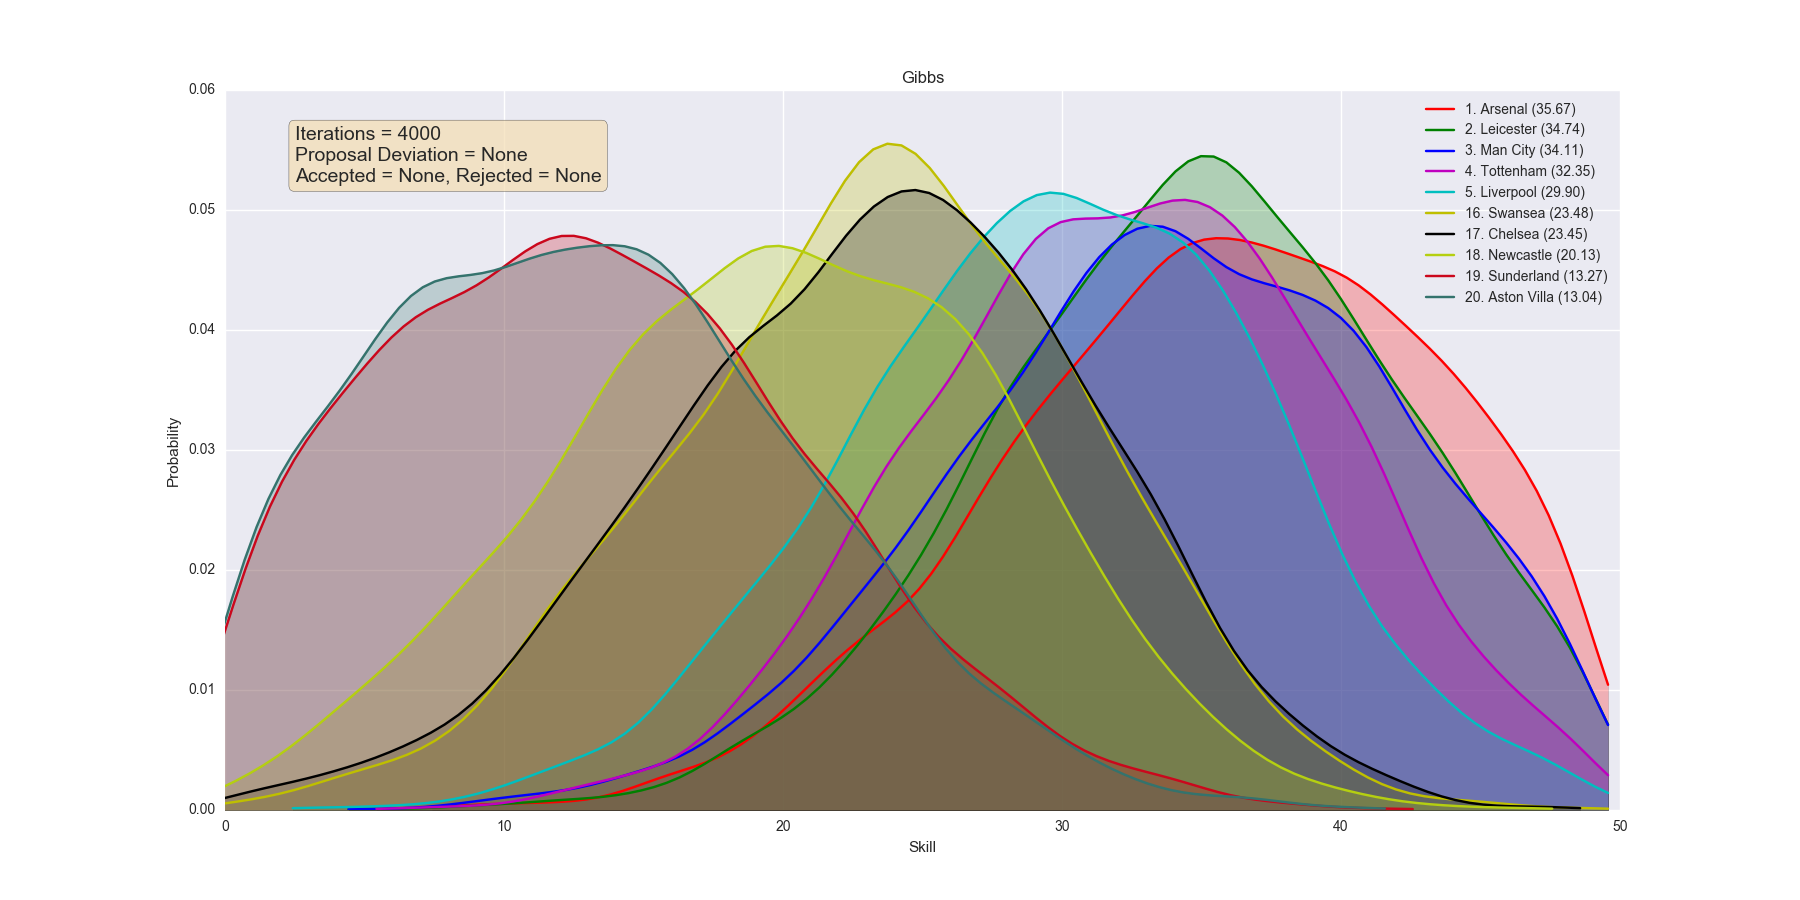
\includegraphics[width=1\columnwidth]{out/T6_16/Gibbs/plot/skill_distribution}
\end{table}
\begin{table}
	\small
	\centering
	\tabcolsep=0.11cm
	\caption{\textbf{Test 6.1}}
	\csvautotabular[respect underscore]{img/out/T6_16/EP/csv/1_signature.csv} \\[5mm]
	\csvautotabular[respect sharp]{img/out/T6_16/EP/csv/3_skills_copy.csv} \hspace{3mm} %
	\csvautotabular[respect sharp]{img/out/T6_16/EP/csv/5_correct_incorrect.csv} \\[5mm]	
	\csvautotabular[respect sharp]{img/out/T6_16/EP/csv/4_predictions_copy.csv} \hspace{3mm}% 
	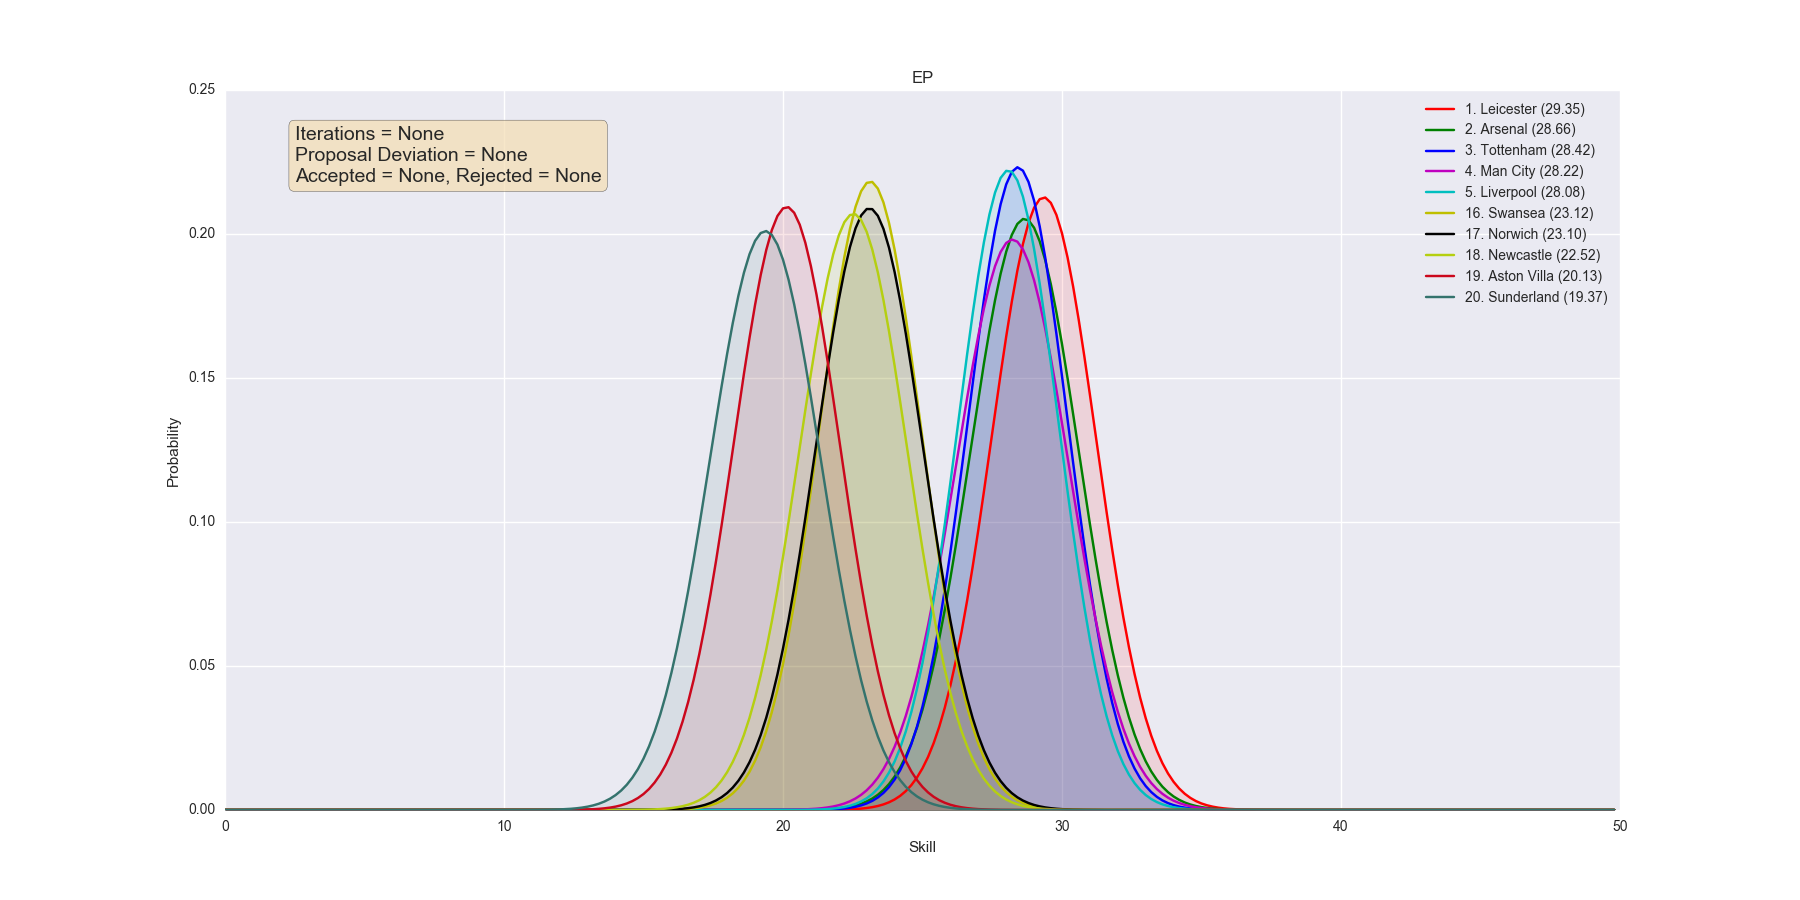
\includegraphics[width=1\columnwidth]{out/T6_16/EP/plot/skill_distribution}
\end{table}




\clearpage
\begin{table}
	\small
	\centering
	\tabcolsep=0.11cm
	\caption{\textbf{Test 6.2}}
	\csvautotabular[respect underscore]{img/out/T6_17/MH/csv/1_signature.csv} \\[5mm]
	\csvautotabular[respect sharp]{img/out/T6_17/MH/csv/3_skills_copy.csv} \hspace{3mm} %
	\csvautotabular[respect sharp]{img/out/T6_17/MH/csv/5_correct_incorrect.csv} \\[5mm]	
	\csvautotabular[respect sharp]{img/out/T6_17/MH/csv/4_predictions_copy.csv} \hspace{3mm}% 
	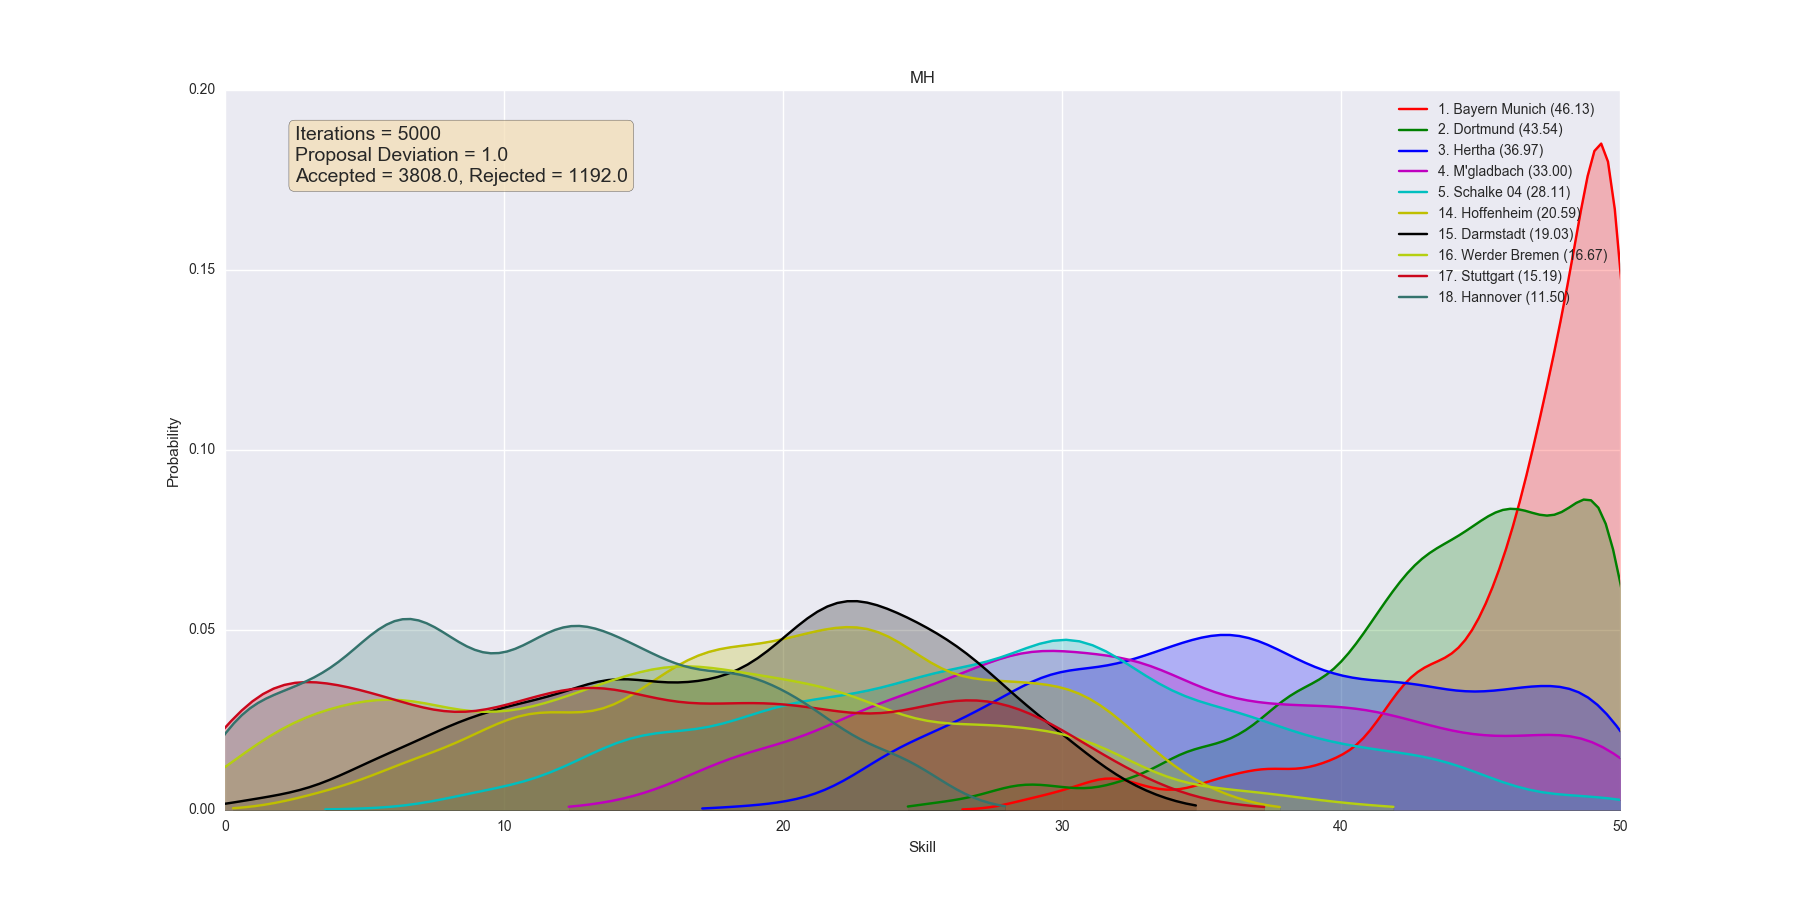
\includegraphics[width=1\columnwidth]{out/T6_17/MH/plot/skill_distribution}
\end{table}
\begin{table}
	\small
	\centering
	\tabcolsep=0.11cm
	\caption{\textbf{Test 6.2}}
	\csvautotabular[respect underscore]{img/out/T6_17/Gibbs/csv/1_signature.csv} \\[5mm]
	\csvautotabular[respect sharp]{img/out/T6_17/Gibbs/csv/3_skills_copy.csv} \hspace{3mm} %
	\csvautotabular[respect sharp]{img/out/T6_17/Gibbs/csv/5_correct_incorrect.csv} \\[5mm]	
	\csvautotabular[respect sharp]{img/out/T6_17/Gibbs/csv/4_predictions_copy.csv} \hspace{3mm}% 
	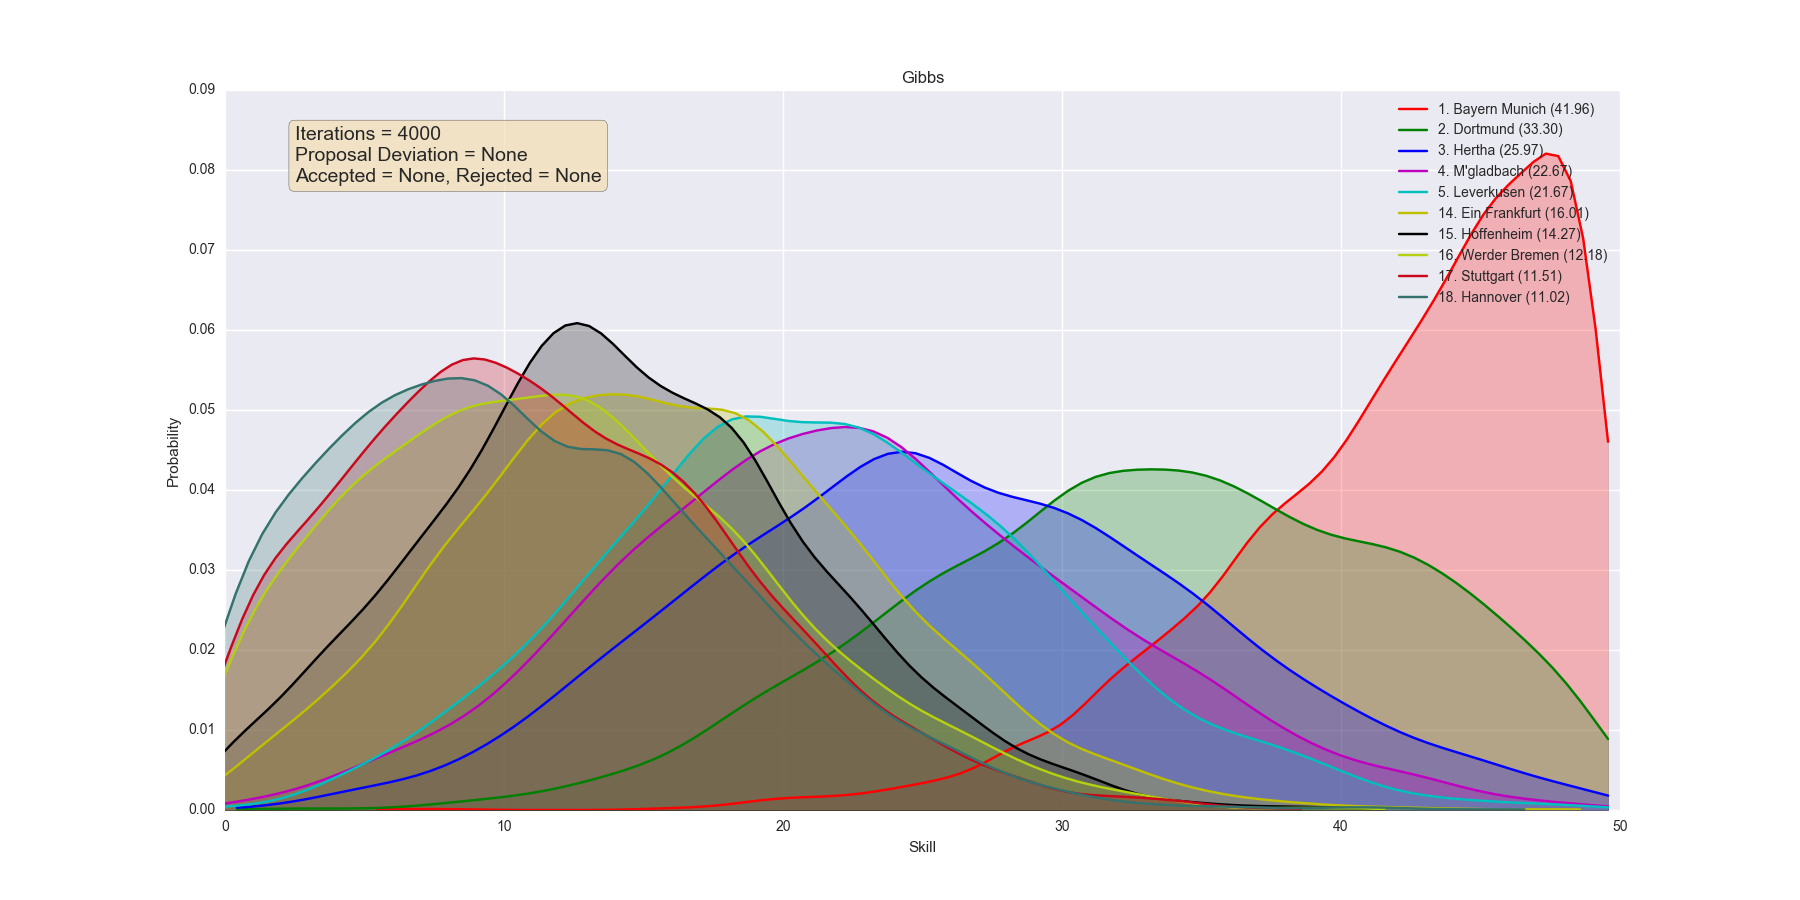
\includegraphics[width=1\columnwidth]{out/T6_17/Gibbs/plot/skill_distribution}
\end{table}
\begin{table}
	\small
	\centering
	\tabcolsep=0.11cm
	\caption{\textbf{Test 6.2}}
	\csvautotabular[respect underscore]{img/out/T6_17/EP/csv/1_signature.csv} \\[5mm]
	\csvautotabular[respect sharp]{img/out/T6_17/EP/csv/3_skills_copy.csv} \hspace{3mm} %
	\csvautotabular[respect sharp]{img/out/T6_17/EP/csv/5_correct_incorrect.csv} \\[5mm]	
	\csvautotabular[respect sharp]{img/out/T6_17/EP/csv/4_predictions_copy.csv} \hspace{3mm}% 
	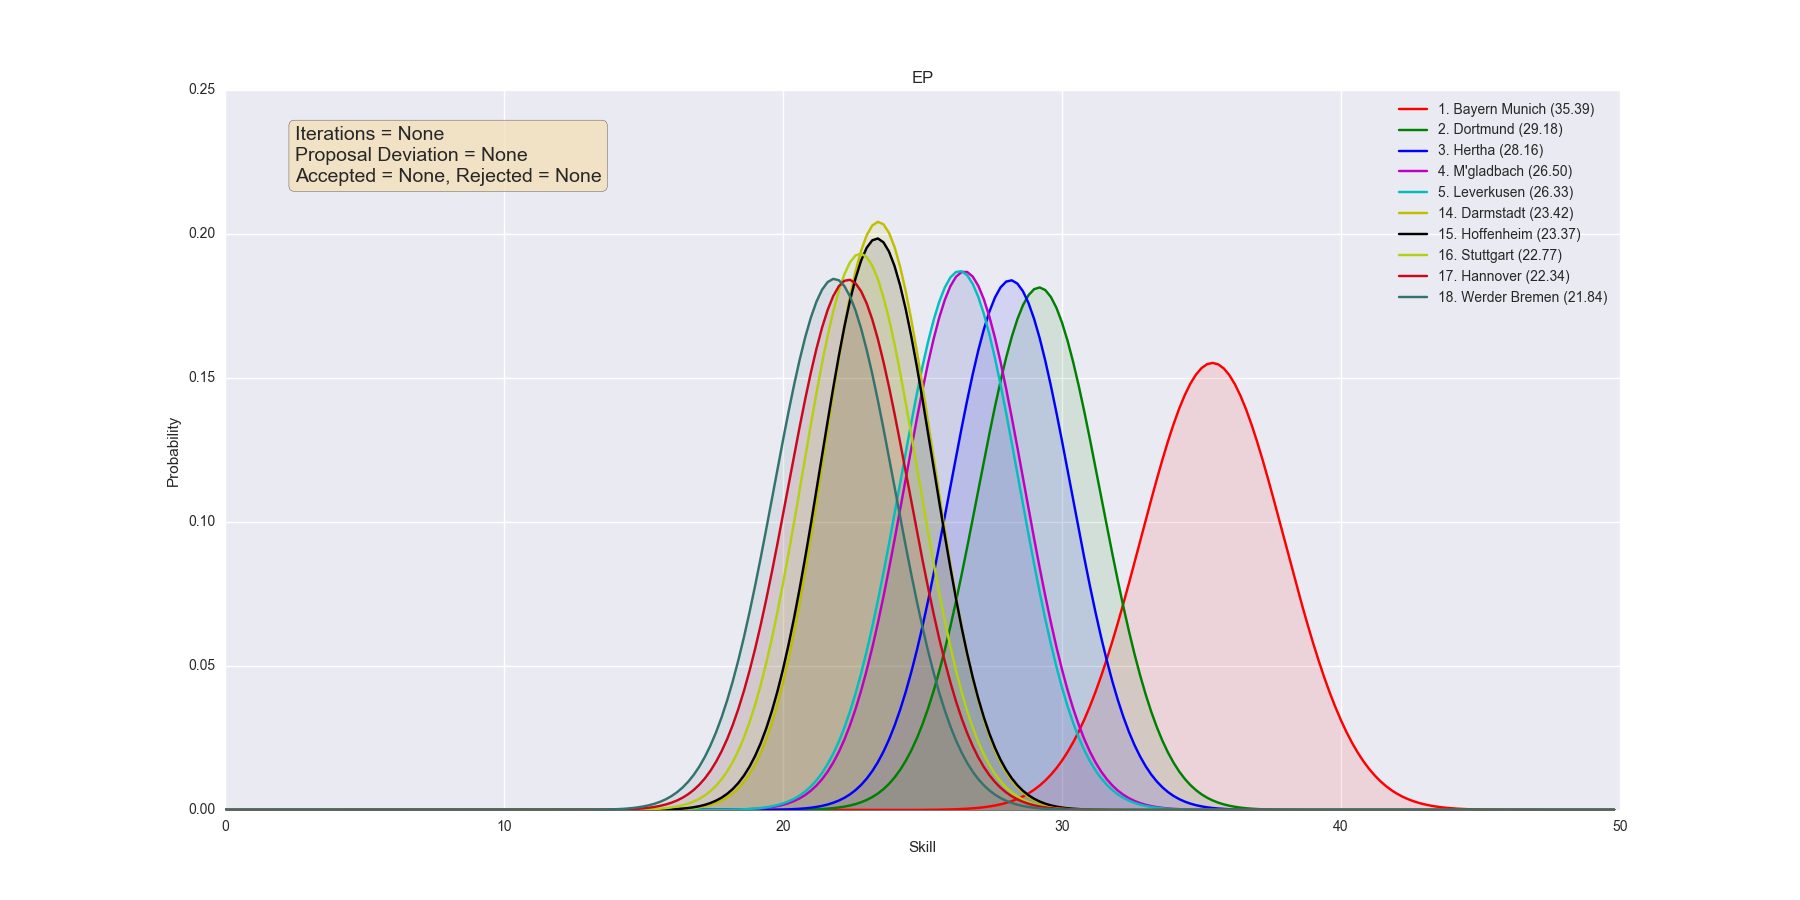
\includegraphics[width=1\columnwidth]{out/T6_17/EP/plot/skill_distribution}
\end{table}




\clearpage
\begin{table}
	\small
	\centering
	\tabcolsep=0.11cm
	\caption{\textbf{Test 6.3}}
	\csvautotabular[respect underscore]{img/out/T6_18/MH/csv/1_signature.csv} \\[5mm]
	\csvautotabular[respect sharp]{img/out/T6_18/MH/csv/3_skills_copy.csv} \hspace{3mm} %
	\csvautotabular[respect sharp]{img/out/T6_18/MH/csv/5_correct_incorrect.csv} \\[5mm]	
	\csvautotabular[respect sharp]{img/out/T6_18/MH/csv/4_predictions_copy.csv} \hspace{3mm}% 
	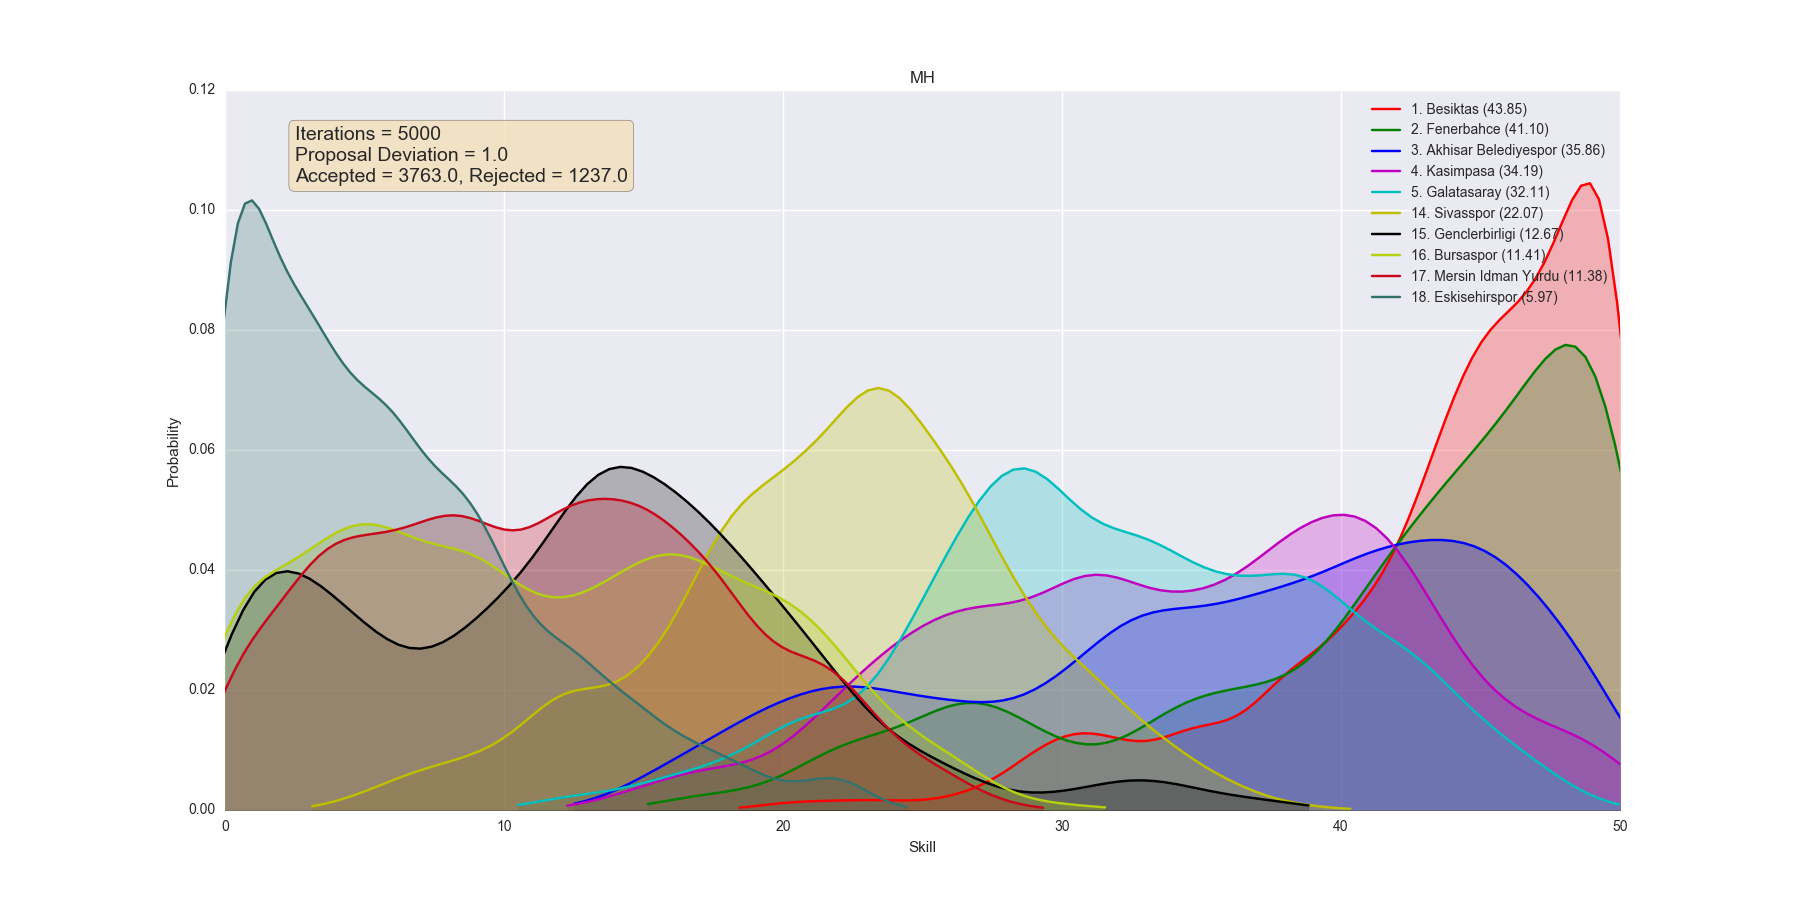
\includegraphics[width=1\columnwidth]{out/T6_18/MH/plot/skill_distribution}
\end{table}
\begin{table}
	\small
	\centering
	\tabcolsep=0.11cm
	\caption{\textbf{Test 6.3}}
	\csvautotabular[respect underscore]{img/out/T6_18/Gibbs/csv/1_signature.csv} \\[5mm]
	\csvautotabular[respect sharp]{img/out/T6_18/Gibbs/csv/3_skills_copy.csv} \hspace{3mm} %
	\csvautotabular[respect sharp]{img/out/T6_18/Gibbs/csv/5_correct_incorrect.csv} \\[5mm]	
	\csvautotabular[respect sharp]{img/out/T6_18/Gibbs/csv/4_predictions_copy.csv} \hspace{3mm}% 
	\includegraphics[width=1\columnwidth]{out/T6_18/Gibbs/plot/skill_distribution}
\end{table}
\begin{table}
	\small
	\centering
	\tabcolsep=0.11cm
	\caption{\textbf{Test 6.3}}
	\csvautotabular[respect underscore]{img/out/T6_18/EP/csv/1_signature.csv} \\[5mm]
	\csvautotabular[respect sharp]{img/out/T6_18/EP/csv/3_skills_copy.csv} \hspace{3mm} %
	\csvautotabular[respect sharp]{img/out/T6_18/EP/csv/5_correct_incorrect.csv} \\[5mm]	
	\csvautotabular[respect sharp]{img/out/T6_18/EP/csv/4_predictions_copy.csv} \hspace{3mm}% 
	\includegraphics[width=1\columnwidth]{out/T6_18/EP/plot/skill_distribution}
\end{table}




\clearpage
\begin{table}
	\small
	\centering
	\tabcolsep=0.11cm
	\caption{\textbf{Test 6.4}}
	\csvautotabular[respect underscore]{img/out/T6_19/MH/csv/1_signature.csv} \\[5mm]
	\csvautotabular[respect sharp]{img/out/T6_19/MH/csv/3_skills_copy.csv} \hspace{3mm} %
	\csvautotabular[respect sharp]{img/out/T6_19/MH/csv/5_correct_incorrect.csv} \\[5mm]	
	\csvautotabular[respect sharp]{img/out/T6_19/MH/csv/4_predictions_copy.csv} \hspace{3mm}% 
	\includegraphics[width=1\columnwidth]{out/T6_19/MH/plot/skill_distribution}
\end{table}
\begin{table}
	\small
	\centering
	\tabcolsep=0.11cm
	\caption{\textbf{Test 6.4}}
	\csvautotabular[respect underscore]{img/out/T6_19/Gibbs/csv/1_signature.csv} \\[5mm]
	\csvautotabular[respect sharp]{img/out/T6_19/Gibbs/csv/3_skills_copy.csv} \hspace{3mm} %
	\csvautotabular[respect sharp]{img/out/T6_19/Gibbs/csv/5_correct_incorrect.csv} \\[5mm]	
	\csvautotabular[respect sharp]{img/out/T6_19/Gibbs/csv/4_predictions_copy.csv} \hspace{3mm}% 
	\includegraphics[width=1\columnwidth]{out/T6_19/Gibbs/plot/skill_distribution}
\end{table}
\begin{table}
	\small
	\centering
	\tabcolsep=0.11cm
	\caption{\textbf{Test 6.4}}
	\csvautotabular[respect underscore]{img/out/T6_19/EP/csv/1_signature.csv} \\[5mm]
	\csvautotabular[respect sharp]{img/out/T6_19/EP/csv/3_skills_copy.csv} \hspace{3mm} %
	\csvautotabular[respect sharp]{img/out/T6_19/EP/csv/5_correct_incorrect.csv} \\[5mm]	
	\csvautotabular[respect sharp]{img/out/T6_19/EP/csv/4_predictions_copy.csv} \hspace{3mm}% 
	\includegraphics[width=1\columnwidth]{out/T6_19/EP/plot/skill_distribution}
\end{table}



\clearpage
\begin{table}
	\small
	\centering
	\caption{\textbf{Test 6.5}}
	\csvautotabular[respect underscore]{img/out/T6_20/MH/csv/1_signature.csv} \\[5mm]
	\csvautotabular[respect sharp]{img/out/T6_20/MH/csv/3_skills_copy.csv} \hspace{3mm} %
	\raisebox{-.45\height}{\includegraphics[width=0.4\columnwidth]{out/T6_20/MH/plot/actual}}
	\includegraphics[width=1\columnwidth]{out/T6_20/MH/plot/skill_distribution} %
\end{table}
\begin{table}
	\small
	\centering
	\caption{\textbf{Test 6.5}}
	\csvautotabular[respect underscore]{img/out/T6_20/Gibbs/csv/1_signature.csv} \\[5mm]
	\csvautotabular[respect sharp]{img/out/T6_20/Gibbs/csv/3_skills_copy.csv} \hspace{3mm} %
	\raisebox{-.45\height}{\includegraphics[width=0.4\columnwidth]{out/T6_20/Gibbs/plot/actual}}
	\includegraphics[width=1\columnwidth]{out/T6_20/Gibbs/plot/skill_distribution} %
\end{table}
\begin{table}
	\small
	\centering
	\caption{\textbf{Test 6.5}}
	\csvautotabular[respect underscore]{img/out/T6_20/EP/csv/1_signature.csv} \\[5mm]	
	\csvautotabular[respect sharp]{img/out/T6_20/EP/csv/3_skills_copy.csv} \hspace{3mm} % 
	\raisebox{-.45\height}{\includegraphics[width=0.4\columnwidth]{out/T6_20/EP/plot/actual}}
	\includegraphics[width=1\columnwidth]{out/T6_20/EP/plot/skill_distribution}
\end{table}




\clearpage
\begin{table}
	\small
	\centering
	\tabcolsep=0.11cm
	\caption{\textbf{Test 7.1}}
	\csvautotabular[respect underscore]{img/out/T7_21/MH/csv/1_signature.csv} \\[5mm]
	\csvautotabular[respect sharp]{img/out/T7_21/MH/csv/3_skills_copy.csv} \hspace{3mm} %
	\csvautotabular[respect sharp]{img/out/T7_21/MH/csv/5_correct_incorrect.csv} \\[5mm]	
	\csvautotabular[respect sharp]{img/out/T7_21/MH/csv/4_predictions_copy.csv} \hspace{3mm}% 
	\includegraphics[width=1\columnwidth]{out/T7_21/MH/plot/skill_distribution}
\end{table}
\begin{table}
	\small
	\centering
	\tabcolsep=0.11cm
	\caption{\textbf{Test 7.1}}
	\csvautotabular[respect underscore]{img/out/T7_21/Gibbs/csv/1_signature.csv} \\[5mm]
	\csvautotabular[respect sharp]{img/out/T7_21/Gibbs/csv/3_skills_copy.csv} \hspace{3mm} %
	\csvautotabular[respect sharp]{img/out/T7_21/Gibbs/csv/5_correct_incorrect.csv} \\[5mm]	
	\csvautotabular[respect sharp]{img/out/T7_21/Gibbs/csv/4_predictions_copy.csv} \hspace{3mm}% 
	\includegraphics[width=1\columnwidth]{out/T7_21/Gibbs/plot/skill_distribution}
\end{table}
\begin{table}
	\small
	\centering
	\tabcolsep=0.11cm
	\caption{\textbf{Test 7.1}}
	\csvautotabular[respect underscore]{img/out/T7_21/EP/csv/1_signature.csv} \\[5mm]
	\csvautotabular[respect sharp]{img/out/T7_21/EP/csv/3_skills_copy.csv} \hspace{3mm} %
	\csvautotabular[respect sharp]{img/out/T7_21/EP/csv/5_correct_incorrect.csv} \\[5mm]	
	\csvautotabular[respect sharp]{img/out/T7_21/EP/csv/4_predictions_copy.csv} \hspace{3mm}% 
	\includegraphics[width=1\columnwidth]{out/T7_21/EP/plot/skill_distribution}
\end{table}



\clearpage
\begin{table}
	\small
	\centering
	\caption{\textbf{Test 7.2}}
	\csvautotabular[respect underscore]{img/out/T7_22/MH/csv/1_signature.csv} \\[5mm]
	\csvautotabular[respect sharp]{img/out/T7_22/MH/csv/3_skills_copy.csv} \hspace{1mm} %
	\raisebox{-.45\height}{\includegraphics[width=0.22\columnwidth]{out/T7_22/MH/plot/actual1}} %
	\raisebox{-.45\height}{\includegraphics[width=0.22\columnwidth]{out/T7_22/MH/plot/actual2}}
	\includegraphics[width=1\columnwidth]{out/T7_22/MH/plot/skill_distribution} %
\end{table}
\begin{table}
	\small
	\centering
	\caption{\textbf{Test 7.2}}
	\csvautotabular[respect underscore]{img/out/T7_22/Gibbs/csv/1_signature.csv} \\[5mm]
	\csvautotabular[respect sharp]{img/out/T7_22/Gibbs/csv/3_skills_copy.csv} \hspace{3mm} %
	\raisebox{-.45\height}{\includegraphics[width=0.22\columnwidth]{out/T7_22/Gibbs/plot/actual1}} %
	\raisebox{-.45\height}{\includegraphics[width=0.22\columnwidth]{out/T7_22/Gibbs/plot/actual2}}
	\includegraphics[width=1\columnwidth]{out/T7_22/Gibbs/plot/skill_distribution} %
\end{table}
\begin{table}
	\small
	\centering
	\caption{\textbf{Test 7.2}}
	\csvautotabular[respect underscore]{img/out/T7_22/EP/csv/1_signature.csv} \\[5mm]	
	\csvautotabular[respect sharp]{img/out/T7_22/EP/csv/3_skills_copy.csv} \hspace{3mm} % 
	\raisebox{-.45\height}{\includegraphics[width=0.22\columnwidth]{out/T7_22/EP/plot/actual1}} %
	\raisebox{-.45\height}{\includegraphics[width=0.22\columnwidth]{out/T7_22/EP/plot/actual2}}
	\includegraphics[width=1\columnwidth]{out/T7_22/EP/plot/skill_distribution}
\end{table}
\clearpage









%\newpage
%\section{Appendices}
%\lstinputlisting[breaklines=true, language=Python,basicstyle=\footnotesize,numbers=left,frame=single]{../source/main.py}

%\lstinputlisting[breaklines=true, language=Python,basicstyle=\footnotesize,numbers=left,frame=single]{../source/test.py}

%\lstinputlisting[breaklines=true, language=Python,basicstyle=\footnotesize,numbers=left,frame=single]{../source/reader.py}

%\lstinputlisting[breaklines=true, language=Python,basicstyle=\footnotesize,numbers=left,frame=single]{../source/model.py}

%\lstinputlisting[breaklines=true, language=Python,basicstyle=\footnotesize,numbers=left,frame=single]{../source/mc.py}

%\lstinputlisting[breaklines=true, language=Python,basicstyle=\footnotesize,numbers=left,frame=single]{../source/ep.py}

%\lstinputlisting[breaklines=true, language=Python,basicstyle=\footnotesize,numbers=left,frame=single]{../source/evaluate.py}

%\lstinputlisting[breaklines=true, language=Python,basicstyle=\footnotesize,numbers=left,frame=single]{../source/factory.py}


\end{document}
